\chapter{Results and Discussion}\label{chap:results}

\section*{}

This chapter intends to present the results for both the several performed machine learning runs using different algorithms and different features as well as different combinations of features and the naive implementations. By analysing the results using visual cues and the evaluation metrics previously defined in chapter \ref{chap:method}, the upcoming findings suggest if the machine learning techniques are correctly predicting the breast deformation. The results will also be further analysed in order to understand on which regions of the breast, the prediction is more inaccurate in terms of distance between the predicted and the real data. 

The current chapter is divided into 3 sections, being the first two, section \ref{sec:naive_results} and section \ref{sec:ml_results}, used to shown the visual and evaluation metrics' results for the naive methods and the machine learning models respectively. Section \ref{sec:heatmap} will present the regions of the breast where the predictions are more inaccurate.
All the results and intermediary conclusions will be used to draw the final conclusions present in chapter \ref{chap:concl}.

\section{Naive Method Results} \label{sec:naive_results}

As described before, two different naive methods approaches were tried in order to predicted the deformation caused by BCS. The implementation of this approach has as goal, understanding the improvement provided by the use of machine learning techniques instead of using methods based on common sense and the findings resultant from the feature analysis in section \ref{subsec:feat_analysis}.

Table \ref{tab:naive1} shows the global evaluation metrics for the the naive method described in section \ref{sub_sec:naive_method_explanation} that uses the geometric center of the breast in order to divide it into quadrants. Table \ref{tab:naive1_local} represents the local evaluation metrics in the same conditions. As shown the prediction made by the naive method leads to the movement, not very significant, of the breast's. This effect can be visualized in Figure \ref{fig:naive1}. Using this method leads to an over prediction of the displacement in cases similar to the one represented in Figure \ref{fig:naive1_left}, where the the breast suffers a minor deformation caused by the BCS and to an under prediction of the displacement in cases similar to the one represented in Figure \ref{fig:naive1_right}, where the breast's deformation caused by the BCS is more severe. 

% Please add the following required packages to your document preamble:
% \usepackage{multirow}
\begin{table}[!htb]
\centering
\begin{tabular}{lll|l|l|l|l|l|l|}
\cline{4-9}
                                                   &                                                                                                             &                                                                       & \textbf{\begin{tabular}[c]{@{}l@{}}predicted\\  to pos\end{tabular}} & \textbf{\begin{tabular}[c]{@{}l@{}}pos to \\ predicted\end{tabular}} & \textbf{pre to pos} & \textbf{pos to pre} & \textbf{\begin{tabular}[c]{@{}l@{}}predicted\\  to pre\end{tabular}} & \textbf{\begin{tabular}[c]{@{}l@{}}pre to \\ predicted\end{tabular}} \\ \hline
\multicolumn{1}{|l|}{\multirow{3}{*}{\textbf{3D}}} & \multicolumn{1}{l|}{\multirow{2}{*}{\textbf{\begin{tabular}[c]{@{}l@{}}Euclidean\\ Distance\end{tabular}}}} & \textbf{Mean}                                                         & 1.731                                                                & 1.725                                                                & 1.758               & 1.731               & 1.420                                                                & 1.421                                                                \\ \cline{3-9} 
\multicolumn{1}{|l|}{}                             & \multicolumn{1}{l|}{}                                                                                       & \textbf{\begin{tabular}[c]{@{}l@{}}Standard\\ Deviation\end{tabular}} & 1.130                                                                & 1.113                                                                & 1.333               & 1.277               & 1.064                                                                & 1.394                                                                \\ \cline{2-9} 
\multicolumn{1}{|l|}{}                             & \multicolumn{2}{l|}{\textbf{\begin{tabular}[c]{@{}l@{}}Hausdorff Distance\end{tabular}}}                                                                                          & 5.563                                                                & 5.539                                                                & 6.513               & 6.317               & 2.939                                                                & 6.452                                                                \\ \hline
\multicolumn{1}{|l|}{\multirow{3}{*}{\textbf{1D}}} & \multicolumn{1}{l|}{\multirow{2}{*}{\textbf{\begin{tabular}[c]{@{}l@{}}Euclidean\\ Distance\end{tabular}}}} & \textbf{Mean}                                                         & 0.141                                                                & 0.123                                                                & 0.160               & 0.110               & 0.113                                                                & 0.083                                                                \\ \cline{3-9} 
\multicolumn{1}{|l|}{}                             & \multicolumn{1}{l|}{}                                                                                       & \textbf{\begin{tabular}[c]{@{}l@{}}Standard\\ Deviation\end{tabular}} & 0.210                                                                & 0.145                                                                & 0.346               & 0.110               & 0.142                                                                & 0.243                                                                \\ \cline{2-9} 
\multicolumn{1}{|l|}{}                             & \multicolumn{2}{l|}{\textbf{\begin{tabular}[c]{@{}l@{}}Hausdorff Distance\end{tabular}}}                                                                                          & 1.631                                                                & 1.203                                                                & 3.168               & 0.704               & 0.787                                                                & 3.325                                                                \\ \hline
\end{tabular}
\caption{Global Evaluation Metrics for the first approach of the naive method}
\label{tab:naive1}
\end{table}

\begin{table}[!htb]
\centering
%\label{naive1_local}
\begin{tabular}{lll|l|l|l|}
\cline{4-6}
                                                   &                                                                                                             &                                                                       & \textbf{\begin{tabular}[c]{@{}l@{}}predicted\\  to pos\end{tabular}} & \textbf{pre to pos} & \textbf{\begin{tabular}[c]{@{}l@{}}predicted\\  to pre\end{tabular}} \\ \hline
\multicolumn{1}{|l|}{\multirow{3}{*}{\textbf{3D}}} & \multicolumn{1}{l|}{\multirow{2}{*}{\textbf{\begin{tabular}[c]{@{}l@{}}Euclidean\\ Distance\end{tabular}}}} & \textbf{Mean}                                                         & 1.980                                                                & 2.206               & 1.426                                                                \\ \cline{3-6} 
\multicolumn{1}{|l|}{}                             & \multicolumn{1}{l|}{}                                                                                       & \textbf{\begin{tabular}[c]{@{}l@{}}Standard\\ Deviation\end{tabular}} & 1.503                                                                & 1.920               & 1.070                                                                \\ \cline{2-6} 
\multicolumn{1}{|l|}{}                             & \multicolumn{2}{l|}{\textbf{Hausdorff Distance}}                                                                                                                                    & 7.000                                                                & 8.410               & 2.939                                                                \\ \hline
\multicolumn{1}{|l|}{\multirow{3}{*}{\textbf{1D}}} & \multicolumn{1}{l|}{\multirow{2}{*}{\textbf{\begin{tabular}[c]{@{}l@{}}Euclidean\\ Distance\end{tabular}}}} & \textbf{Mean}                                                         & 1.601                                                                & 1.904               & 1.397                                                                \\ \cline{3-6} 
\multicolumn{1}{|l|}{}                             & \multicolumn{1}{l|}{}                                                                                       & \textbf{\begin{tabular}[c]{@{}l@{}}Standard\\ Deviation\end{tabular}} & 1.530                                                                & 1.929               & 1.085                                                                \\ \cline{2-6} 
\multicolumn{1}{|l|}{}                             & \multicolumn{2}{l|}{\textbf{Hausdorff Distance}}                                                                                                                                    & 6.635                                                                & 8.092               & 2.926                                                                \\ \hline
\end{tabular}
\caption{Local Evaluation Metrics for the first approach of the naive method}
\label{tab:naive1_local}
\end{table}

\begin{figure}[!htb]
\centering
\begin{tabular}{cc}
\subfloat[Example of a breast with a less deformation caused by BCS]{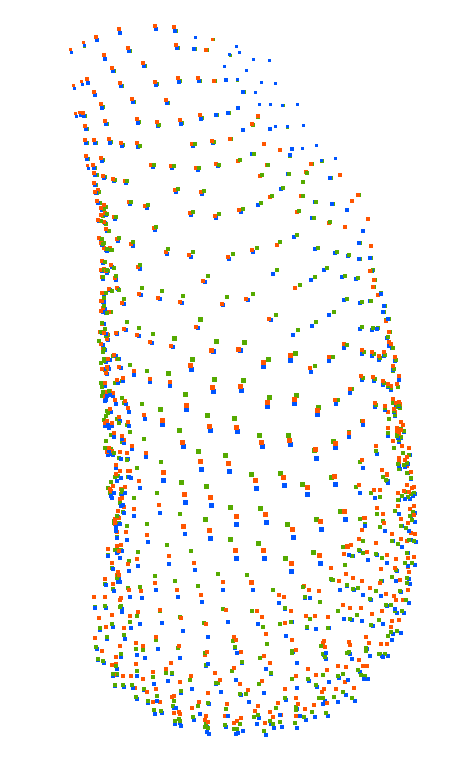
\includegraphics[width = 0.315\textwidth]{naive1_102_cut}\label{fig:naive1_left}} &
\subfloat[Example of a breast with a more noticeable deformation caused by BCS]{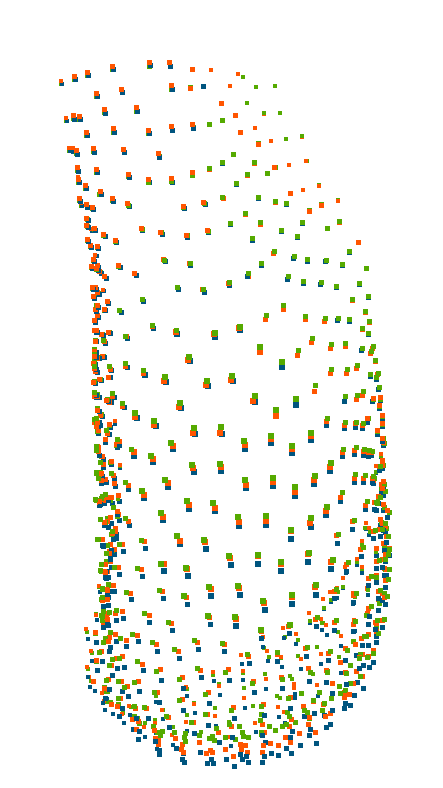
\includegraphics[width = 0.3\textwidth]{naive1_200_cut}\label{fig:naive1_right}}
\end{tabular}
\caption[Comparison between pre-surgical, pos-surgical and predicted through a naive method breast's models]{Comparison between pre-surgical, pos-surgical and predicted through a naive method breast's models. The pre-surgical model is displayed in blue; the pos-surgical models displayed in green, and the naive predicted model displayed in orange.}
\label{fig:naive1}
\end{figure}

The global and local evaluation metrics for the second implementation of the naive method also described in section \ref{sub_sec:naive_method_explanation} are represented respectively in Table \ref{tab:naive2} and Table \ref{tab:naive2_local}. Despite of the improvement on the evaluation metrics, the same effect represent in Figure \ref{fig:naive1} still occurs as shown in Figure \ref{fig:naive2}.

\begin{table}[!htb]
\centering
%\label{tab:naive2}
\begin{tabular}{lll|l|l|l|l|l|l|}
\cline{4-9}
                                                   &                                                                                                             &                                                                       & \textbf{\begin{tabular}[c]{@{}l@{}}predicted\\  to pos\end{tabular}} & \textbf{\begin{tabular}[c]{@{}l@{}}pos to \\ predicted\end{tabular}} & \textbf{pre to pos} & \textbf{pos to pre} & \textbf{\begin{tabular}[c]{@{}l@{}}predicted\\  to pre\end{tabular}} & \textbf{\begin{tabular}[c]{@{}l@{}}pre to \\ predicted\end{tabular}} \\ \hline
\multicolumn{1}{|l|}{\multirow{3}{*}{\textbf{3D}}} & \multicolumn{1}{l|}{\multirow{2}{*}{\textbf{\begin{tabular}[c]{@{}l@{}}Euclidean\\ Distance\end{tabular}}}} & \textbf{Mean}                                                         & 1.523                                                                & 1.503                                                                & 1.758               & 1.731               & 1.414                                                                & 1.415                                                                \\ \cline{3-9} 
\multicolumn{1}{|l|}{}                             & \multicolumn{1}{l|}{}                                                                                       & \textbf{\begin{tabular}[c]{@{}l@{}}Standard\\ Deviation\end{tabular}} & 1.194                                                                & 1.129                                                                & 1.333               & 1.277               & 1.067                                                                & 1.069                                                                \\ \cline{2-9} 
\multicolumn{1}{|l|}{}                             & \multicolumn{2}{l|}{\textbf{Hausdorff Distance}}                                                                                                                                    & 5.327                                                                & 5.137                                                                & 6.513               & 6.317               & 2.939                                                                & 2.939                                                                \\ \hline
\multicolumn{1}{|l|}{\multirow{3}{*}{\textbf{1D}}} & \multicolumn{1}{l|}{\multirow{2}{*}{\textbf{\begin{tabular}[c]{@{}l@{}}Euclidean\\ Distance\end{tabular}}}} & \textbf{Mean}                                                         & 0.127                                                                & 0.113                                                                & 0.160               & 0.110               & 0.073                                                                & 0.090                                                                \\ \cline{3-9} 
\multicolumn{1}{|l|}{}                             & \multicolumn{1}{l|}{}                                                                                       & \textbf{\begin{tabular}[c]{@{}l@{}}Standard\\ Deviation\end{tabular}} & 0.194                                                                & 0.120                                                                & 0.346               & 0.110               & 0.101                                                                & 0.193                                                                \\ \cline{2-9} 
\multicolumn{1}{|l|}{}                             & \multicolumn{2}{l|}{\textbf{Hausdorff Distance}}                                                                                                                                    & 1.685                                                                & 0.851                                                                & 3.168               & 0.704               & 0.618                                                                & 2.091                                                                \\ \hline
\end{tabular}
\caption{Global Evaluation Metrics for the second approach of the naive method}
\label{tab:naive2}
\end{table}

\begin{table}[!htb]
\centering
%\label{tab:naive2_local}
\begin{tabular}{lll|l|l|l|}
\cline{4-6}
                                                   &                                                                                                             &                                                                       & \textbf{\begin{tabular}[c]{@{}l@{}}predicted\\  to pos\end{tabular}} & \textbf{pre to pos} & \textbf{\begin{tabular}[c]{@{}l@{}}predicted\\  to pre\end{tabular}} \\ \hline
\multicolumn{1}{|l|}{\multirow{3}{*}{\textbf{3D}}} & \multicolumn{1}{l|}{\multirow{2}{*}{\textbf{\begin{tabular}[c]{@{}l@{}}Euclidean\\ Distance\end{tabular}}}} & \textbf{Mean}                                                         & 1.634                                                                & 2.206               & 1.723                                                                \\ \cline{3-6} 
\multicolumn{1}{|l|}{}                             & \multicolumn{1}{l|}{}                                                                                       & \textbf{\begin{tabular}[c]{@{}l@{}}Standard\\ Deviation\end{tabular}} & 1.497                                                                & 1.920               & 1.124                                                                \\ \cline{2-6} 
\multicolumn{1}{|l|}{}                             & \multicolumn{2}{l|}{\textbf{Hausdorff Distance}}                                                                                                                                    & 5.763                                                                & 8.410               & 3.152                                                                \\ \hline
\multicolumn{1}{|l|}{\multirow{3}{*}{\textbf{1D}}} & \multicolumn{1}{l|}{\multirow{2}{*}{\textbf{\begin{tabular}[c]{@{}l@{}}Euclidean\\ Distance\end{tabular}}}} & \textbf{Mean}                                                         & 1.231                                                                & 1.904               & 1.397                                                                \\ \cline{3-6} 
\multicolumn{1}{|l|}{}                             & \multicolumn{1}{l|}{}                                                                                       & \textbf{\begin{tabular}[c]{@{}l@{}}Standard\\ Deviation\end{tabular}} & 1.055                                                                & 1.929               & 0.924                                                                \\ \cline{2-6} 
\multicolumn{1}{|l|}{}                             & \multicolumn{2}{l|}{\textbf{Hausdorff Distance}}                                                                                                                                    & 5.174                                                                & 8.092               & 5.191                                                                \\ \hline
\end{tabular}
\caption{Local Evaluation Metrics for the second approach of the naive method}
\label{tab:naive2_local}
\end{table}

\begin{figure}[!htb]
\centering
\begin{tabular}{cc}
\subfloat[Example of a breast with a lesser deformation caused by BCS]{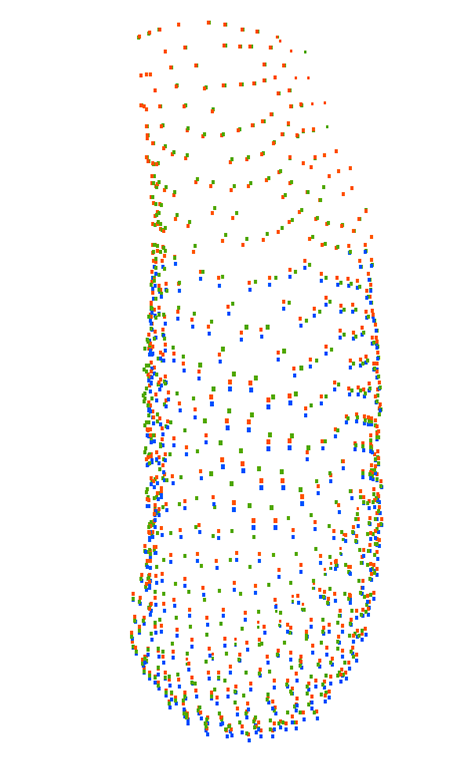
\includegraphics[width = 0.315\textwidth]{naive2_102_cut}\label{fig:naive2_left}} &
\subfloat[Example of a breast with a more noticeable deformation caused by BCS]{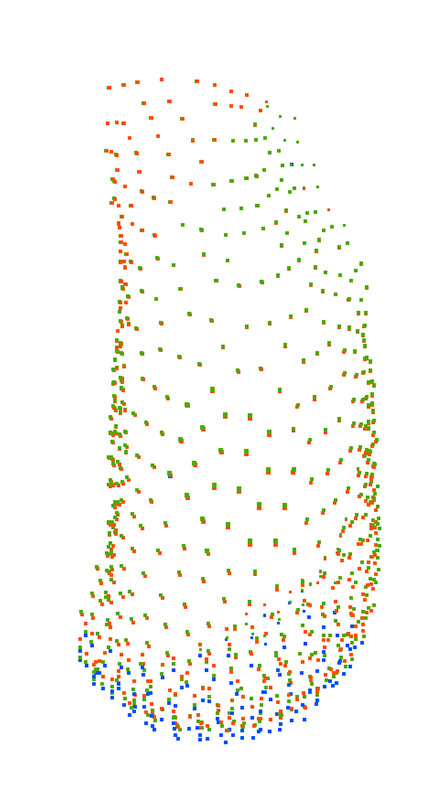
\includegraphics[width = 0.3\textwidth]{naive2_200_cut}\label{fig:naive2_right}}
\end{tabular}
\caption[Comparison between pre-surgical, pos-surgical and predicted breast's models through the second implementation of a naive method ]{Comparison between pre-surgical, pos-surgical and predicted through a naive method breast's models. The pre-surgical model is displayed in blue; the pos-surgical model is displayed in green, and the naive predicted model is displayed in orange.}
\label{fig:naive2}
\end{figure}

\section{Machine Learning Results} \label{sec:ml_results}

The different algorithms described in section \ref{subsec:implementation} were used to train the several prediction models.

The following sections present the results for each ML algorithm in order to understand what led to a better prediction, as well as the features and labels that should be used on each case.

\subsection{Random Forest Results} \label{subsec:rf_results}

In order to predict the displacement of the breast's surface points using RF, three different models were built: one for each axis. Despite of the 3 models, the evaluation was done considering the simultaneous outcome of the three models.

On an initial approach, only considering the surface points in order to train the models, features such the points' coordinates, the distance from the point to the tumor's center of mass, the breast's volume, the tumor's volume and the remaining clinical features as dummy variables. as the points were considered. Another trials were carried out, where the features were represented differently or even omitted. On one of those trials, instead of using the breast's laterality as a categorical variable, the right breast were reflected and considered left breast, leading to worse results in terms of a more inaccurate displacement prediction.

Both global and local evaluation metrics are respectively displayed in Table \ref{tab:rf_loo_g} and Table \ref{tab:rf_loo_l} for the LOO train/test splitting and in Table \ref{tab:rf_biased_g} and Table \ref{tab:rf_biased_l} for the biased train/test split. The biased split (as described in section \ref{subsec:labels}) was constructed by randomly splitting the dataset cases into train and test sets. Since all the cases in the dataset were generated from 6 initial real patients, there is a great probability of a case in the test set having a very similar cases on the training set. By using this is possible to represent an ideal situation of the breast's deformation prediction and understand the results of the best case scenario of the prediction model.


\begin{table}[!htb]
\centering
\begin{tabular}{lll|l|l|l|l|l|l|}
\cline{4-9}
                                                   &                                                                                                             &                                                                       & \textbf{\begin{tabular}[c]{@{}l@{}}predicted\\  to pos\end{tabular}} & \textbf{\begin{tabular}[c]{@{}l@{}}pos to \\ predicted\end{tabular}} & \textbf{pre to pos} & \textbf{pos to pre} & \textbf{\begin{tabular}[c]{@{}l@{}}predicted\\  to pre\end{tabular}} & \textbf{\begin{tabular}[c]{@{}l@{}}pre to \\ predicted\end{tabular}} \\ \hline
\multicolumn{1}{|l|}{\multirow{3}{*}{\textbf{3D}}} & \multicolumn{1}{l|}{\multirow{2}{*}{\textbf{\begin{tabular}[c]{@{}l@{}}Euclidean\\ Distance\end{tabular}}}} & \textbf{Mean}                                                         & 1.103                                                                & 1.102                                                                & 1.758               & 1.731               & 1.848                                                                & 1.866                                                                \\ \cline{3-9} 
\multicolumn{1}{|l|}{}                             & \multicolumn{1}{l|}{}                                                                                       & \textbf{\begin{tabular}[c]{@{}l@{}}Standard\\ Deviation\end{tabular}} & 0.811                                                                & 0.810                                                                & 1.333               & 1.277               & 1.228                                                                & 1.266                                                                \\ \cline{2-9} 
\multicolumn{1}{|l|}{}                             & \multicolumn{2}{l|}{\textbf{Hausdorff Distance}}                                                                                                                                    & 4.062                                                                & 4.031                                                                & 6.513               & 6.317               & 5.580                                                                & 5.738                                                                \\ \hline
\multicolumn{1}{|l|}{\multirow{3}{*}{\textbf{1D}}} & \multicolumn{1}{l|}{\multirow{2}{*}{\textbf{\begin{tabular}[c]{@{}l@{}}Euclidean\\ Distance\end{tabular}}}} & \textbf{Mean}                                                         & 0.105                                                                & 0.104                                                                & 0.160               & 0.110               & 0.119                                                                & 0.158                                                                \\ \cline{3-9} 
\multicolumn{1}{|l|}{}                             & \multicolumn{1}{l|}{}                                                                                       & \textbf{\begin{tabular}[c]{@{}l@{}}Standard\\ Deviation\end{tabular}} & 0.117                                                                & 0.113                                                                & 0.346               & 0.110               & 0.116                                                                & 0.313                                                                \\ \cline{2-9} 
\multicolumn{1}{|l|}{}                             & \multicolumn{2}{l|}{\textbf{Hausdorff Distance}}                                                                                                                                    & 0.970                                                                & 0.875                                                                & 3.168               & 0.704               & 0.714                                                                & 3.049                                                                \\ \hline
\end{tabular}
\caption{Global Evaluation Metrics for RF models using LOO train/test split}
\label{tab:rf_loo_g}
\end{table}

\begin{table}[!htb]
\centering
\begin{tabular}{lll|l|l|l|}
\cline{4-6}
                                                   &                                                                                                             &                                                                       & \textbf{\begin{tabular}[c]{@{}l@{}}predicted\\  to pos\end{tabular}} & \textbf{pre to pos} & \textbf{\begin{tabular}[c]{@{}l@{}}predicted\\  to pre\end{tabular}} \\ \hline
\multicolumn{1}{|l|}{\multirow{3}{*}{\textbf{3D}}} & \multicolumn{1}{l|}{\multirow{2}{*}{\textbf{\begin{tabular}[c]{@{}l@{}}Euclidean\\ Distance\end{tabular}}}} & \textbf{Mean}                                                         & 1.151                                                                & 2.206               & 2.190                                                                \\ \cline{3-6} 
\multicolumn{1}{|l|}{}                             & \multicolumn{1}{l|}{}                                                                                       & \textbf{\begin{tabular}[c]{@{}l@{}}Standard\\ Deviation\end{tabular}} & 0.899                                                                & 1.920               & 1.643                                                                \\ \cline{2-6} 
\multicolumn{1}{|l|}{}                             & \multicolumn{2}{l|}{\textbf{Hausdorff Distance}}                                                                                                                                    & 4.464                                                                & 8.410               & 6.502                                                                \\ \hline
\multicolumn{1}{|l|}{\multirow{3}{*}{\textbf{1D}}} & \multicolumn{1}{l|}{\multirow{2}{*}{\textbf{\begin{tabular}[c]{@{}l@{}}Euclidean\\ Distance\end{tabular}}}} & \textbf{Mean}                                                         & 0.909                                                                & 1.904               & 1.979                                                                \\ \cline{3-6} 
\multicolumn{1}{|l|}{}                             & \multicolumn{1}{l|}{}                                                                                       & \textbf{\begin{tabular}[c]{@{}l@{}}Standard\\ Deviation\end{tabular}} & 0.931                                                                & 1.929               & 1.578                                                                \\ \cline{2-6} 
\multicolumn{1}{|l|}{}                             & \multicolumn{2}{l|}{\textbf{Hausdorff Distance}}                                                                                                                                    & 4.383                                                                & 8.092               & 5.907                                                                \\ \hline
\end{tabular}
\caption{Local Evaluation Metrics for RF models using LOO train/test split}
\label{tab:rf_loo_l}
\end{table}


\begin{table}[!htb]
\centering
\begin{tabular}{lll|l|l|l|l|l|l|}
\cline{4-9}
                                                   &                                                                                                             &                                                                       & \textbf{\begin{tabular}[c]{@{}l@{}}predicted\\  to pos\end{tabular}} & \textbf{\begin{tabular}[c]{@{}l@{}}pos to \\ predicted\end{tabular}} & \textbf{pre to pos} & \textbf{pos to pre} & \textbf{\begin{tabular}[c]{@{}l@{}}predicted\\  to pre\end{tabular}} & \textbf{\begin{tabular}[c]{@{}l@{}}pre to \\ predicted\end{tabular}} \\ \hline
\multicolumn{1}{|l|}{\multirow{3}{*}{\textbf{3D}}} & \multicolumn{1}{l|}{\multirow{2}{*}{\textbf{\begin{tabular}[c]{@{}l@{}}Euclidean\\ Distance\end{tabular}}}} & \textbf{Mean}                                                         & 0.674                                                                & 0.672                                                                & 1.799               & 1.773               & 1.772                                                                & 1.784                                                                \\ \cline{3-9} 
\multicolumn{1}{|l|}{}                             & \multicolumn{1}{l|}{}                                                                                       & \textbf{\begin{tabular}[c]{@{}l@{}}Standard\\ Deviation\end{tabular}} & 0.600                                                                & 0.597                                                                & 1.379               & 1.325               & 1.236                                                                & 1.262                                                                \\ \cline{2-9} 
\multicolumn{1}{|l|}{}                             & \multicolumn{2}{l|}{\textbf{Hausdorff Distance}}                                                                                                                                    & 3.199                                                                & 3.127                                                                & 6.550               & 6.326               & 5.398                                                                & 5.539                                                                \\ \hline
\multicolumn{1}{|l|}{\multirow{3}{*}{\textbf{1D}}} & \multicolumn{1}{l|}{\multirow{2}{*}{\textbf{\begin{tabular}[c]{@{}l@{}}Euclidean\\ Distance\end{tabular}}}} & \textbf{Mean}                                                         & 0.096                                                                & 0.096                                                                & 0.162               & 0.111               & 0.119                                                                & 0.160                                                                \\ \cline{3-9} 
\multicolumn{1}{|l|}{}                             & \multicolumn{1}{l|}{}                                                                                       & \textbf{\begin{tabular}[c]{@{}l@{}}Standard\\ Deviation\end{tabular}} & 0.103                                                                & 0.102                                                                & 0.349               & 0.111               & 0.116                                                                & 0.328                                                                \\ \cline{2-9} 
\multicolumn{1}{|l|}{}                             & \multicolumn{2}{l|}{\textbf{Hausdorff Distance}}                                                                                                                                    & 0.781                                                                & 0.761                                                                & 3.274               & 0.718               & 0.725                                                                & 3.238                                                                \\ \hline
\end{tabular}
\caption{Global Evaluation Metrics for RF models using the train/test biased split}
\label{tab:rf_biased_g}
\end{table}

\begin{table}[!htb]
\centering
\begin{tabular}{lll|l|l|l|}
\cline{4-6}
                                                   &                                                                                                             &                                                                       & \textbf{\begin{tabular}[c]{@{}l@{}}predicted\\  to pos\end{tabular}} & \textbf{pre to pos} & \textbf{\begin{tabular}[c]{@{}l@{}}predicted\\  to pre\end{tabular}} \\ \hline
\multicolumn{1}{|l|}{\multirow{3}{*}{\textbf{3D}}} & \multicolumn{1}{l|}{\multirow{2}{*}{\textbf{\begin{tabular}[c]{@{}l@{}}Euclidean\\ Distance\end{tabular}}}} & \textbf{Mean}                                                         & 0.680                                                                & 2.196               & 2.096                                                                \\ \cline{3-6} 
\multicolumn{1}{|l|}{}                             & \multicolumn{1}{l|}{}                                                                                       & \textbf{\begin{tabular}[c]{@{}l@{}}Standard\\ Deviation\end{tabular}} & 0.615                                                                & 1.917               & 1.636                                                                \\ \cline{2-6} 
\multicolumn{1}{|l|}{}                             & \multicolumn{2}{l|}{\textbf{Hausdorff Distance}}                                                                                                                                    & 3.256                                                                & 8.337               & 6.448                                                                \\ \hline
\multicolumn{1}{|l|}{\multirow{3}{*}{\textbf{1D}}} & \multicolumn{1}{l|}{\multirow{2}{*}{\textbf{\begin{tabular}[c]{@{}l@{}}Euclidean\\ Distance\end{tabular}}}} & \textbf{Mean}                                                         & 0.643                                                                & 2.115               & 2.032                                                                \\ \cline{3-6} 
\multicolumn{1}{|l|}{}                             & \multicolumn{1}{l|}{}                                                                                       & \textbf{\begin{tabular}[c]{@{}l@{}}Standard\\ Deviation\end{tabular}} & 0.730                                                                & 2.115               & 1.719                                                                \\ \cline{2-6} 
\multicolumn{1}{|l|}{}                             & \multicolumn{2}{l|}{\textbf{Hausdorff Distance}}                                                                                                                                    & 3.777                                                                & 8.728               & 6.483                                                                \\ \hline
\end{tabular}
\caption{Local Evaluation Metrics for RF models using the train/test biased split}
\label{tab:rf_biased_l}
\end{table}

In order to train the models, whose results were previously presented, were trained using an automatic model tuning \footnote{\url{http://machinelearningmastery.com/tuning-machine-learning-models-using-the-caret-r-package/}}, that tries to find the best parametrization of the model to the problem. In the presented case, the model parameters were as follows: \textit{$mtry=8$}; \textit{$n\_trees=250$}; \textit{$node\_size=1$}. \textit{n\_trees} represents the number of decision trees used for training the model, \textit{mtry} represents the number of variables sampled at each split, and \textit{node\_size} represents the minimum size of terminal nodes on the model. \footnote{\url{https://www.rdocumentation.org/packages/randomForest/versions/4.6-12/topics/randomForest}}.
The feature importance computed by these models is also represented in Table \ref{tab:rf_feature_imp} and the visual results are presented in Figure \ref{fig:rf_visual}.

\begin{table}[!htb]
\centering
\begin{tabular}{l|lll}
\textbf{Features} & \textbf{$\partial$x} & \textbf{$\partial$y}   & \textbf{$\partial$z}   \\ \hline
x\_coord          & 48.10         & 55.22  & 76.37  \\ \hline
y\_coord          & 74.93         & 101.35 & 78.38  \\ \hline
z\_coord          & 85.16         & 71.69  & 35.85  \\ \hline
x\_diff           & 82.15         & 60.54  & 85.77  \\ \hline
y\_diff           & 56.29         & 71.69  & 61.87  \\ \hline
z\_diff           & 73.54         & 127.16 & 59.96  \\ \hline
dist              & 57.78         & 58.70  & 45.61  \\ \hline
b\_vol            & 25.08         & 40.52 & 59.92 \\ \hline
t\_vol            & 103.19        & 132.59 & 168.23 \\ \hline
lat\_a            & 18.07         & 12.85  & 26.63 \\ \hline
lat\_b            & 17.41         & 13.38  & 26.88 \\ \hline
acr\_a            & 25.58         & 27.89  & 27.64  \\ \hline
acr\_b            & 28.95         & 23.58  & 20.25  \\ \hline
acr\_c            & 30.48         & 23.95  & 24.78  \\ \hline
acr\_d            & 30.69         & 19.70  & 22.73  \\ \hline
reg\_a            & 27.22         & 21.95  & 12.76  \\ \hline
reg\_b            & 28.24         & 28.29  & 22.37  \\ \hline
reg\_c            & 29.95         & 23.56  & 17.61  \\ \hline
reg\_d            & 41.45         & 22.98  & 27.28 
\end{tabular}
\caption{RF feature importance}
\label{tab:rf_feature_imp}
\end{table}

\begin{figure}[!htb]
\centering
\scalebox{0.6}{%
\begin{tabular}{cc}
\subfloat[]{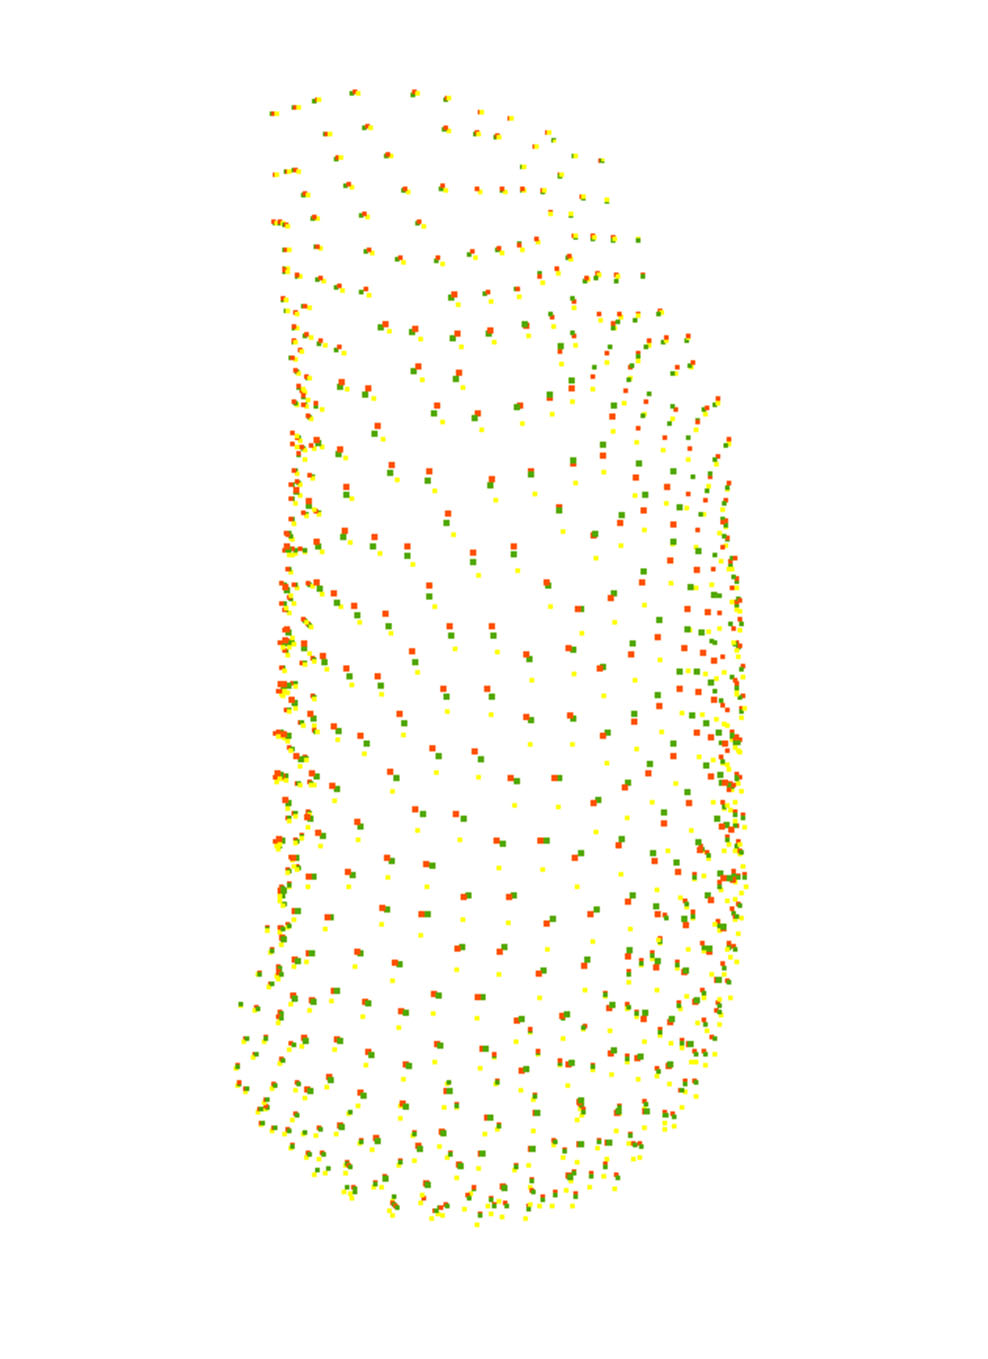
\includegraphics[width = 3in]{visual_pat1}} &
\subfloat[]{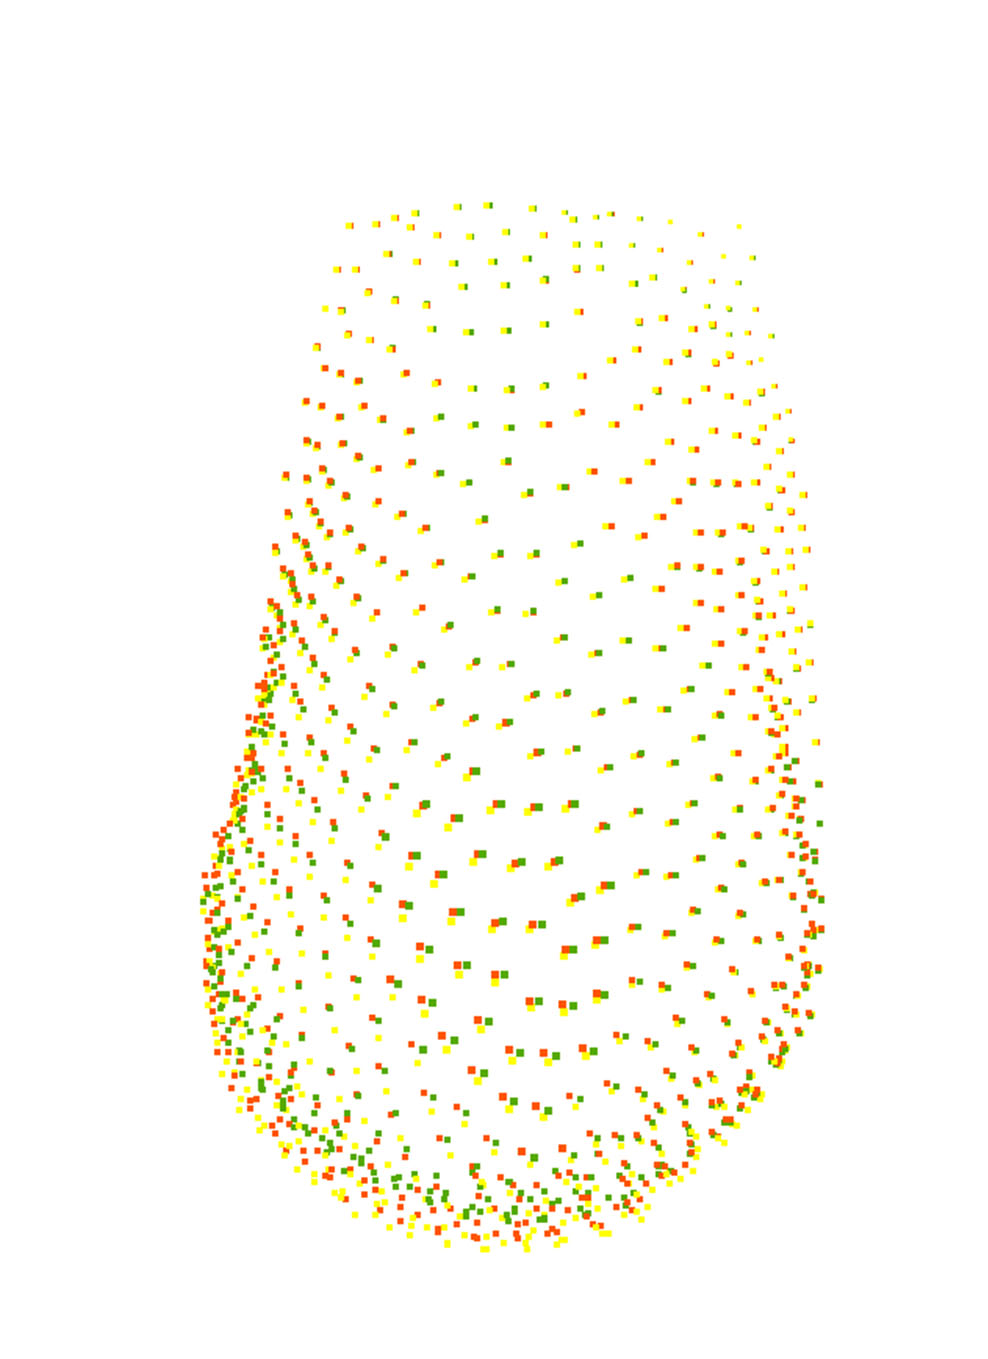
\includegraphics[width = 3in]{visual_pat2}}\\
\subfloat[]{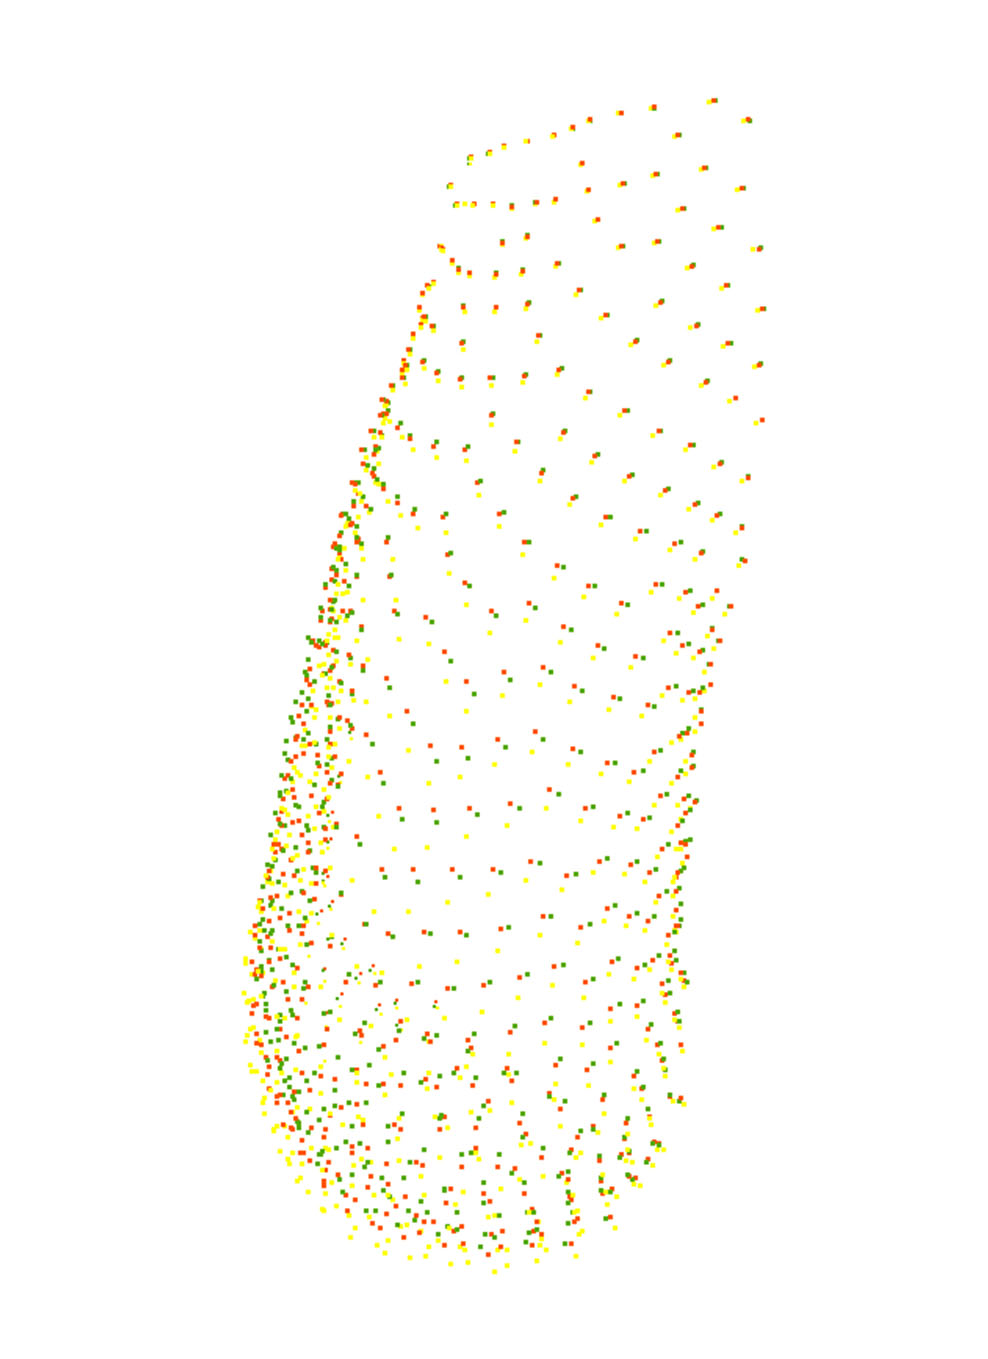
\includegraphics[width = 3in]{visual_pat3}} &
\subfloat[]{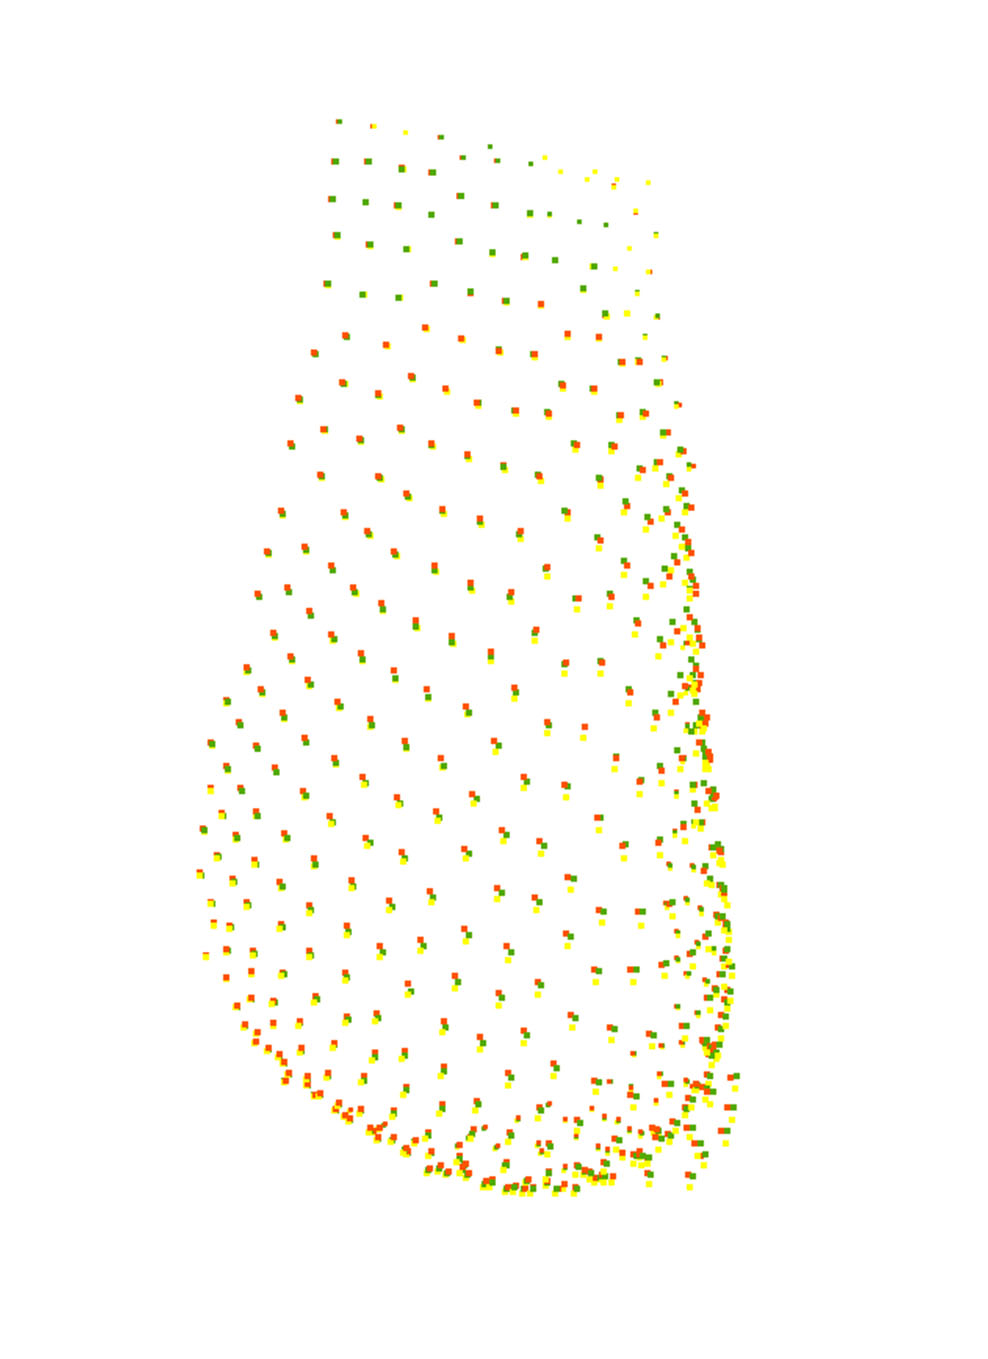
\includegraphics[width = 3in]{visual_pat4}}\\
\subfloat[]{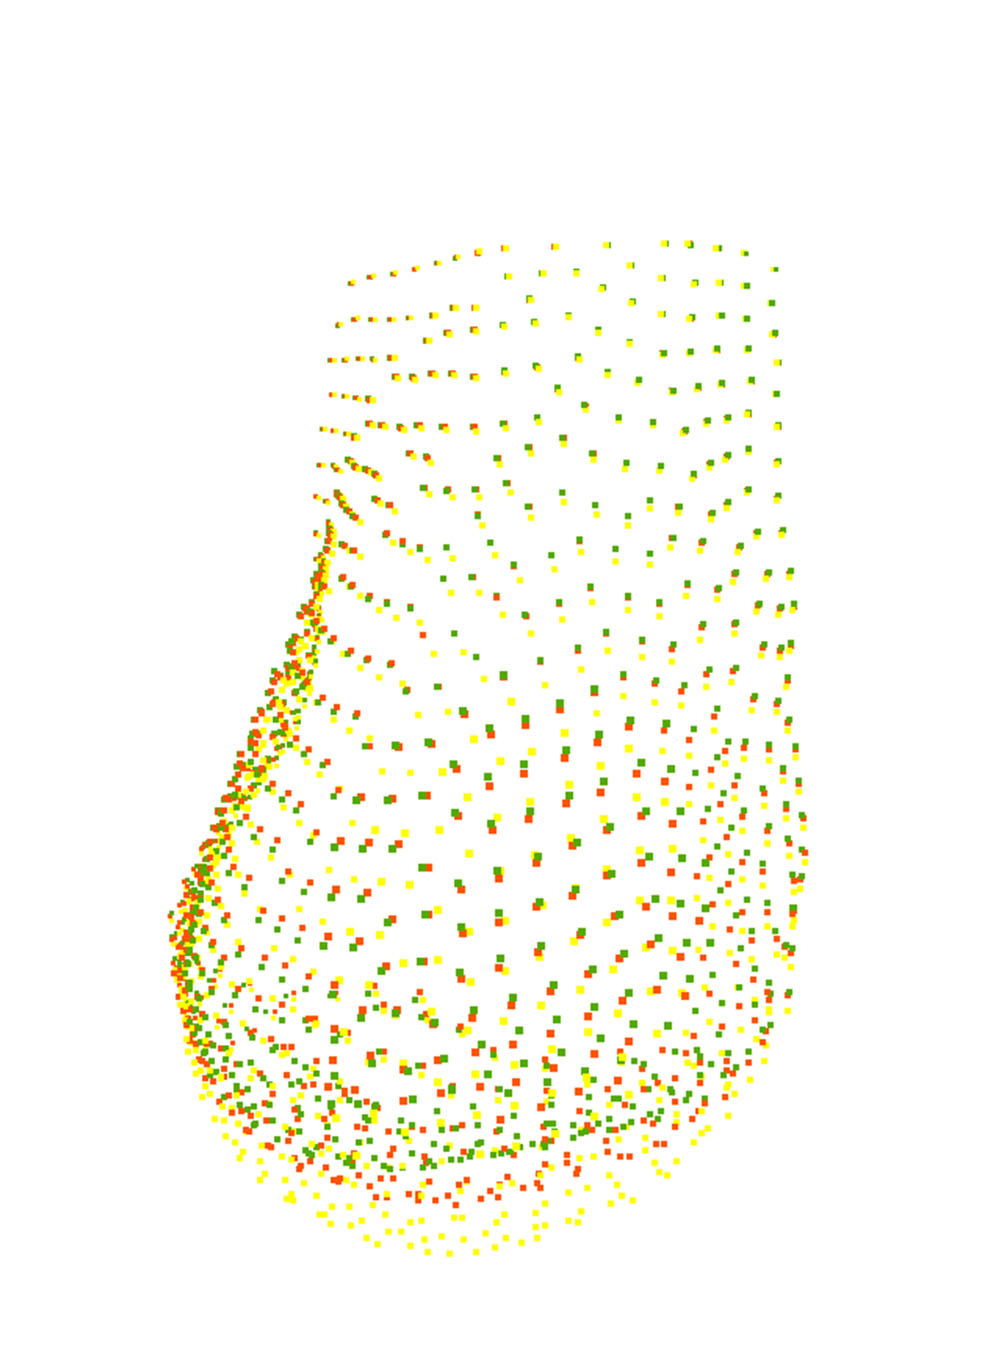
\includegraphics[width = 3in]{visual_pat5}} &
\subfloat[]{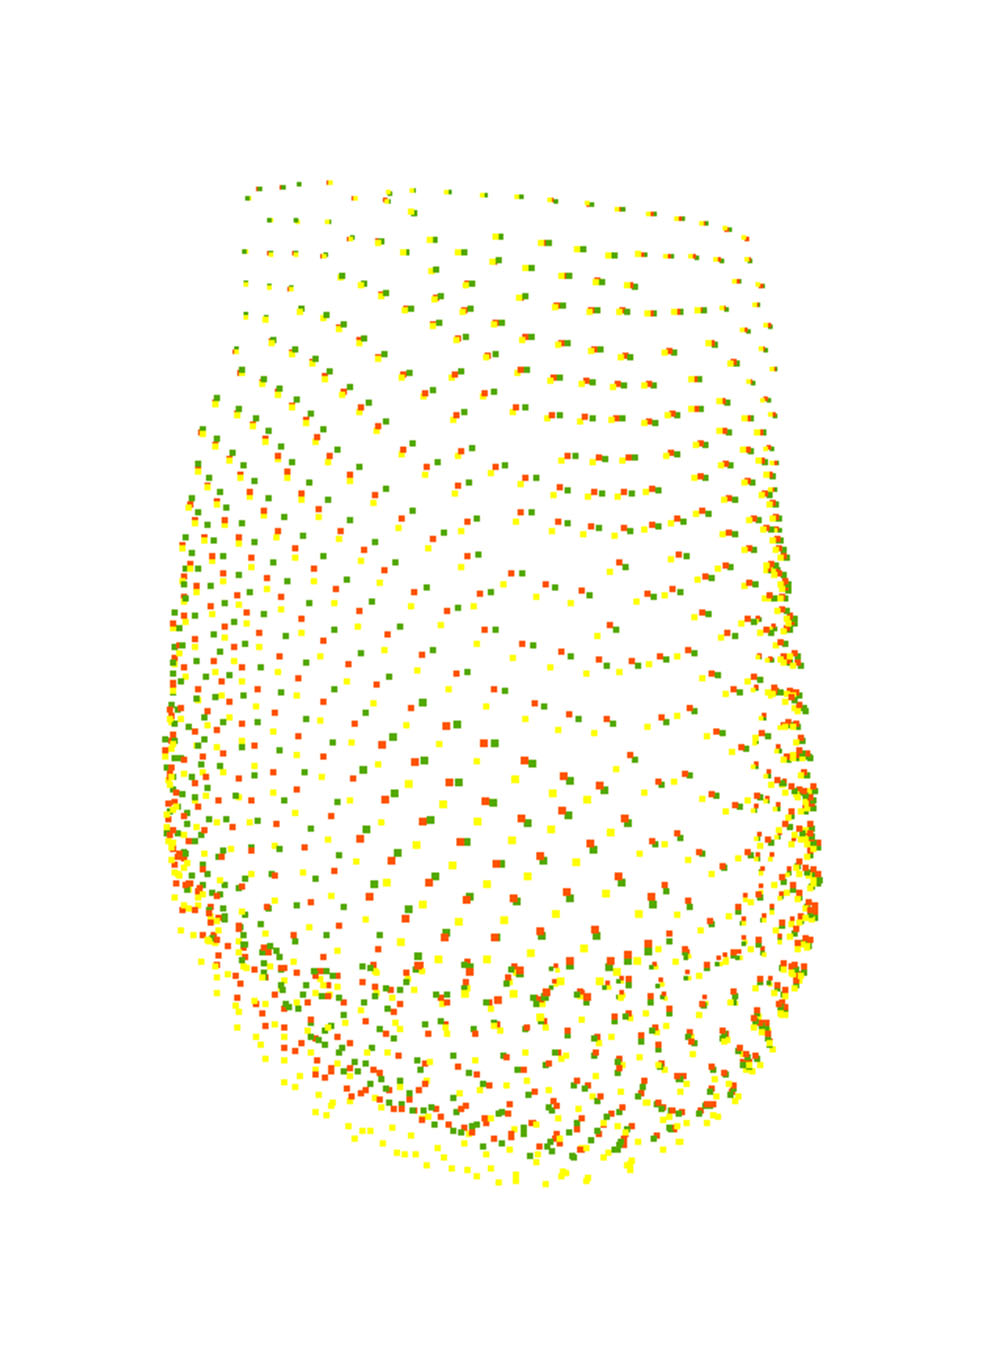
\includegraphics[width = 3in]{visual_pat6}}
\end{tabular}
}
\caption[Visual examples of the prediction results obtained by the RF prediction models]{Visual examples of the prediction results obtained by the RF prediction models. The pre-surgical model is displayed in yellow; the pos-surgical model is displayed in green; The predicted model is displayed in red.}
\label{fig:rf_visual}
\end{figure}

Despite of the previous scenario only considered the surface points of the patient's breast models, using additional points such as internal points, can lead to a better prediction of the deformation. The internal points were only used to train the model. The global and local distance metrics for this scenario are respectively shown in Table \ref{tab:rf_si_loo_g} and Table \ref{tab:rf_si_loo_l}. These results were achieved by using the LOO split and the same model parameters. The evaluation metrics regarding the results of the models trained with both surface and internal points, with the biased split are described in Table \ref{tab:rf_si_biased_g} and Table \ref{tab:rf_si_biased_l}.

\begin{table}[!htb]
\centering
\begin{tabular}{lll|l|l|l|l|l|l|}
\cline{4-9}
                                                   &                                                                                                             &                                                                       & \textbf{\begin{tabular}[c]{@{}l@{}}predicted\\  to pos\end{tabular}} & \textbf{\begin{tabular}[c]{@{}l@{}}pos to \\ predicted\end{tabular}} & \textbf{pre to pos} & \textbf{pos to pre} & \textbf{\begin{tabular}[c]{@{}l@{}}predicted\\  to pre\end{tabular}} & \textbf{\begin{tabular}[c]{@{}l@{}}pre to \\ predicted\end{tabular}} \\ \hline
\multicolumn{1}{|l|}{\multirow{3}{*}{\textbf{3D}}} & \multicolumn{1}{l|}{\multirow{2}{*}{\textbf{\begin{tabular}[c]{@{}l@{}}Euclidean\\ Distance\end{tabular}}}} & \textbf{Mean}                                                         & 1.044                                                                & 1.043                                                                & 1.555               & 1.529               & 1.652                                                                & 1.670                                                                \\ \cline{3-9} 
\multicolumn{1}{|l|}{}                             & \multicolumn{1}{l|}{}                                                                                       & \textbf{\begin{tabular}[c]{@{}l@{}}Standard\\ Deviation\end{tabular}} & 0.840                                                                & 0.837                                                                & 1.382               & 1.319               & 1.257                                                                & 1.296                                                                \\ \cline{2-9} 
\multicolumn{1}{|l|}{}                             & \multicolumn{2}{l|}{\textbf{Hausdorff Distance}}                                                                                                                                    & 4.875                                                                & 4.817                                                                & 7.107               & 6.406               & 5.533                                                                & 5.923                                                                \\ \hline
\multicolumn{1}{|l|}{\multirow{3}{*}{\textbf{1D}}} & \multicolumn{1}{l|}{\multirow{2}{*}{\textbf{\begin{tabular}[c]{@{}l@{}}Euclidean\\ Distance\end{tabular}}}} & \textbf{Mean}                                                         & 0.055                                                                & 0.055                                                                & 0.080               & 0.055               & 0.060                                                                & 0.083                                                                \\ \cline{3-9} 
\multicolumn{1}{|l|}{}                             & \multicolumn{1}{l|}{}                                                                                       & \textbf{\begin{tabular}[c]{@{}l@{}}Standard\\ Deviation\end{tabular}} & 0.063                                                                & 0.068                                                                & 0.236               & 0.060               & 0.062                                                                & 0.238                                                                \\ \cline{2-9} 
\multicolumn{1}{|l|}{}                             & \multicolumn{2}{l|}{\textbf{Hausdorff Distance}}                                                                                                                                    & 0.659                                                                & 0.789                                                                & 3.154               & 0.477               & 0.465                                                                & 3.287                                                                \\ \hline
\end{tabular}
\caption{Global Evaluation Metrics for RF models considering breast internal points with LOO train/test split}
\label{tab:rf_si_loo_g}
\end{table}


\begin{table}[!htb]
\centering
\begin{tabular}{lll|l|l|l|}
\cline{4-6}
                                                   &                                                                                                             &                                                                       & \textbf{\begin{tabular}[c]{@{}l@{}}predicted\\  to pos\end{tabular}} & \textbf{pre to pos} & \textbf{\begin{tabular}[c]{@{}l@{}}predicted\\  to pre\end{tabular}} \\ \hline
\multicolumn{1}{|l|}{\multirow{3}{*}{\textbf{3D}}} & \multicolumn{1}{l|}{\multirow{2}{*}{\textbf{\begin{tabular}[c]{@{}l@{}}Euclidean\\ Distance\end{tabular}}}} & \textbf{Mean}                                                         & 1.077                                                                & 1.919               & 1.912                                                                \\ \cline{3-6} 
\multicolumn{1}{|l|}{}                             & \multicolumn{1}{l|}{}                                                                                       & \textbf{\begin{tabular}[c]{@{}l@{}}Standard\\ Deviation\end{tabular}} & 0.911                                                                & 1.940               & 1.611                                                                \\ \cline{2-6} 
\multicolumn{1}{|l|}{}                             & \multicolumn{2}{l|}{\textbf{Hausdorff Distance}}                                                                                                                                    & 5.352                                                                & 9.510               & 6.620                                                                \\ \hline
\multicolumn{1}{|l|}{\multirow{3}{*}{\textbf{1D}}} & \multicolumn{1}{l|}{\multirow{2}{*}{\textbf{\begin{tabular}[c]{@{}l@{}}Euclidean\\ Distance\end{tabular}}}} & \textbf{Mean}                                                         & 0.817                                                                & 1.693               & 1.759                                                                \\ \cline{3-6} 
\multicolumn{1}{|l|}{}                             & \multicolumn{1}{l|}{}                                                                                       & \textbf{\begin{tabular}[c]{@{}l@{}}Standard\\ Deviation\end{tabular}} & 0.889                                                                & 1.908               & 1.620                                                                \\ \cline{2-6} 
\multicolumn{1}{|l|}{}                             & \multicolumn{2}{l|}{\textbf{Hausdorff Distance}}                                                                                                                                    & 5.003                                                                & 9.147               & 6.475                                                                \\ \hline
\end{tabular}
\caption{Local Evaluation Metrics for RF models considering breast internal points with LOO train/test split}
\label{tab:rf_si_loo_l}
\end{table}


\begin{table}[!htb]
\centering
\begin{tabular}{lll|l|l|l|l|l|l|}
\cline{4-9}
                                                   &                                                                                                             &                                                                       & \textbf{\begin{tabular}[c]{@{}l@{}}predicted\\  to pos\end{tabular}} & \textbf{\begin{tabular}[c]{@{}l@{}}pos to \\ predicted\end{tabular}} & \textbf{pre to pos} & \textbf{pos to pre} & \textbf{\begin{tabular}[c]{@{}l@{}}predicted\\  to pre\end{tabular}} & \textbf{\begin{tabular}[c]{@{}l@{}}pre to \\ predicted\end{tabular}} \\ \hline
\multicolumn{1}{|l|}{\multirow{3}{*}{\textbf{3D}}} & \multicolumn{1}{l|}{\multirow{2}{*}{\textbf{\begin{tabular}[c]{@{}l@{}}Euclidean\\ Distance\end{tabular}}}} & \textbf{Mean}                                                         & 0.639                                                                & 0.638                                                                & 1.592               & 1.562               & 1.653                                                                & 1.679                                                                \\ \cline{3-9} 
\multicolumn{1}{|l|}{}                             & \multicolumn{1}{l|}{}                                                                                       & \textbf{\begin{tabular}[c]{@{}l@{}}Standard\\ Deviation\end{tabular}} & 0.614                                                                & 0.610                                                                & 1.391               & 1.318               & 1.336                                                                & 1.394                                                                \\ \cline{2-9} 
\multicolumn{1}{|l|}{}                             & \multicolumn{2}{l|}{\textbf{Hausdorff Distance}}                                                                                                                                    & 3.979                                                                & 3.932                                                                & 7.054               & 6.252               & 5.957                                                                & 6.452                                                                \\ \hline
\multicolumn{1}{|l|}{\multirow{3}{*}{\textbf{1D}}} & \multicolumn{1}{l|}{\multirow{2}{*}{\textbf{\begin{tabular}[c]{@{}l@{}}Euclidean\\ Distance\end{tabular}}}} & \textbf{Mean}                                                         & 0.050                                                                & 0.049                                                                & 0.088               & 0.056               & 0.058                                                                & 0.083                                                                \\ \cline{3-9} 
\multicolumn{1}{|l|}{}                             & \multicolumn{1}{l|}{}                                                                                       & \textbf{\begin{tabular}[c]{@{}l@{}}Standard\\ Deviation\end{tabular}} & 0.062                                                                & 0.053                                                                & 0.284               & 0.060               & 0.062                                                                & 0.243                                                                \\ \cline{2-9} 
\multicolumn{1}{|l|}{}                             & \multicolumn{2}{l|}{\textbf{Hausdorff Distance}}                                                                                                                                    & 0.773                                                                & 0.480                                                                & 3.695               & 0.461               & 0.471                                                                & 3.325                                                                \\ \hline
\end{tabular}
\caption{Global Evaluation Metrics for RF models considering breast internal points with random train/test split}
\label{tab:rf_si_biased_g}
\end{table}


\begin{table}[!htb]
\centering
\begin{tabular}{lll|l|l|l|}
\cline{4-6}
                                                   &                                                                                                             &                                                                       & \textbf{\begin{tabular}[c]{@{}l@{}}predicted\\  to pos\end{tabular}} & \textbf{pre to pos} & \textbf{\begin{tabular}[c]{@{}l@{}}predicted\\  to pre\end{tabular}} \\ \hline
\multicolumn{1}{|l|}{\multirow{3}{*}{\textbf{3D}}} & \multicolumn{1}{l|}{\multirow{2}{*}{\textbf{\begin{tabular}[c]{@{}l@{}}Euclidean\\ Distance\end{tabular}}}} & \textbf{Mean}                                                         & 0.644                                                                & 2.019               & 2.001                                                                \\ \cline{3-6} 
\multicolumn{1}{|l|}{}                             & \multicolumn{1}{l|}{}                                                                                       & \textbf{\begin{tabular}[c]{@{}l@{}}Standard\\ Deviation\end{tabular}} & 0.630                                                                & 2.046               & 1.826                                                                \\ \cline{2-6} 
\multicolumn{1}{|l|}{}                             & \multicolumn{2}{l|}{\textbf{Hausdorff Distance}}                                                                                                                                    & 4.090                                                                & 9.927               & 7.420                                                                \\ \hline
\multicolumn{1}{|l|}{\multirow{3}{*}{\textbf{1D}}} & \multicolumn{1}{l|}{\multirow{2}{*}{\textbf{\begin{tabular}[c]{@{}l@{}}Euclidean\\ Distance\end{tabular}}}} & \textbf{Mean}                                                         & 0.501                                                                & 1.732               & 1.631                                                                \\ \cline{3-6} 
\multicolumn{1}{|l|}{}                             & \multicolumn{1}{l|}{}                                                                                       & \textbf{\begin{tabular}[c]{@{}l@{}}Standard\\ Deviation\end{tabular}} & 0.624                                                                & 1.941               & 1.648                                                                \\ \cline{2-6} 
\multicolumn{1}{|l|}{}                             & \multicolumn{2}{l|}{\textbf{Hausdorff Distance}}                                                                                                                                    & 3.870                                                                & 9.190               & 6.710                                                                \\ \hline
\end{tabular}
\caption{Local Evaluation Metrics for RF models considering breast internal points with random train/test split}
\label{tab:rf_si_biased_l}
\end{table}


By comparing the results of the two distinct scenarios previously analysed, it is possible to conclude that considering the internal points of the breast's model leads to better results.


\subsection{Multilayer Perceptron Results} \label{subsec:mlp_results}

In order to try achieving better results other ML algorithms such as MLP were tested. However, unlike RF, other ML algorithms require a prior feature selection in order to achieve reliable values. In case of MLP, a Recursive Feature Elimination \footnote{\url{https://topepo.github.io/caret/recursive-feature-elimination.html}} (RFE) technique was used in order to understand the features to be used on the model training.   

\begin{figure}[!htb]
\begin{center}
    \leavevmode
    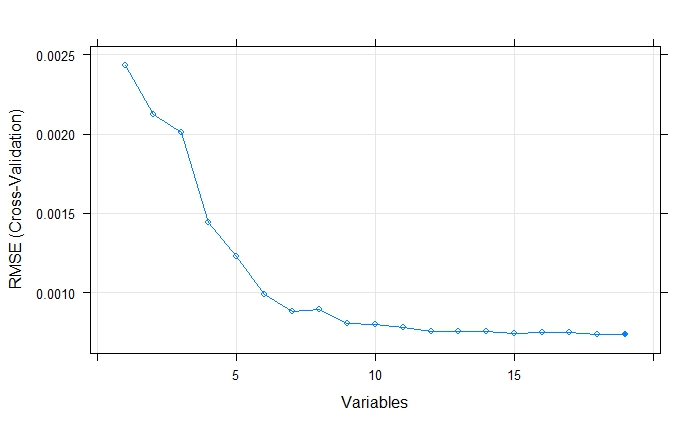
\includegraphics[width=0.9\textwidth]{rfe}
    \caption[aa]{aa}
    \label{fig:rfe}
  \end{center}
\end{figure}

Considering the result of the feature selection, it is possible to conclude that all the features lead to a decrease of the root mean squared error (RMSE), this way, all the feature should be considered when training the model. Given this, a model with the intent of predicting the displacement of the points in the \textit{z} coordinate axis was trained. Its results are compared to the prediction result of RF and represented in Figure \ref{fig:rf_vs_mlp}.

\begin{figure}[!htb]
\begin{center}
	\leavevmode
	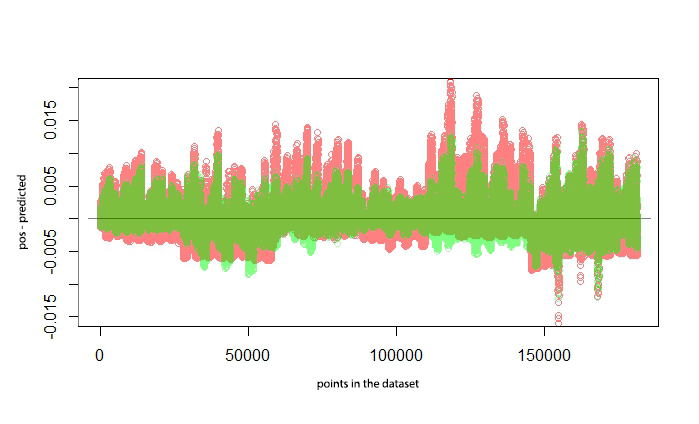
\includegraphics[width=1.0\textwidth]{rf_vs_mlp}
	\caption[Comparison between the predictions of RF and MLP regression models.]{Comparison between the predictions of RF and MLP regression models. The \textit{y} axis represents the distance between the point in the pos-surgical model and the predicted model, in the z axis of the Cartesian coordinate system. The \textit{x} axis represents all the points of the dataset, considering all the 288 patients. The distance relative the RF model is displayed in green, while the distance of the MLP model is displayed in red.}
	\label{fig:rf_vs_mlp}
\end{center}
\end{figure}

As represented in Figure \ref{fig:rf_vs_mlp}, the distance between the pos-surgical and the predicted models of the breast's patients is significantly larger when using MLP instead of RF. 


\subsection{Multi-output Regressor Results} \label{subsec:mor_results}

Given the unsatisfactory results of MLP, the following experiments will be using a more promising algorithm such as Multi-output regression (MOR) algorithms. This type of algorithms usually lead to better results than RF and allow to predict several target variables in the same model, unlike what was done so far that for each axis, a different RF model was used.

Using MOR led to the development of four new scenarios, being all of them tested with both LOO and random train/test splits of the data. With the first and second scenarios, the model tries to predict the displacement of the points in the three axis of the Cartesian coordinate system. In the first scenario, only the surface points of the breast's model were used to train the model. The evaluation metrics regarding this scenario may be found in Table \ref{tab:mor_xyz_s_loo_g} and Table \ref{tab:mor_xyz_s_loo_l}. 

\begin{table}[!htb]
\centering
\begin{tabular}{lll|l|l|l|l|l|l|}
\cline{4-9}
                                                   &                                                                                                             &                                                                       & \textbf{\begin{tabular}[c]{@{}l@{}}predicted\\  to pos\end{tabular}} & \textbf{\begin{tabular}[c]{@{}l@{}}pos to \\ predicted\end{tabular}} & \textbf{pre to pos} & \textbf{pos to pre} & \textbf{\begin{tabular}[c]{@{}l@{}}predicted\\  to pre\end{tabular}} & \textbf{\begin{tabular}[c]{@{}l@{}}pre to \\ predicted\end{tabular}} \\ \hline
\multicolumn{1}{|l|}{\multirow{3}{*}{\textbf{3D}}} & \multicolumn{1}{l|}{\multirow{2}{*}{\textbf{\begin{tabular}[c]{@{}l@{}}Euclidean\\ Distance\end{tabular}}}} & \textbf{Mean}                                                         & 1.227                                                                & 1.225                                                                & 1.758               & 1.731               & 1.934                                                                & 1.950                                                                \\ \cline{3-9} 
\multicolumn{1}{|l|}{}                             & \multicolumn{1}{l|}{}                                                                                       & \textbf{\begin{tabular}[c]{@{}l@{}}Standard\\ Deviation\end{tabular}} & 0.863                                                                & 0.857                                                                & 1.333               & 1.277               & 1.194                                                                & 1.226                                                                \\ \cline{2-9} 
\multicolumn{1}{|l|}{}                             & \multicolumn{2}{l|}{\textbf{Hausdorff Distance}}                                                                                                                                    & 4.336                                                                & 5.280                                                                & 6.513               & 6.317               & 5.382                                                                & 5.555                                                                \\ \hline
\multicolumn{1}{|l|}{\multirow{3}{*}{\textbf{1D}}} & \multicolumn{1}{l|}{\multirow{2}{*}{\textbf{\begin{tabular}[c]{@{}l@{}}Euclidean\\ Distance\end{tabular}}}} & \textbf{Mean}                                                         & 0.114                                                                & 0.114                                                                & 0.160               & 0.110               & 0.127                                                                & 0.173                                                                \\ \cline{3-9} 
\multicolumn{1}{|l|}{}                             & \multicolumn{1}{l|}{}                                                                                       & \textbf{\begin{tabular}[c]{@{}l@{}}Standard\\ Deviation\end{tabular}} & 0.121                                                                & 0.128                                                                & 0.346               & 0.110               & 0.121                                                                & 0.355                                                                \\ \cline{2-9} 
\multicolumn{1}{|l|}{}                             & \multicolumn{2}{l|}{\textbf{Hausdorff Distance}}                                                                                                                                    & 0.939                                                                & 1.096                                                                & 3.168               & 0.704               & 0.747                                                                & 3.403                                                                \\ \hline
\end{tabular}
\caption{Global Evaluation Metrics for MOR model considering only breast surface points to predict the displacement of the points in the three different axis. This results are relative to the LOO train/test split.}
\label{tab:mor_xyz_s_loo_g}
\end{table}

\begin{table}[!htb]
\centering
\begin{tabular}{lll|l|l|l|}
\cline{4-6}
                                                   &                                                                                                             &                                                                       & \textbf{\begin{tabular}[c]{@{}l@{}}predicted\\  to pos\end{tabular}} & \textbf{pre to pos} & \textbf{\begin{tabular}[c]{@{}l@{}}predicted\\  to pre\end{tabular}} \\ \hline
\multicolumn{1}{|l|}{\multirow{3}{*}{\textbf{3D}}} & \multicolumn{1}{l|}{\multirow{2}{*}{\textbf{\begin{tabular}[c]{@{}l@{}}Euclidean\\ Distance\end{tabular}}}} & \textbf{Mean}                                                         & 1.298                                                                & 2.206               & 2.224                                                                \\ \cline{3-6} 
\multicolumn{1}{|l|}{}                             & \multicolumn{1}{l|}{}                                                                                       & \textbf{\begin{tabular}[c]{@{}l@{}}Standard\\ Deviation\end{tabular}} & 0.983                                                                & 1.920               & 1.523                                                                \\ \cline{2-6} 
\multicolumn{1}{|l|}{}                             & \multicolumn{2}{l|}{\textbf{Hausdorff Distance}}                                                                                                                                    & 4.857                                                                & 8.410               & 6.115                                                                \\ \hline
\multicolumn{1}{|l|}{\multirow{3}{*}{\textbf{1D}}} & \multicolumn{1}{l|}{\multirow{2}{*}{\textbf{\begin{tabular}[c]{@{}l@{}}Euclidean\\ Distance\end{tabular}}}} & \textbf{Mean}                                                         & 1.000                                                                & 1.904               & 2.062                                                                \\ \cline{3-6} 
\multicolumn{1}{|l|}{}                             & \multicolumn{1}{l|}{}                                                                                       & \textbf{\begin{tabular}[c]{@{}l@{}}Standard\\ Deviation\end{tabular}} & 0.968                                                                & 1.929               & 1.563                                                                \\ \cline{2-6} 
\multicolumn{1}{|l|}{}                             & \multicolumn{2}{l|}{\textbf{Hausdorff Distance}}                                                                                                                                    & 4.498                                                                & 8.092               & 5.999                                                                \\ \hline
\end{tabular}
\caption{Local Evaluation Metrics for MOR model considering only breast surface points to predict the displacement of the points in the three different axis. This results are relative to the LOO train/test split.}
\label{tab:mor_xyz_s_loo_l}
\end{table}


The second scenario was trained in the same condition, however using also internal points of the breasts' 3D models. The evaluation metrics are represented in Table \ref{tab:mor_xyz_si_loo_g} and Table \ref{tab:mor_xyz_si_loo_l}. 

\begin{table}[!htb]
\centering
\begin{tabular}{lll|l|l|l|l|l|l|}
\cline{4-9}
                                                   &                                                                                                             &                                                                       & \textbf{\begin{tabular}[c]{@{}l@{}}predicted\\  to pos\end{tabular}} & \textbf{\begin{tabular}[c]{@{}l@{}}pos to \\ predicted\end{tabular}} & \textbf{pre to pos} & \textbf{pos to pre} & \textbf{\begin{tabular}[c]{@{}l@{}}predicted\\  to pre\end{tabular}} & \textbf{\begin{tabular}[c]{@{}l@{}}pre to \\ predicted\end{tabular}} \\ \hline
\multicolumn{1}{|l|}{\multirow{3}{*}{\textbf{3D}}} & \multicolumn{1}{l|}{\multirow{2}{*}{\textbf{\begin{tabular}[c]{@{}l@{}}Euclidean\\ Distance\end{tabular}}}} & \textbf{Mean}                                                         & 1.143                                                                & 1.142                                                                & 1.555               & 1.529               & 1.779                                                                & 1.798                                                                \\ \cline{3-9} 
\multicolumn{1}{|l|}{}                             & \multicolumn{1}{l|}{}                                                                                       & \textbf{\begin{tabular}[c]{@{}l@{}}Standard\\ Deviation\end{tabular}} & 0.874                                                                & 0.870                                                                & 1.382               & 1.319               & 1.286                                                                & 1.327                                                                \\ \cline{2-9} 
\multicolumn{1}{|l|}{}                             & \multicolumn{2}{l|}{\textbf{Hausdorff Distance}}                                                                                                                                    & 4.997                                                                & 4.924                                                                & 7.107               & 6.406               & 5.706                                                                & 4.924                                                                \\ \hline
\multicolumn{1}{|l|}{\multirow{3}{*}{\textbf{1D}}} & \multicolumn{1}{l|}{\multirow{2}{*}{\textbf{\begin{tabular}[c]{@{}l@{}}Euclidean\\ Distance\end{tabular}}}} & \textbf{Mean}                                                         & 0.060                                                                & 0.061                                                                & 0.080               & 0.055               & 0.064                                                                & 0.092                                                                \\ \cline{3-9} 
\multicolumn{1}{|l|}{}                             & \multicolumn{1}{l|}{}                                                                                       & \textbf{\begin{tabular}[c]{@{}l@{}}Standard\\ Deviation\end{tabular}} & 0.067                                                                & 0.081                                                                & 0.236               & 0.060               & 0.067                                                                & 0.274                                                                \\ \cline{2-9} 
\multicolumn{1}{|l|}{}                             & \multicolumn{2}{l|}{\textbf{Hausdorff Distance}}                                                                                                                                    & 0.626                                                                & 1.060                                                                & 3.155               & 0.477               & 0.494                                                                & 3.751                                                                \\ \hline
\end{tabular}
\caption{Global Evaluation Metrics for MOR model considering surface and internal points of the breast's 3D model to predict the displacement of the points in the three different axis. This results are relative to the LOO train/test split.}
\label{tab:mor_xyz_si_loo_g}
\end{table}

\begin{table}[!htb]
\centering
\begin{tabular}{lll|l|l|l|}
\cline{4-6}
                                                   &                                                                                                             &                                                                       & \textbf{\begin{tabular}[c]{@{}l@{}}predicted\\  to pos\end{tabular}} & \textbf{pre to pos} & \textbf{\begin{tabular}[c]{@{}l@{}}predicted\\  to pre\end{tabular}} \\ \hline
\multicolumn{1}{|l|}{\multirow{3}{*}{\textbf{3D}}} & \multicolumn{1}{l|}{\multirow{2}{*}{\textbf{\begin{tabular}[c]{@{}l@{}}Euclidean\\ Distance\end{tabular}}}} & \textbf{Mean}                                                         & 1.182                                                                & 1.919               & 2.029                                                                \\ \cline{3-6} 
\multicolumn{1}{|l|}{}                             & \multicolumn{1}{l|}{}                                                                                       & \textbf{\begin{tabular}[c]{@{}l@{}}Standard\\ Deviation\end{tabular}} & 0.953                                                                & 1.940               & 1.624                                                                \\ \cline{2-6} 
\multicolumn{1}{|l|}{}                             & \multicolumn{2}{l|}{\textbf{Hausdorff Distance}}                                                                                                                                    & 5.492                                                                & 9.510               & 6.694                                                                \\ \hline
\multicolumn{1}{|l|}{\multirow{3}{*}{\textbf{1D}}} & \multicolumn{1}{l|}{\multirow{2}{*}{\textbf{\begin{tabular}[c]{@{}l@{}}Euclidean\\ Distance\end{tabular}}}} & \textbf{Mean}                                                         & 0.933                                                                & 1.693               & 1.905                                                                \\ \cline{3-6} 
\multicolumn{1}{|l|}{}                             & \multicolumn{1}{l|}{}                                                                                       & \textbf{\begin{tabular}[c]{@{}l@{}}Standard\\ Deviation\end{tabular}} & 0.930                                                                & 1.908               & 1.629                                                                \\ \cline{2-6} 
\multicolumn{1}{|l|}{}                             & \multicolumn{2}{l|}{\textbf{Hausdorff Distance}}                                                                                                                                    & 5.134                                                                & 9.147               & 6.544                                                                \\ \hline
\end{tabular}
\caption{Local Evaluation Metrics for MOR model considering surface and internal points of the breast's 3D model to predict the displacement of the points in the three different axis. This results are relative to the LOO train/test split.}
\label{tab:mor_xyz_si_loo_l}
\end{table}

By comparing the evaluation metrics of these scenarios with the correspondent trials using RF, it is possible to perceive that predicting the 3 variables simultaneously led to worse results. A study short study of the points' behaviour was done and is represented in Figure \ref{fig:labels_corr}. This study allowed to understand how MOR could be improved.

\begin{figure}[!htb]
\centering
\scalebox{1.0}{%
\begin{tabular}{cc}
\subfloat[Displacement on x axis]{\includegraphics[width = 3.2in]{disp_x2}\label{fig:behaviour_x}} &
\subfloat[Displacement on y axis]{\includegraphics[width = 3.2in]{disp_y2}\label{fig:behaviour_y}}\\
\subfloat[Displacement on z axis]{\includegraphics[width = 3.2in]{disp_z2}\label{fig:behaviour_z}} &
\subfloat[Comparison between the displacements on the three axis]{\includegraphics[width = 3.2in]{all_disp_opac2}\label{fig:behaviour_all}}
\end{tabular}
}
\caption[Displacement between the pos and pre-surgical 3D models for all the points of the patients in the dataset]{Displacement between the pos and pre-surgical 3D models for all the points of the patients in the dataset. The \textit{y} values represent the displacement in meters of each point of each patient, represented in \textit{x}. Being equally order we can assume that the same value on \textit{x} in any image represents the same point on the dataset.}
\label{fig:labels_corr}
\end{figure}


By analysing the displacement of the points in the three different axis of the Cartesian coordinate system, and knowing that the same value of \textit{x} on all the charts in Figure \ref{fig:labels_corr}, represent the same point of the dataset and consequently the same patient with the same properties, the behaviour of the points on \textit{x} and \textit{y} axis seems widely correlated.

Considering the new findings, two more scenarios similar to the previous ones, were created using MOR. Unlike in the previous scenarios, two models will be used: one using MOR for predicting the displacement in \textit{x} and \textit{y} axis; and one model using RF to predict the displacement in \textit{z} axis.

Table \ref{tab:mor_xy_s_loo_g} and Table \ref{tab:mor_xy_s_loo_l} describe the evaluation metrics results for the last described attempt using as input the information from the surface points of the breast's models. The same scenario was also performed considering both the information of the surface points of the breast models and the internal points of the same 3D models. These results are described in Table \ref{tab:mor_xy_si_loo_g} and Table \ref{tab:mor_xy_si_loo_l}.

\begin{table}[!htb]
\centering
\begin{tabular}{lll|l|l|l|l|l|l|}
\cline{4-9}
                                                   &                                                                                                             &                                                                       & \textbf{\begin{tabular}[c]{@{}l@{}}predicted\\  to pos\end{tabular}} & \textbf{\begin{tabular}[c]{@{}l@{}}pos to \\ predicted\end{tabular}} & \textbf{pre to pos} & \textbf{pos to pre} & \textbf{\begin{tabular}[c]{@{}l@{}}predicted\\  to pre\end{tabular}} & \textbf{\begin{tabular}[c]{@{}l@{}}pre to \\ predicted\end{tabular}} \\ \hline
\multicolumn{1}{|l|}{\multirow{3}{*}{\textbf{3D}}} & \multicolumn{1}{l|}{\multirow{2}{*}{\textbf{\begin{tabular}[c]{@{}l@{}}Euclidean\\ Distance\end{tabular}}}} & \textbf{Mean}                                                         & 1.175                                                                & 1.173                                                                & 1.758               & 1.731               & 1.883                                                                & 1.897                                                                \\ \cline{3-9} 
\multicolumn{1}{|l|}{}                             & \multicolumn{1}{l|}{}                                                                                       & \textbf{\begin{tabular}[c]{@{}l@{}}Standard\\ Deviation\end{tabular}} & 0.851                                                                & 0.844                                                                & 1.333               & 1.277               & 1.181                                                                & 1.208                                                                \\ \cline{2-9} 
\multicolumn{1}{|l|}{}                             & \multicolumn{2}{l|}{\textbf{Hausdorff Distance}}                                                                                                                                    & 4.277                                                                & 4.214                                                                & 6.513               & 6.317               & 5.246                                                                & 5.418                                                                \\ \hline
\multicolumn{1}{|l|}{\multirow{3}{*}{\textbf{1D}}} & \multicolumn{1}{l|}{\multirow{2}{*}{\textbf{\begin{tabular}[c]{@{}l@{}}Euclidean\\ Distance\end{tabular}}}} & \textbf{Mean}                                                         & 0.106                                                                & 0.105                                                                & 0.160               & 0.110               & 0.120                                                                & 0.162                                                                \\ \cline{3-9} 
\multicolumn{1}{|l|}{}                             & \multicolumn{1}{l|}{}                                                                                       & \textbf{\begin{tabular}[c]{@{}l@{}}Standard\\ Deviation\end{tabular}} & 0.117                                                                & 0.118                                                                & 0.346               & 0.110               & 0.116                                                                & 0.330                                                                \\ \cline{2-9} 
\multicolumn{1}{|l|}{}                             & \multicolumn{2}{l|}{\textbf{Hausdorff Distance}}                                                                                                                                    & 0.953                                                                & 0.964                                                                & 3.168               & 0.704               & 0.711                                                                & 3.166                                                                \\ \hline
\end{tabular}
\caption{Global Evaluation Metrics considering surface points of the breast 3D model to predict the displacement of the points in \textit{x} and \textit{y} axis (using MOR) and the displacement in \textit{z} axis (using RF). This results are relative to the LOO train/test split.}
\label{tab:mor_xy_s_loo_g}
\end{table}


\begin{table}[!htb]
\centering
\begin{tabular}{lll|l|l|l|}
\cline{4-6}
                                                   &                                                                                                             &                                                                       & \textbf{\begin{tabular}[c]{@{}l@{}}predicted\\  to pos\end{tabular}} & \textbf{pre to pos} & \textbf{\begin{tabular}[c]{@{}l@{}}predicted\\  to pre\end{tabular}} \\ \hline
\multicolumn{1}{|l|}{\multirow{3}{*}{\textbf{3D}}} & \multicolumn{1}{l|}{\multirow{2}{*}{\textbf{\begin{tabular}[c]{@{}l@{}}Euclidean\\ Distance\end{tabular}}}} & \textbf{Mean}                                                         & 1.241                                                                & 2.206               & 2.186                                                                \\ \cline{3-6} 
\multicolumn{1}{|l|}{}                             & \multicolumn{1}{l|}{}                                                                                       & \textbf{\begin{tabular}[c]{@{}l@{}}Standard\\ Deviation\end{tabular}} & 0.966                                                                & 1.920               & 1.518                                                                \\ \cline{2-6} 
\multicolumn{1}{|l|}{}                             & \multicolumn{2}{l|}{\textbf{Hausdorff Distance}}                                                                                                                                    & 4.767                                                                & 8.410               & 5.938                                                                \\ \hline
\multicolumn{1}{|l|}{\multirow{3}{*}{\textbf{1D}}} & \multicolumn{1}{l|}{\multirow{2}{*}{\textbf{\begin{tabular}[c]{@{}l@{}}Euclidean\\ Distance\end{tabular}}}} & \textbf{Mean}                                                         & 0.924                                                                & 1.904               & 1.981                                                                \\ \cline{3-6} 
\multicolumn{1}{|l|}{}                             & \multicolumn{1}{l|}{}                                                                                       & \textbf{\begin{tabular}[c]{@{}l@{}}Standard\\ Deviation\end{tabular}} & 0.942                                                                & 1.929               & 1.565                                                                \\ \cline{2-6} 
\multicolumn{1}{|l|}{}                             & \multicolumn{2}{l|}{\textbf{Hausdorff Distance}}                                                                                                                                    & 4.369                                                                & 8.092               & 5.830                                                                \\ \hline
\end{tabular}
\caption{Local Evaluation Metrics considering surface points of the breast 3D model to predict the displacement of the points in \textit{x} and \textit{y} axis (using MOR) and the displacement in \textit{z} axis (using RF). This results are relative to the LOO train/test split.}
\label{tab:mor_xy_s_loo_l}
\end{table}


\begin{table}[!htb]
\centering
\begin{tabular}{lll|l|l|l|l|l|l|}
\cline{4-9}
                                                   &                                                                                                             &                                                                       & \textbf{\begin{tabular}[c]{@{}l@{}}predicted\\  to pos\end{tabular}} & \textbf{\begin{tabular}[c]{@{}l@{}}pos to \\ predicted\end{tabular}} & \textbf{pre to pos} & \textbf{pos to pre} & \textbf{\begin{tabular}[c]{@{}l@{}}predicted\\  to pre\end{tabular}} & \textbf{\begin{tabular}[c]{@{}l@{}}pre to \\ predicted\end{tabular}} \\ \hline
\multicolumn{1}{|l|}{\multirow{3}{*}{\textbf{3D}}} & \multicolumn{1}{l|}{\multirow{2}{*}{\textbf{\begin{tabular}[c]{@{}l@{}}Euclidean\\ Distance\end{tabular}}}} & \textbf{Mean}                                                         & 1.071                                                                & 1.069                                                                & 1.555               & 1.529               & 1.689                                                                & 1.705                                                                \\ \cline{3-9} 
\multicolumn{1}{|l|}{}                             & \multicolumn{1}{l|}{}                                                                                       & \textbf{\begin{tabular}[c]{@{}l@{}}Standard\\ Deviation\end{tabular}} & 0.846                                                                & 0.841                                                                & 1.382               & 1.319               & 1.251                                                                & 1.287                                                                \\ \cline{2-9} 
\multicolumn{1}{|l|}{}                             & \multicolumn{2}{l|}{\textbf{Hausdorff Distance}}                                                                                                                                    & 4.941                                                                & 4.846                                                                & 7.107               & 6.406               & 5.465                                                                & 5.835                                                                \\ \hline
\multicolumn{1}{|l|}{\multirow{3}{*}{\textbf{1D}}} & \multicolumn{1}{l|}{\multirow{2}{*}{\textbf{\begin{tabular}[c]{@{}l@{}}Euclidean\\ Distance\end{tabular}}}} & \textbf{Mean}                                                         & 0.055                                                                & 0.056                                                                & 0.080               & 0.055               & 0.060                                                                & 0.083                                                                \\ \cline{3-9} 
\multicolumn{1}{|l|}{}                             & \multicolumn{1}{l|}{}                                                                                       & \textbf{\begin{tabular}[c]{@{}l@{}}Standard\\ Deviation\end{tabular}} & 0.063                                                                & 0.068                                                                & 0.236               & 0.060               & 0.062                                                                & 0.239                                                                \\ \cline{2-9} 
\multicolumn{1}{|l|}{}                             & \multicolumn{2}{l|}{\textbf{Hausdorff Distance}}                                                                                                                                    & 0.646                                                                & 0.794                                                                & 3.155               & 0.477               & 0.468                                                                & 3.330                                                                \\ \hline
\end{tabular}
\caption{Global Evaluation Metrics considering surface and internal points of the breast 3D model to predict the displacement of the points in \textit{x} and \textit{y} axis (using MOR) and the displacement in \textit{z} axis (using RF). This results are relative to the LOO train/test split.}
\label{tab:mor_xy_si_loo_g}
\end{table}


\begin{table}[!htb]
\centering
\begin{tabular}{lll|l|l|l|}
\cline{4-6}
                                                   &                                                                                                             &                                                                       & \textbf{\begin{tabular}[c]{@{}l@{}}predicted\\  to pos\end{tabular}} & \textbf{pre to pos} & \textbf{\begin{tabular}[c]{@{}l@{}}predicted\\  to pre\end{tabular}} \\ \hline
\multicolumn{1}{|l|}{\multirow{3}{*}{\textbf{3D}}} & \multicolumn{1}{l|}{\multirow{2}{*}{\textbf{\begin{tabular}[c]{@{}l@{}}Euclidean\\ Distance\end{tabular}}}} & \textbf{Mean}                                                         & 1.105                                                                & 1.919               & 1.936                                                                \\ \cline{3-6} 
\multicolumn{1}{|l|}{}                             & \multicolumn{1}{l|}{}                                                                                       & \textbf{\begin{tabular}[c]{@{}l@{}}Standard\\ Deviation\end{tabular}} & 0.920                                                                & 1.940               & 1.584                                                                \\ \cline{2-6} 
\multicolumn{1}{|l|}{}                             & \multicolumn{2}{l|}{\textbf{Hausdorff Distance}}                                                                                                                                    & 5.439                                                                & 9.510               & 6.441                                                                \\ \hline
\multicolumn{1}{|l|}{\multirow{3}{*}{\textbf{1D}}} & \multicolumn{1}{l|}{\multirow{2}{*}{\textbf{\begin{tabular}[c]{@{}l@{}}Euclidean\\ Distance\end{tabular}}}} & \textbf{Mean}                                                         & 0.828                                                                & 1.693               & 1.763                                                                \\ \cline{3-6} 
\multicolumn{1}{|l|}{}                             & \multicolumn{1}{l|}{}                                                                                       & \textbf{\begin{tabular}[c]{@{}l@{}}Standard\\ Deviation\end{tabular}} & 0.898                                                                & 1.908               & 1.598                                                                \\ \cline{2-6} 
\multicolumn{1}{|l|}{}                             & \multicolumn{2}{l|}{\textbf{Hausdorff Distance}}                                                                                                                                    & 5.076                                                                & 9.147               & 6.284                                                                \\ \hline
\end{tabular}
\caption{Local Evaluation Metrics considering surface and internal points of the breast 3D model to predict the displacement of the points in \textit{x} and \textit{y} axis (using MOR) and the displacement in \textit{z} axis (using RF). This results are relative to the LOO train/test split.}
\label{tab:mor_xy_si_loo_l}
\end{table}



Despite of the good results presented on Table \ref{tab:mor_xy_s_loo_g} and Table \ref{tab:mor_xy_si_loo_g}, the evaluation metrics regarding the models trained using RF are slightly better.



\iffalse

\section{Machine Learning Results OLD OLD OLD} \label{sec:ml_results_old}

The different algorithms described in section \ref{subsec:implementation} were used to train the several prediction models. The following results do not only represent what would be the best algorithm to be used on this problem, but also the many attempts that were done, in order to understand how some variables shall be represented and how big was their influence on the obtained model. All the attempts that led to the following results are described as scenarios and are summarised in Table \ref{tab:scenarios}.

The initial tests in order to understand the influence of the input features, and how they should be represented were made using random forests. The following presented results will be related to the train/test splitting using LOO.

The global and local evaluation metrics respectively shown in Table \ref{tab:attempt6_global} and \ref{tab:attempt6_local}, were obtained in the first Scenario, having only as features the points' position on a Cartesian coordinate system disregarding all the clinical and additional features on the dataset. The models were previously translated in order to their geometric center matches the origin of the coordinate system.

\begin{table}[!htb]
\centering
\begin{tabular}{lll|l|l|l|l|l|l|}
\cline{4-9}
                                          &                                                                                                    &                                                              & \begin{tabular}[c]{@{}l@{}}predicted\\  to POS\end{tabular} & \begin{tabular}[c]{@{}l@{}}POS to \\ predicted\end{tabular} & pre to pos & pos to pre & \begin{tabular}[c]{@{}l@{}}predicted\\  to pre\end{tabular} & \begin{tabular}[c]{@{}l@{}}pre to \\ predicted\end{tabular} \\ \hline
\multicolumn{1}{|l|}{\multirow{3}{*}{3D}} & \multicolumn{1}{l|}{\multirow{2}{*}{\begin{tabular}[c]{@{}l@{}}Euclidean\\ Distance\end{tabular}}} & Mean                                                         & 1.761                                                       & 1.759                                                       & 1.758      & 1.731      & 1.881                                                       & 1.896                                                       \\ \cline{3-9} 
\multicolumn{1}{|l|}{}                    & \multicolumn{1}{l|}{}                                                                              & \begin{tabular}[c]{@{}l@{}}Standard\\ Deviation\end{tabular} & 1.143                                                       & 1.135                                                       & 1.333      & 1.277      & 1.188                                                       & 1.212                                                       \\ \cline{2-9} 
\multicolumn{1}{|l|}{}                    & \multicolumn{1}{l|}{\begin{tabular}[c]{@{}l@{}}Hausdorff\\ Distance\end{tabular}}                  &                                                              & 5.901                                                       & 5.915                                                       & 6.513      & 6.317      & 5.734                                                       & 5.811                                                       \\ \hline
\multicolumn{1}{|l|}{\multirow{3}{*}{1D}} & \multicolumn{1}{l|}{\multirow{2}{*}{\begin{tabular}[c]{@{}l@{}}Euclidean\\ Distance\end{tabular}}} & Mean                                                         & 0.130                                                       & 0.127                                                       & 0.160      & 0.110      & 0.131                                                       & 0.164                                                       \\ \cline{3-9} 
\multicolumn{1}{|l|}{}                    & \multicolumn{1}{l|}{}                                                                              & \begin{tabular}[c]{@{}l@{}}Standard\\ Deviation\end{tabular} & 0.169                                                       & 0.155                                                       & 0.346      & 0.110      & 0.125                                                       & 0.309                                                       \\ \cline{2-9} 
\multicolumn{1}{|l|}{}                    & \multicolumn{1}{l|}{\begin{tabular}[c]{@{}l@{}}Hausdorff\\ Distance\end{tabular}}                  &                                                              & 1.402                                                       & 1.385                                                       & 3.168      & 0.704      & 0.778                                                       & 3.279                                                       \\ \hline
\end{tabular}
\caption{Global Evaluation Metrics for Scenario 1}
\label{tab:attempt6_global}
\end{table}

\begin{table}[!htb]
\centering
\begin{tabular}{lll|l|l|l|}
\cline{4-6}
                                          &                                                                                                    &                                                              & \begin{tabular}[c]{@{}l@{}}predicted\\  to POS\end{tabular} & pre to pos & \begin{tabular}[c]{@{}l@{}}predicted\\  to pre\end{tabular} \\ \hline
\multicolumn{1}{|l|}{\multirow{3}{*}{3D}} & \multicolumn{1}{l|}{\multirow{2}{*}{\begin{tabular}[c]{@{}l@{}}Euclidean\\ Distance\end{tabular}}} & Mean                                                         & 1.974                                                       & 2.206      & 1.958                                                       \\ \cline{3-6} 
\multicolumn{1}{|l|}{}                    & \multicolumn{1}{l|}{}                                                                              & \begin{tabular}[c]{@{}l@{}}Standard\\ Deviation\end{tabular} & 1.484                                                       & 1.920      & 1.315                                                       \\ \cline{2-6} 
\multicolumn{1}{|l|}{}                    & \multicolumn{1}{l|}{\begin{tabular}[c]{@{}l@{}}Hausdorff\\ Distance\end{tabular}}                  &                                                              & 7.626                                                       & 8.410      & 6.581                                                       \\ \hline
\multicolumn{1}{|l|}{\multirow{3}{*}{1D}} & \multicolumn{1}{l|}{\multirow{2}{*}{\begin{tabular}[c]{@{}l@{}}Euclidean\\ Distance\end{tabular}}} & Mean                                                         & 1.561                                                       & 1.904      & 1.881                                                       \\ \cline{3-6} 
\multicolumn{1}{|l|}{}                    & \multicolumn{1}{l|}{}                                                                              & \begin{tabular}[c]{@{}l@{}}Standard\\ Deviation\end{tabular} & 1.498                                                       & 1.929      & 1.344                                                       \\ \cline{2-6} 
\multicolumn{1}{|l|}{}                    & \multicolumn{1}{l|}{\begin{tabular}[c]{@{}l@{}}Hausdorff\\ Distance\end{tabular}}                  &                                                              & 7.331                                                       & 8.092      & 6.764                                                       \\ \hline
\end{tabular}
\caption{Local Evaluation Metrics for Scenario 1}
\label{tab:attempt6_local}
\end{table}

As can be seen, only feeding the model with the point coordinates, leads to nearly insignificant predictions of the displacement of the points. Although the small difference between the mean euclidean distance and the Hausdorff distance between the pre to pos-surgical 3D models measurement and the predicted to the pos-surgical 3D model measurement on the 1D evaluation metrics, this models struggles when predicting the $\partial$x and $\partial$y resulting in even more similar measurement between the same distance using 3D coordinates.

Due to the need of additional features beyond the point's coordinates, Scenario 2 and 3 were pursued where the distance between each point and the tumor's center of mass for each case were given to the model along side with the point's coordinates. While in Scenario 2, the additional feature is represented as Cartesian coordinates by using the euclidean distance between the point and tumor's center of mass and the differences between the same point and the tumor's center of mass for each Cartesian axis, Scenario 3 uses the same feature represented as cylindrical coordinates using the radial distance represented as rho, the azimuth represented as theta and the height of the point represented as pol\_z. In order to calculate the cylindrical coordinates, the tumor's center of mass was used as reference point. The evaluation metrics (global and local) for these scenarios are present in Tables \ref{tab:scen2_g}, \ref{tab:scen2_l}, \ref{tab:scen3_g} and \ref{tab:scen3_l}.

\begin{table}[!htb]
\centering
\begin{tabular}{lll|l|l|l|l|l|l|}
\cline{4-9}
                                          &                                                                                                    &                                                              & \begin{tabular}[c]{@{}l@{}}predicted\\  to POS\end{tabular} & \begin{tabular}[c]{@{}l@{}}POS to \\ predicted\end{tabular} & pre to pos & pos to pre & \begin{tabular}[c]{@{}l@{}}predicted\\  to pre\end{tabular} & \begin{tabular}[c]{@{}l@{}}pre to \\ predicted\end{tabular} \\ \hline
\multicolumn{1}{|l|}{\multirow{3}{*}{3D}} & \multicolumn{1}{l|}{\multirow{2}{*}{\begin{tabular}[c]{@{}l@{}}Euclidean\\ Distance\end{tabular}}} & Mean                                                         & 1.380                                                       & 1.379                                                       & 1.758      & 1.731      & 1.930                                                       & 1.945                                                       \\ \cline{3-9} 
\multicolumn{1}{|l|}{}                    & \multicolumn{1}{l|}{}                                                                              & \begin{tabular}[c]{@{}l@{}}Standard\\ Deviation\end{tabular} & 0.960                                                       & 0.959                                                       & 1.333      & 1.277      & 1.327                                                       & 1.363                                                       \\ \cline{2-9} 
\multicolumn{1}{|l|}{}                    & \multicolumn{1}{l|}{\begin{tabular}[c]{@{}l@{}}Hausdorff\\ Distance\end{tabular}}                  &                                                              & 4.733                                                       & 4.736                                                       & 6.513      & 6.317      & 6.083                                                       & 6.315                                                       \\ \hline
\multicolumn{1}{|l|}{\multirow{3}{*}{1D}} & \multicolumn{1}{l|}{\multirow{2}{*}{\begin{tabular}[c]{@{}l@{}}Euclidean\\ Distance\end{tabular}}} & Mean                                                         & 0.116                                                       & 0.118                                                       & 0.160      & 0.110      & 0.124                                                       & 0.169                                                       \\ \cline{3-9} 
\multicolumn{1}{|l|}{}                    & \multicolumn{1}{l|}{}                                                                              & \begin{tabular}[c]{@{}l@{}}Standard\\ Deviation\end{tabular} & 0.130                                                       & 0.145                                                       & 0.346      & 0.110      & 0.119                                                       & 0.357                                                       \\ \cline{2-9} 
\multicolumn{1}{|l|}{}                    & \multicolumn{1}{l|}{\begin{tabular}[c]{@{}l@{}}Hausdorff\\ Distance\end{tabular}}                  &                                                              & 1.047                                                       & 1.322                                                       & 3.168      & 0.704      & 0.740                                                       & 3.607                                                       \\ \hline
\end{tabular}
\caption{Global Evaluation Metrics for Scenario 2}
\label{tab:scen2_g}
\end{table}

\begin{table}[!htb]
\centering
\begin{tabular}{lll|l|l|l|}
\cline{4-6}
                                          &                                                                                                    &                                                              & \begin{tabular}[c]{@{}l@{}}predicted\\  to POS\end{tabular} & pre to pos & \begin{tabular}[c]{@{}l@{}}predicted\\  to pre\end{tabular} \\ \hline
\multicolumn{1}{|l|}{\multirow{3}{*}{3D}} & \multicolumn{1}{l|}{\multirow{2}{*}{\begin{tabular}[c]{@{}l@{}}Euclidean\\ Distance\end{tabular}}} & Mean                                                         & 1.490                                                       & 2.206      & 2.226                                                       \\ \cline{3-6} 
\multicolumn{1}{|l|}{}                    & \multicolumn{1}{l|}{}                                                                              & \begin{tabular}[c]{@{}l@{}}Standard\\ Deviation\end{tabular} & 1.140                                                       & 1.920      & 1.744                                                       \\ \cline{2-6} 
\multicolumn{1}{|l|}{}                    & \multicolumn{1}{l|}{\begin{tabular}[c]{@{}l@{}}Hausdorff\\ Distance\end{tabular}}                  &                                                              & 5.503                                                       & 8.410      & 7.188                                                       \\ \hline
\multicolumn{1}{|l|}{\multirow{3}{*}{1D}} & \multicolumn{1}{l|}{\multirow{2}{*}{\begin{tabular}[c]{@{}l@{}}Euclidean\\ Distance\end{tabular}}} & Mean                                                         & 1.140                                                       & 1.904      & 2.068                                                       \\ \cline{3-6} 
\multicolumn{1}{|l|}{}                    & \multicolumn{1}{l|}{}                                                                              & \begin{tabular}[c]{@{}l@{}}Standard\\ Deviation\end{tabular} & 1.126                                                       & 1.929      & 1.807                                                       \\ \cline{2-6} 
\multicolumn{1}{|l|}{}                    & \multicolumn{1}{l|}{\begin{tabular}[c]{@{}l@{}}Hausdorff\\ Distance\end{tabular}}                  &                                                              & 5.186                                                       & 8.092      & 7.294                                                       \\ \hline
\end{tabular}
\caption{Local Evaluation Metrics for Scenario 2}
\label{tab:scen2_l}
\end{table}

\begin{table}[!htb]
\centering
\begin{tabular}{lll|l|l|l|l|l|l|}
\cline{4-9}
                                          &                                                                                                    &                                                              & \begin{tabular}[c]{@{}l@{}}predicted\\  to POS\end{tabular} & \begin{tabular}[c]{@{}l@{}}POS to \\ predicted\end{tabular} & pre to pos & pos to pre & \begin{tabular}[c]{@{}l@{}}predicted\\  to pre\end{tabular} & \begin{tabular}[c]{@{}l@{}}pre to \\ predicted\end{tabular} \\ \hline
\multicolumn{1}{|l|}{\multirow{3}{*}{3D}} & \multicolumn{1}{l|}{\multirow{2}{*}{\begin{tabular}[c]{@{}l@{}}Euclidean\\ Distance\end{tabular}}} & Mean                                                         & 1.427                                                       & 1.425                                                       & 1.758      & 1.731      & 1.906                                                       & 1.919                                                       \\ \cline{3-9} 
\multicolumn{1}{|l|}{}                    & \multicolumn{1}{l|}{}                                                                              & \begin{tabular}[c]{@{}l@{}}Standard\\ Deviation\end{tabular} & 0.999                                                       & 0.993                                                       & 1.333      & 1.277      & 1.293                                                       & 1.324                                                       \\ \cline{2-9} 
\multicolumn{1}{|l|}{}                    & \multicolumn{1}{l|}{\begin{tabular}[c]{@{}l@{}}Hausdorff\\ Distance\end{tabular}}                  &                                                              & 5.056                                                       & 5.024                                                       & 6.513      & 6.317      & 6.081                                                       & 6.428                                                       \\ \hline
\multicolumn{1}{|l|}{\multirow{3}{*}{1D}} & \multicolumn{1}{l|}{\multirow{2}{*}{\begin{tabular}[c]{@{}l@{}}Euclidean\\ Distance\end{tabular}}} & Mean                                                         & 0.115                                                       & 0.116                                                       & 0.160      & 0.110      & 0.123                                                       & 0.166                                                       \\ \cline{3-9} 
\multicolumn{1}{|l|}{}                    & \multicolumn{1}{l|}{}                                                                              & \begin{tabular}[c]{@{}l@{}}Standard\\ Deviation\end{tabular} & 0.134                                                       & 0.140                                                       & 0.346      & 0.110      & 0.118                                                       & 0.344                                                       \\ \cline{2-9} 
\multicolumn{1}{|l|}{}                    & \multicolumn{1}{l|}{\begin{tabular}[c]{@{}l@{}}Hausdorff\\ Distance\end{tabular}}                  &                                                              & 1.118                                                       & 1.291                                                       & 3.168      & 0.704      & 0.717                                                       & 3.480                                                       \\ \hline
\end{tabular}
\caption{Global Evaluation Metrics for Scenario 3}
\label{tab:scen3_g}
\end{table}

\begin{table}[!htb]
\centering
\begin{tabular}{lll|l|l|l|}
\cline{4-6}
                                          &                                                                                                    &                                                              & \begin{tabular}[c]{@{}l@{}}predicted\\  to POS\end{tabular} & pre to pos & \begin{tabular}[c]{@{}l@{}}predicted\\  to pre\end{tabular} \\ \hline
\multicolumn{1}{|l|}{\multirow{3}{*}{3D}} & \multicolumn{1}{l|}{\multirow{2}{*}{\begin{tabular}[c]{@{}l@{}}Euclidean\\ Distance\end{tabular}}} & Mean                                                         & 1.563                                                       & 2.206      & 2.200                                                       \\ \cline{3-6} 
\multicolumn{1}{|l|}{}                    & \multicolumn{1}{l|}{}                                                                              & \begin{tabular}[c]{@{}l@{}}Standard\\ Deviation\end{tabular} & 1.226                                                       & 1.920      & 1.695                                                       \\ \cline{2-6} 
\multicolumn{1}{|l|}{}                    & \multicolumn{1}{l|}{\begin{tabular}[c]{@{}l@{}}Hausdorff\\ Distance\end{tabular}}                  &                                                              & 6.068                                                       & 8.410      & 7.335                                                       \\ \hline
\multicolumn{1}{|l|}{\multirow{3}{*}{1D}} & \multicolumn{1}{l|}{\multirow{2}{*}{\begin{tabular}[c]{@{}l@{}}Euclidean\\ Distance\end{tabular}}} & Mean                                                         & 1.214                                                       & 1.904      & 2.027                                                       \\ \cline{3-6} 
\multicolumn{1}{|l|}{}                    & \multicolumn{1}{l|}{}                                                                              & \begin{tabular}[c]{@{}l@{}}Standard\\ Deviation\end{tabular} & 1.264                                                       & 1.929      & 1.757                                                       \\ \cline{2-6} 
\multicolumn{1}{|l|}{}                    & \multicolumn{1}{l|}{\begin{tabular}[c]{@{}l@{}}Hausdorff\\ Distance\end{tabular}}                  &                                                              & 5.825                                                       & 8.092      & 7.282                                                       \\ \hline
\end{tabular}
\caption{Local Evaluation Metrics for Scenario 3}
\label{tab:scen3_l}
\end{table}


Given the results of both Scenarios 2 and 3, there are two conclusion that can be differed. When compared to the results of Scenario 1, this results shows that adding the distance between the point and the tumor's center of mass despite of whether representation is used, improves the prediction results of the ML model. The other conclusion that may be drawn, results on the comparison between Scenarios 2 and 3. The model takes more advantage of the additional feature when represented using Cartesian coordinates rather than when using cylindrical coordinates.

Driven by the previous conclusions Scenarios 4 and 5 respectively attempt to add another additional features (breast's laterality) and to conclude if the presence of the point's coordinate as input feature can be completely replaced by the feature explored in Scenario 2. It is important to notice that in Scenario 4, and once the breast laterality is now being evaluated, the breasts that were considered right breasts were reflected. This reflection will later be necessary in order to correctly match the regions between a left and a right breast.

\begin{table}[!htb]
\centering
\begin{tabular}{lll|l|l|l|l|l|l|}
\cline{4-9}
                                          &                                                                                                    &                                                              & \begin{tabular}[c]{@{}l@{}}predicted\\  to POS\end{tabular} & \begin{tabular}[c]{@{}l@{}}POS to \\ predicted\end{tabular} & pre to pos & pos to pre & \begin{tabular}[c]{@{}l@{}}predicted\\  to pre\end{tabular} & \begin{tabular}[c]{@{}l@{}}pre to \\ predicted\end{tabular} \\ \hline
\multicolumn{1}{|l|}{\multirow{3}{*}{3D}} & \multicolumn{1}{l|}{\multirow{2}{*}{\begin{tabular}[c]{@{}l@{}}Euclidean\\ Distance\end{tabular}}} & Mean                                                         & 1.416                                                       & 1.416                                                       & 1.758      & 1.731      & 1.991                                                       & 2.010                                                       \\ \cline{3-9} 
\multicolumn{1}{|l|}{}                    & \multicolumn{1}{l|}{}                                                                              & \begin{tabular}[c]{@{}l@{}}Standard\\ Deviation\end{tabular} & 0.992                                                       & 0.993                                                       & 1.333      & 1.277      & 1.342                                                       & 1.386                                                       \\ \cline{2-9} 
\multicolumn{1}{|l|}{}                    & \multicolumn{1}{l|}{\begin{tabular}[c]{@{}l@{}}Hausdorff\\ Distance\end{tabular}}                  &                                                              & 5.069                                                       & 5.067                                                       & 6.513      & 6.317      & 6.519                                                       & 6.792                                                       \\ \hline
\multicolumn{1}{|l|}{\multirow{3}{*}{1D}} & \multicolumn{1}{l|}{\multirow{2}{*}{\begin{tabular}[c]{@{}l@{}}Euclidean\\ Distance\end{tabular}}} & Mean                                                         & 0.117                                                       & 0.118                                                       & 0.160      & 0.110      & 0.123                                                       & 0.164                                                       \\ \cline{3-9} 
\multicolumn{1}{|l|}{}                    & \multicolumn{1}{l|}{}                                                                              & \begin{tabular}[c]{@{}l@{}}Standard\\ Deviation\end{tabular} & 0.137                                                       & 0.143                                                       & 0.346      & 0.110      & 0.120                                                       & 0.333                                                       \\ \cline{2-9} 
\multicolumn{1}{|l|}{}                    & \multicolumn{1}{l|}{\begin{tabular}[c]{@{}l@{}}Hausdorff\\ Distance\end{tabular}}                  &                                                              & 1.169                                                       & 1.228                                                       & 3.168      & 0.704      & 0.737                                                       & 3.327                                                       \\ \hline
\end{tabular}
\caption{Global Evaluation Metrics for Scenario 4}
\label{tab:scen4_g}
\end{table}

\begin{table}[!htb]
\centering
\begin{tabular}{lll|l|l|l|}
\cline{4-6}
                                          &                                                                                                    &                                                              & \begin{tabular}[c]{@{}l@{}}predicted\\  to POS\end{tabular} & pre to pos & \begin{tabular}[c]{@{}l@{}}predicted\\  to pre\end{tabular} \\ \hline
\multicolumn{1}{|l|}{\multirow{3}{*}{3D}} & \multicolumn{1}{l|}{\multirow{2}{*}{\begin{tabular}[c]{@{}l@{}}Euclidean\\ Distance\end{tabular}}} & Mean                                                         & 1.530                                                       & 2.206      & 2.379                                                       \\ \cline{3-6} 
\multicolumn{1}{|l|}{}                    & \multicolumn{1}{l|}{}                                                                              & \begin{tabular}[c]{@{}l@{}}Standard\\ Deviation\end{tabular} & 1.190                                                       & 1.920      & 1.892                                                       \\ \cline{2-6} 
\multicolumn{1}{|l|}{}                    & \multicolumn{1}{l|}{\begin{tabular}[c]{@{}l@{}}Hausdorff\\ Distance\end{tabular}}                  &                                                              & 5.956                                                       & 8.410      & 8.273                                                       \\ \hline
\multicolumn{1}{|l|}{\multirow{3}{*}{1D}} & \multicolumn{1}{l|}{\multirow{2}{*}{\begin{tabular}[c]{@{}l@{}}Euclidean\\ Distance\end{tabular}}} & Mean                                                         & 1.162                                                       & 1.904      & 2.097                                                       \\ \cline{3-6} 
\multicolumn{1}{|l|}{}                    & \multicolumn{1}{l|}{}                                                                              & \begin{tabular}[c]{@{}l@{}}Standard\\ Deviation\end{tabular} & 1.173                                                       & 1.929      & 1.924                                                       \\ \cline{2-6} 
\multicolumn{1}{|l|}{}                    & \multicolumn{1}{l|}{\begin{tabular}[c]{@{}l@{}}Hausdorff\\ Distance\end{tabular}}                  &                                                              & 5.488                                                       & 8.092      & 8.053                                                       \\ \hline
\end{tabular}
\caption{Local Evaluation Metrics for Scenario 4}
\label{tab:scen4_l}
\end{table}

\begin{table}[!htb]
\centering
\begin{tabular}{lll|l|l|l|l|l|l|}
\cline{4-9}
                                          &                                                                                                    &                                                              & \begin{tabular}[c]{@{}l@{}}predicted\\  to POS\end{tabular} & \begin{tabular}[c]{@{}l@{}}POS to \\ predicted\end{tabular} & pre to pos & pos to pre & \begin{tabular}[c]{@{}l@{}}predicted\\  to pre\end{tabular} & \begin{tabular}[c]{@{}l@{}}pre to \\ predicted\end{tabular} \\ \hline
\multicolumn{1}{|l|}{\multirow{3}{*}{3D}} & \multicolumn{1}{l|}{\multirow{2}{*}{\begin{tabular}[c]{@{}l@{}}Euclidean\\ Distance\end{tabular}}} & Mean                                                         & 1.501                                                       & 1.499                                                       & 1.758      & 1.731      & 1.899                                                       & 1.912                                                       \\ \cline{3-9} 
\multicolumn{1}{|l|}{}                    & \multicolumn{1}{l|}{}                                                                              & \begin{tabular}[c]{@{}l@{}}Standard\\ Deviation\end{tabular} & 1.021                                                       & 1.014                                                       & 1.333      & 1.277      & 1.259                                                       & 1.289                                                       \\ \cline{2-9} 
\multicolumn{1}{|l|}{}                    & \multicolumn{1}{l|}{\begin{tabular}[c]{@{}l@{}}Hausdorff\\ Distance\end{tabular}}                  &                                                              & 5.322                                                       & 5.260                                                       & 6.513      & 6.317      & 6.132                                                       & 6.219                                                       \\ \hline
\multicolumn{1}{|l|}{\multirow{3}{*}{1D}} & \multicolumn{1}{l|}{\multirow{2}{*}{\begin{tabular}[c]{@{}l@{}}Euclidean\\ Distance\end{tabular}}} & Mean                                                         & 0.131                                                       & 0.123                                                       & 0.160      & 0.110      & 0.130                                                       & 0.157                                                       \\ \cline{3-9} 
\multicolumn{1}{|l|}{}                    & \multicolumn{1}{l|}{}                                                                              & \begin{tabular}[c]{@{}l@{}}Standard\\ Deviation\end{tabular} & 0.174                                                       & 0.139                                                       & 0.346      & 0.110      & 0.127                                                       & 0.276                                                       \\ \cline{2-9} 
\multicolumn{1}{|l|}{}                    & \multicolumn{1}{l|}{\begin{tabular}[c]{@{}l@{}}Hausdorff\\ Distance\end{tabular}}                  &                                                              & 1.465                                                       & 1.153                                                       & 3.168      & 0.704      & 0.785                                                       & 2.912                                                       \\ \hline
\end{tabular}
\caption{Global Evaluation Metrics for Scenario 5}
\label{tab:scen5_g}
\end{table}

\begin{table}[!htb]
\centering
\begin{tabular}{lll|l|l|l|}
\cline{4-6}
                                          &                                                                                                    &                                                              & \begin{tabular}[c]{@{}l@{}}predicted\\  to POS\end{tabular} & pre to pos & \begin{tabular}[c]{@{}l@{}}predicted\\  to pre\end{tabular} \\ \hline
\multicolumn{1}{|l|}{\multirow{3}{*}{3D}} & \multicolumn{1}{l|}{\multirow{2}{*}{\begin{tabular}[c]{@{}l@{}}Euclidean\\ Distance\end{tabular}}} & Mean                                                         & 1.625                                                       & 2.206      & 2.185                                                       \\ \cline{3-6} 
\multicolumn{1}{|l|}{}                    & \multicolumn{1}{l|}{}                                                                              & \begin{tabular}[c]{@{}l@{}}Standard\\ Deviation\end{tabular} & 1.222                                                       & 1.920      & 1.673                                                       \\ \cline{2-6} 
\multicolumn{1}{|l|}{}                    & \multicolumn{1}{l|}{\begin{tabular}[c]{@{}l@{}}Hausdorff\\ Distance\end{tabular}}                  &                                                              & 6.270                                                       & 8.410      & 7.679                                                       \\ \hline
\multicolumn{1}{|l|}{\multirow{3}{*}{1D}} & \multicolumn{1}{l|}{\multirow{2}{*}{\begin{tabular}[c]{@{}l@{}}Euclidean\\ Distance\end{tabular}}} & Mean                                                         & 1.241                                                       & 1.904      & 2.034                                                       \\ \cline{3-6} 
\multicolumn{1}{|l|}{}                    & \multicolumn{1}{l|}{}                                                                              & \begin{tabular}[c]{@{}l@{}}Standard\\ Deviation\end{tabular} & 1.189                                                       & 1.929      & 1.674                                                       \\ \cline{2-6} 
\multicolumn{1}{|l|}{}                    & \multicolumn{1}{l|}{\begin{tabular}[c]{@{}l@{}}Hausdorff\\ Distance\end{tabular}}                  &                                                              & 5.882                                                       & 8.092      & 7.316                                                       \\ \hline
\end{tabular}
\caption{Local Evaluation Metrics for Scenario 5}
\label{tab:scen5_l}
\end{table}

By comparing the results of global and local evaluation metrics for Scenarios 4 and 5, present in Tables \ref{tab:scen4_g}, \ref{tab:scen4_l}, \ref{tab:scen5_g} and \ref{tab:scen5_l} we are able to perceive that removing the point's coordinates as features negatively impacts the performance of the model. This impact can be better noticed by comparing the worst case scenarios represented by the Hausdorff distance between the predicted and pos-surgical 3D models on the two scenarios. With these results is also possible to figure that adding the laterality of the breast as a feature slightly decreased the the performance of the model. In order to scrutinize the advantages of using the breast's laterality as a feature, Scenarios 6, 7 and 8 were used allowing to understand if the feature should be used and how it should be represented. The global and local evaluation metrics' results for these can be seen in Tables \ref{tab:scen6_g}, \ref{tab:scen6_l}, \ref{tab:scen7_g}, \ref{tab:scen7_l}, \ref{tab:scen8_g} and \ref{tab:scen8_l}, respectively. 

\begin{table}[!htb]
\centering
\begin{tabular}{lll|l|l|l|l|l|l|}
\cline{4-9}
                                          &                                                                                                    &                                                              & \begin{tabular}[c]{@{}l@{}}predicted\\  to POS\end{tabular} & \begin{tabular}[c]{@{}l@{}}POS to \\ predicted\end{tabular} & pre to pos & pos to pre & \begin{tabular}[c]{@{}l@{}}predicted\\  to pre\end{tabular} & \begin{tabular}[c]{@{}l@{}}pre to \\ predicted\end{tabular} \\ \hline
\multicolumn{1}{|l|}{\multirow{3}{*}{3D}} & \multicolumn{1}{l|}{\multirow{2}{*}{\begin{tabular}[c]{@{}l@{}}Euclidean\\ Distance\end{tabular}}} & Mean                                                         & 1.136                                                       & 1.136                                                       & 1.758      & 1.731      & 1.828                                                       & 1.846                                                       \\ \cline{3-9} 
\multicolumn{1}{|l|}{}                    & \multicolumn{1}{l|}{}                                                                              & \begin{tabular}[c]{@{}l@{}}Standard\\ Deviation\end{tabular} & 0.812                                                       & 0.810                                                       & 1.333      & 1.277      & 1.240                                                       & 1.280                                                       \\ \cline{2-9} 
\multicolumn{1}{|l|}{}                    & \multicolumn{1}{l|}{\begin{tabular}[c]{@{}l@{}}Hausdorff\\ Distance\end{tabular}}                  &                                                              & 4.042                                                       & 4.012                                                       & 6.513      & 6.317      & 5.618                                                       & 5.802                                                       \\ \hline
\multicolumn{1}{|l|}{\multirow{3}{*}{1D}} & \multicolumn{1}{l|}{\multirow{2}{*}{\begin{tabular}[c]{@{}l@{}}Euclidean\\ Distance\end{tabular}}} & Mean                                                         & 0.105                                                       & 0.105                                                       & 0.160      & 0.110      & 0.119                                                       & 0.160                                                       \\ \cline{3-9} 
\multicolumn{1}{|l|}{}                    & \multicolumn{1}{l|}{}                                                                              & \begin{tabular}[c]{@{}l@{}}Standard\\ Deviation\end{tabular} & 0.115                                                       & 0.115                                                       & 0.346      & 0.110      & 0.115                                                       & 0.324                                                       \\ \cline{2-9} 
\multicolumn{1}{|l|}{}                    & \multicolumn{1}{l|}{\begin{tabular}[c]{@{}l@{}}Hausdorff\\ Distance\end{tabular}}                  &                                                              & 0.924                                                       & 0.918                                                       & 3.168      & 0.704      & 0.698                                                       & 3.161                                                       \\ \hline
\end{tabular}
\caption{Global Evaluation Metrics for Scenario 6}
\label{tab:scen6_g}
\end{table}

\begin{table}[!htb]
\centering
\begin{tabular}{lll|l|l|l|}
\cline{4-6}
                                          &                                                                                                    &                                                              & \begin{tabular}[c]{@{}l@{}}predicted\\  to POS\end{tabular} & pre to pos & \begin{tabular}[c]{@{}l@{}}predicted\\  to pre\end{tabular} \\ \hline
\multicolumn{1}{|l|}{\multirow{3}{*}{3D}} & \multicolumn{1}{l|}{\multirow{2}{*}{\begin{tabular}[c]{@{}l@{}}Euclidean\\ Distance\end{tabular}}} & Mean                                                         & 1.187                                                       & 2.206      & 2.168                                                       \\ \cline{3-6} 
\multicolumn{1}{|l|}{}                    & \multicolumn{1}{l|}{}                                                                              & \begin{tabular}[c]{@{}l@{}}Standard\\ Deviation\end{tabular} & 0.906                                                       & 1.920      & 1.653                                                       \\ \cline{2-6} 
\multicolumn{1}{|l|}{}                    & \multicolumn{1}{l|}{\begin{tabular}[c]{@{}l@{}}Hausdorff\\ Distance\end{tabular}}                  &                                                              & 4.490                                                       & 8.410      & 6.574                                                       \\ \hline
\multicolumn{1}{|l|}{\multirow{3}{*}{1D}} & \multicolumn{1}{l|}{\multirow{2}{*}{\begin{tabular}[c]{@{}l@{}}Euclidean\\ Distance\end{tabular}}} & Mean                                                         & 0.842                                                       & 1.904      & 1.980                                                       \\ \cline{3-6} 
\multicolumn{1}{|l|}{}                    & \multicolumn{1}{l|}{}                                                                              & \begin{tabular}[c]{@{}l@{}}Standard\\ Deviation\end{tabular} & 0.877                                                       & 1.929      & 1.681                                                       \\ \cline{2-6} 
\multicolumn{1}{|l|}{}                    & \multicolumn{1}{l|}{\begin{tabular}[c]{@{}l@{}}Hausdorff\\ Distance\end{tabular}}                  &                                                              & 4.135                                                       & 8.092      & 6.352                                                       \\ \hline
\end{tabular}
\caption{Local Evaluation Metrics for Scenario 6}
\label{tab:scen6_l}
\end{table}

\begin{table}[!htb]
\centering
\begin{tabular}{lll|l|l|l|l|l|l|}
\cline{4-9}
                                          &                                                                                                    &                                                              & \begin{tabular}[c]{@{}l@{}}predicted\\  to POS\end{tabular} & \begin{tabular}[c]{@{}l@{}}POS to \\ predicted\end{tabular} & pre to pos & pos to pre & \begin{tabular}[c]{@{}l@{}}predicted\\  to pre\end{tabular} & \begin{tabular}[c]{@{}l@{}}pre to \\ predicted\end{tabular} \\ \hline
\multicolumn{1}{|l|}{\multirow{3}{*}{3D}} & \multicolumn{1}{l|}{\multirow{2}{*}{\begin{tabular}[c]{@{}l@{}}Euclidean\\ Distance\end{tabular}}} & Mean                                                         & 1.294                                                       & 1.294                                                       & 1.824      & 1.798      & 1.906                                                       & 1.924                                                       \\ \cline{3-9} 
\multicolumn{1}{|l|}{}                    & \multicolumn{1}{l|}{}                                                                              & \begin{tabular}[c]{@{}l@{}}Standard\\ Deviation\end{tabular} & 0.759                                                       & 0.758                                                       & 1.302      & 1.251      & 1.210                                                       & 1.249                                                       \\ \cline{2-9} 
\multicolumn{1}{|l|}{}                    & \multicolumn{1}{l|}{\begin{tabular}[c]{@{}l@{}}Hausdorff\\ Distance\end{tabular}}                  &                                                              & 4.079                                                       & 4.087                                                       & 6.485      & 6.305      & 5.600                                                       & 5.778                                                       \\ \hline
\multicolumn{1}{|l|}{\multirow{3}{*}{1D}} & \multicolumn{1}{l|}{\multirow{2}{*}{\begin{tabular}[c]{@{}l@{}}Euclidean\\ Distance\end{tabular}}} & Mean                                                         & 0.104                                                       & 0.104                                                       & 0.160      & 0.110      & 0.119                                                       & 0.157                                                       \\ \cline{3-9} 
\multicolumn{1}{|l|}{}                    & \multicolumn{1}{l|}{}                                                                              & \begin{tabular}[c]{@{}l@{}}Standard\\ Deviation\end{tabular} & 0.116                                                       & 0.113                                                       & 0.346      & 0.110      & 0.115                                                       & 0.310                                                       \\ \cline{2-9} 
\multicolumn{1}{|l|}{}                    & \multicolumn{1}{l|}{\begin{tabular}[c]{@{}l@{}}Hausdorff\\ Distance\end{tabular}}                  &                                                              & 0.970                                                       & 0.881                                                       & 3.168      & 0.704      & 0.710                                                       & 3.033                                                       \\ \hline
\end{tabular}
\caption{Global Evaluation Metrics for Scenario 7}
\label{tab:scen7_g}
\end{table}

\begin{table}[!htb]
\centering
\begin{tabular}{lll|l|l|l|}
\cline{4-6}
                                          &                                                                                                    &                                                              & \begin{tabular}[c]{@{}l@{}}predicted\\  to POS\end{tabular} & pre to pos & \begin{tabular}[c]{@{}l@{}}predicted\\  to pre\end{tabular} \\ \hline
\multicolumn{1}{|l|}{\multirow{3}{*}{3D}} & \multicolumn{1}{l|}{\multirow{2}{*}{\begin{tabular}[c]{@{}l@{}}Euclidean\\ Distance\end{tabular}}} & Mean                                                         & 1.352                                                       & 2.279      & 2.294                                                       \\ \cline{3-6} 
\multicolumn{1}{|l|}{}                    & \multicolumn{1}{l|}{}                                                                              & \begin{tabular}[c]{@{}l@{}}Standard\\ Deviation\end{tabular} & 0.845                                                       & 1.895      & 1.672                                                       \\ \cline{2-6} 
\multicolumn{1}{|l|}{}                    & \multicolumn{1}{l|}{\begin{tabular}[c]{@{}l@{}}Hausdorff\\ Distance\end{tabular}}                  &                                                              & 4.475                                                       & 8.420      & 6.702                                                       \\ \hline
\multicolumn{1}{|l|}{\multirow{3}{*}{1D}} & \multicolumn{1}{l|}{\multirow{2}{*}{\begin{tabular}[c]{@{}l@{}}Euclidean\\ Distance\end{tabular}}} & Mean                                                         & 0.812                                                       & 1.904      & 2.010                                                       \\ \cline{3-6} 
\multicolumn{1}{|l|}{}                    & \multicolumn{1}{l|}{}                                                                              & \begin{tabular}[c]{@{}l@{}}Standard\\ Deviation\end{tabular} & 0.832                                                       & 1.929      & 1.713                                                       \\ \cline{2-6} 
\multicolumn{1}{|l|}{}                    & \multicolumn{1}{l|}{\begin{tabular}[c]{@{}l@{}}Hausdorff\\ Distance\end{tabular}}                  &                                                              & 3.935                                                       & 8.092      & 6.489                                                       \\ \hline
\end{tabular}
\caption{Local Evaluation Metrics for Scenario 7}
\label{tab:scen7_l}
\end{table}

\begin{table}[!htb]
\centering
\begin{tabular}{lll|l|l|l|l|l|l|}
\cline{4-9}
                                          &                                                                                                    &                                                              & \begin{tabular}[c]{@{}l@{}}predicted\\  to POS\end{tabular} & \begin{tabular}[c]{@{}l@{}}POS to \\ predicted\end{tabular} & pre to pos & pos to pre & \begin{tabular}[c]{@{}l@{}}predicted\\  to pre\end{tabular} & \begin{tabular}[c]{@{}l@{}}pre to \\ predicted\end{tabular} \\ \hline
\multicolumn{1}{|l|}{\multirow{3}{*}{3D}} & \multicolumn{1}{l|}{\multirow{2}{*}{\begin{tabular}[c]{@{}l@{}}Euclidean\\ Distance\end{tabular}}} & Mean                                                         & 1.110                                                       & 1.109                                                       & 1.758      & 1.731      & 1.844                                                       & 1.863                                                       \\ \cline{3-9} 
\multicolumn{1}{|l|}{}                    & \multicolumn{1}{l|}{}                                                                              & \begin{tabular}[c]{@{}l@{}}Standard\\ Deviation\end{tabular} & 0.826                                                       & 0.823                                                       & 1.333      & 1.277      & 1.229                                                       & 1.267                                                       \\ \cline{2-9} 
\multicolumn{1}{|l|}{}                    & \multicolumn{1}{l|}{\begin{tabular}[c]{@{}l@{}}Hausdorff\\ Distance\end{tabular}}                  &                                                              & 4.087                                                       & 4.049                                                       & 6.513      & 6.317      & 5.548                                                       & 5.718                                                       \\ \hline
\multicolumn{1}{|l|}{\multirow{3}{*}{1D}} & \multicolumn{1}{l|}{\multirow{2}{*}{\begin{tabular}[c]{@{}l@{}}Euclidean\\ Distance\end{tabular}}} & Mean                                                         & 0.106                                                       & 0.106                                                       & 0.160      & 0.110      & 0.120                                                       & 0.161                                                       \\ \cline{3-9} 
\multicolumn{1}{|l|}{}                    & \multicolumn{1}{l|}{}                                                                              & \begin{tabular}[c]{@{}l@{}}Standard\\ Deviation\end{tabular} & 0.115                                                       & 0.117                                                       & 0.346      & 0.110      & 0.115                                                       & 0.326                                                       \\ \cline{2-9} 
\multicolumn{1}{|l|}{}                    & \multicolumn{1}{l|}{\begin{tabular}[c]{@{}l@{}}Hausdorff\\ Distance\end{tabular}}                  &                                                              & 0.918                                                       & 0.926                                                       & 3.168      & 0.704      & 0.705                                                       & 3.166                                                       \\ \hline
\end{tabular}
\caption{Global Evaluation Metrics for Scenario 8}
\label{tab:scen8_g}
\end{table}

\begin{table}[!htb]
\centering
\begin{tabular}{lll|l|l|l|}
\cline{4-6}
                                          &                                                                                                    &                                                              & \begin{tabular}[c]{@{}l@{}}predicted\\  to POS\end{tabular} & pre to pos & \begin{tabular}[c]{@{}l@{}}predicted\\  to pre\end{tabular} \\ \hline
\multicolumn{1}{|l|}{\multirow{3}{*}{3D}} & \multicolumn{1}{l|}{\multirow{2}{*}{\begin{tabular}[c]{@{}l@{}}Euclidean\\ Distance\end{tabular}}} & Mean                                                         & 1.158                                                       & 2.206      & 2.180                                                       \\ \cline{3-6} 
\multicolumn{1}{|l|}{}                    & \multicolumn{1}{l|}{}                                                                              & \begin{tabular}[c]{@{}l@{}}Standard\\ Deviation\end{tabular} & 0.911                                                       & 1.920      & 1.631                                                       \\ \cline{2-6} 
\multicolumn{1}{|l|}{}                    & \multicolumn{1}{l|}{\begin{tabular}[c]{@{}l@{}}Hausdorff\\ Distance\end{tabular}}                  &                                                              & 4.487                                                       & 8.410      & 6.438                                                       \\ \hline
\multicolumn{1}{|l|}{\multirow{3}{*}{1D}} & \multicolumn{1}{l|}{\multirow{2}{*}{\begin{tabular}[c]{@{}l@{}}Euclidean\\ Distance\end{tabular}}} & Mean                                                         & 0.857                                                       & 1.904      & 1.995                                                       \\ \cline{3-6} 
\multicolumn{1}{|l|}{}                    & \multicolumn{1}{l|}{}                                                                              & \begin{tabular}[c]{@{}l@{}}Standard\\ Deviation\end{tabular} & 0.878                                                       & 1.929      & 1.661                                                       \\ \cline{2-6} 
\multicolumn{1}{|l|}{}                    & \multicolumn{1}{l|}{\begin{tabular}[c]{@{}l@{}}Hausdorff\\ Distance\end{tabular}}                  &                                                              & 4.144                                                       & 8.092      & 6.268                                                       \\ \hline
\end{tabular}
\caption{Local Evaluation Metrics for Scenario 8}
\label{tab:scen8_l}
\end{table}

By the evaluation metrics resultant form scenario 6, it is possible to infer that the inclusion of categorical features such as tumor's region and breast's ACR and the remaining clinical features like breast's volume and tumor's volume lead to a better performance of the ML model when compared to scenario 2. The impact of the non-categorical variables included in this scenario will be further explored.

Resembling the results of scenarios 7 and 8, it is possible to conclude that in either scenarios the input of the breast's laterality as an additional feature, excels the previous result from scenario 6. By balancing the results of scenarios 7 and 8, it is possible to perceive that the reflection of the breast's point cloud leads to worse results than the use of a categorical variable to represent the breast's laterality.

The advantages of using tumor's volume and breast's volume as input features are explored separately in scenarios 9 and 10, whose results are described in Tables \ref{tab:scen9_g}, \ref{tab:scen9_l}, \ref{tab:scen10_g} and \ref{tab:scen10_l}.

\begin{table}[!htb]
\centering
\begin{tabular}{lll|l|l|l|l|l|l|}
\cline{4-9}
                                          &                                                                                                    &                                                              & \begin{tabular}[c]{@{}l@{}}predicted\\  to POS\end{tabular} & \begin{tabular}[c]{@{}l@{}}POS to \\ predicted\end{tabular} & pre to pos & pos to pre & \begin{tabular}[c]{@{}l@{}}predicted\\  to pre\end{tabular} & \begin{tabular}[c]{@{}l@{}}pre to \\ predicted\end{tabular} \\ \hline
\multicolumn{1}{|l|}{\multirow{3}{*}{3D}} & \multicolumn{1}{l|}{\multirow{2}{*}{\begin{tabular}[c]{@{}l@{}}Euclidean\\ Distance\end{tabular}}} & Mean                                                         & 1.571                                                       & 1.568                                                       & 1.758      & 1.731      & 1.692                                                       & 1.706                                                       \\ \cline{3-9} 
\multicolumn{1}{|l|}{}                    & \multicolumn{1}{l|}{}                                                                              & \begin{tabular}[c]{@{}l@{}}Standard\\ Deviation\end{tabular} & 1.044                                                       & 1.033                                                       & 1.333      & 1.277      & 1.048                                                       & 1.073                                                       \\ \cline{2-9} 
\multicolumn{1}{|l|}{}                    & \multicolumn{1}{l|}{\begin{tabular}[c]{@{}l@{}}Hausdorff\\ Distance\end{tabular}}                  &                                                              & 5.329                                                       & 5.271                                                       & 6.513      & 6.317      & 4.937                                                       & 5.017                                                       \\ \hline
\multicolumn{1}{|l|}{\multirow{3}{*}{1D}} & \multicolumn{1}{l|}{\multirow{2}{*}{\begin{tabular}[c]{@{}l@{}}Euclidean\\ Distance\end{tabular}}} & Mean                                                         & 0.122                                                       & 0.117                                                       & 0.160      & 0.110      & 0.125                                                       & 0.156                                                       \\ \cline{3-9} 
\multicolumn{1}{|l|}{}                    & \multicolumn{1}{l|}{}                                                                              & \begin{tabular}[c]{@{}l@{}}Standard\\ Deviation\end{tabular} & 0.161                                                       & 0.134                                                       & 0.346      & 0.110      & 0.118                                                       & 0.281                                                       \\ \cline{2-9} 
\multicolumn{1}{|l|}{}                    & \multicolumn{1}{l|}{\begin{tabular}[c]{@{}l@{}}Hausdorff\\ Distance\end{tabular}}                  &                                                              & 1.381                                                       & 1.077                                                       & 3.168      & 0.704      & 0.683                                                       & 2.857                                                       \\ \hline
\end{tabular}
\caption{Global Evaluation Metrics for Scenario 9}
\label{tab:scen9_g}
\end{table}

\begin{table}[!htb]
\centering
\begin{tabular}{lll|l|l|l|}
\cline{4-6}
                                          &                                                                                                    &                                                              & \begin{tabular}[c]{@{}l@{}}predicted\\  to POS\end{tabular} & pre to pos & \begin{tabular}[c]{@{}l@{}}predicted\\  to pre\end{tabular} \\ \hline
\multicolumn{1}{|l|}{\multirow{3}{*}{3D}} & \multicolumn{1}{l|}{\multirow{2}{*}{\begin{tabular}[c]{@{}l@{}}Euclidean\\ Distance\end{tabular}}} & Mean                                                         & 1.755                                                       & 2.206      & 1.854                                                       \\ \cline{3-6} 
\multicolumn{1}{|l|}{}                    & \multicolumn{1}{l|}{}                                                                              & \begin{tabular}[c]{@{}l@{}}Standard\\ Deviation\end{tabular} & 1.323                                                       & 1.920      & 1.239                                                       \\ \cline{2-6} 
\multicolumn{1}{|l|}{}                    & \multicolumn{1}{l|}{\begin{tabular}[c]{@{}l@{}}Hausdorff\\ Distance\end{tabular}}                  &                                                              & 6.596                                                       & 8.410      & 5.472                                                       \\ \hline
\multicolumn{1}{|l|}{\multirow{3}{*}{1D}} & \multicolumn{1}{l|}{\multirow{2}{*}{\begin{tabular}[c]{@{}l@{}}Euclidean\\ Distance\end{tabular}}} & Mean                                                         & 1.354                                                       & 1.904      & 1.770                                                       \\ \cline{3-6} 
\multicolumn{1}{|l|}{}                    & \multicolumn{1}{l|}{}                                                                              & \begin{tabular}[c]{@{}l@{}}Standard\\ Deviation\end{tabular} & 1.327                                                       & 1.929      & 1.245                                                       \\ \cline{2-6} 
\multicolumn{1}{|l|}{}                    & \multicolumn{1}{l|}{\begin{tabular}[c]{@{}l@{}}Hausdorff\\ Distance\end{tabular}}                  &                                                              & 6.209                                                       & 8.092      & 5.351                                                       \\ \hline
\end{tabular}
\caption{Local Evaluation Metrics for Scenario 9}
\label{tab:scen9_l}
\end{table}

\begin{table}[!htb]
\centering
\begin{tabular}{lll|l|l|l|l|l|l|}
\cline{4-9}
                                          &                                                                                                    &                                                              & \begin{tabular}[c]{@{}l@{}}predicted\\  to POS\end{tabular} & \begin{tabular}[c]{@{}l@{}}POS to \\ predicted\end{tabular} & pre to pos & pos to pre & \begin{tabular}[c]{@{}l@{}}predicted\\  to pre\end{tabular} & \begin{tabular}[c]{@{}l@{}}pre to \\ predicted\end{tabular} \\ \hline
\multicolumn{1}{|l|}{\multirow{3}{*}{3D}} & \multicolumn{1}{l|}{\multirow{2}{*}{\begin{tabular}[c]{@{}l@{}}Euclidean\\ Distance\end{tabular}}} & Mean                                                         & 1.556                                                       & 1.551                                                       & 1.758      & 1.731      & 1.766                                                       & 1.778                                                       \\ \cline{3-9} 
\multicolumn{1}{|l|}{}                    & \multicolumn{1}{l|}{}                                                                              & \begin{tabular}[c]{@{}l@{}}Standard\\ Deviation\end{tabular} & 0.993                                                       & 0.981                                                       & 1.333      & 1.277      & 1.032                                                       & 1.054                                                       \\ \cline{2-9} 
\multicolumn{1}{|l|}{}                    & \multicolumn{1}{l|}{\begin{tabular}[c]{@{}l@{}}Hausdorff\\ Distance\end{tabular}}                  &                                                              & 5.165                                                       & 5.089                                                       & 6.513      & 6.317      & 4.612                                                       & 4.704                                                       \\ \hline
\multicolumn{1}{|l|}{\multirow{3}{*}{1D}} & \multicolumn{1}{l|}{\multirow{2}{*}{\begin{tabular}[c]{@{}l@{}}Euclidean\\ Distance\end{tabular}}} & Mean                                                         & 0.126                                                       & 0.119                                                       & 0.160      & 0.110      & 0.130                                                       & 0.156                                                       \\ \cline{3-9} 
\multicolumn{1}{|l|}{}                    & \multicolumn{1}{l|}{}                                                                              & \begin{tabular}[c]{@{}l@{}}Standard\\ Deviation\end{tabular} & 0.161                                                       & 0.126                                                       & 0.346      & 0.110      & 0.123                                                       & 0.269                                                       \\ \cline{2-9} 
\multicolumn{1}{|l|}{}                    & \multicolumn{1}{l|}{\begin{tabular}[c]{@{}l@{}}Hausdorff\\ Distance\end{tabular}}                  &                                                              & 1.371                                                       & 0.991                                                       & 3.168      & 0.704      & 0.751                                                       & 2.851                                                       \\ \hline
\end{tabular}
\caption{Global Evaluation Metrics for Scenario 10}
\label{tab:scen10_g}
\end{table}

\begin{table}[!htb]
\centering
\begin{tabular}{lll|l|l|l|}
\cline{4-6}
                                          &                                                                                                    &                                                              & \begin{tabular}[c]{@{}l@{}}predicted\\  to POS\end{tabular} & pre to pos & \begin{tabular}[c]{@{}l@{}}predicted\\  to pre\end{tabular} \\ \hline
\multicolumn{1}{|l|}{\multirow{3}{*}{3D}} & \multicolumn{1}{l|}{\multirow{2}{*}{\begin{tabular}[c]{@{}l@{}}Euclidean\\ Distance\end{tabular}}} & Mean                                                         & 1.713                                                       & 2.206      & 1.932                                                       \\ \cline{3-6} 
\multicolumn{1}{|l|}{}                    & \multicolumn{1}{l|}{}                                                                              & \begin{tabular}[c]{@{}l@{}}Standard\\ Deviation\end{tabular} & 1.232                                                       & 1.920      & 1.204                                                       \\ \cline{2-6} 
\multicolumn{1}{|l|}{}                    & \multicolumn{1}{l|}{\begin{tabular}[c]{@{}l@{}}Hausdorff\\ Distance\end{tabular}}                  &                                                              & 6.239                                                       & 8.410      & 4.925                                                       \\ \hline
\multicolumn{1}{|l|}{\multirow{3}{*}{1D}} & \multicolumn{1}{l|}{\multirow{2}{*}{\begin{tabular}[c]{@{}l@{}}Euclidean\\ Distance\end{tabular}}} & Mean                                                         & 1.311                                                       & 1.904      & 1.842                                                       \\ \cline{3-6} 
\multicolumn{1}{|l|}{}                    & \multicolumn{1}{l|}{}                                                                              & \begin{tabular}[c]{@{}l@{}}Standard\\ Deviation\end{tabular} & 1.253                                                       & 1.929      & 1.199                                                       \\ \cline{2-6} 
\multicolumn{1}{|l|}{}                    & \multicolumn{1}{l|}{\begin{tabular}[c]{@{}l@{}}Hausdorff\\ Distance\end{tabular}}                  &                                                              & 5.877                                                       & 8.092      & 4.681                                                       \\ \hline
\end{tabular}
\caption{Local Evaluation Metrics for Scenario 10}
\label{tab:scen10_l}
\end{table}



\textbf{Missing test comparing tumor's volume with tumor's size}

With all the possible input features evaluated, a new attempt was done based on scenario 8, by varying a parameter of the RF (node size). This parameters allows to to implicitly define the depth of the created decision trees. While the default value for a regression problems is 5, and for a classification problem is 1, scenario 12 presents better outcomes for a node size of 1. Tables \ref{tab:scen12_g} and \ref{tab:scen12_l}, shows the best results so far.

\begin{table}
\centering
\begin{tabular}{lll|l|l|l|l|l|l|}
\cline{4-9}
                                          &                                                                                                    &                                                              & \begin{tabular}[c]{@{}l@{}}predicted\\  to POS\end{tabular} & \begin{tabular}[c]{@{}l@{}}POS to \\ predicted\end{tabular} & pre to pos & pos to pre & \begin{tabular}[c]{@{}l@{}}predicted\\  to pre\end{tabular} & \begin{tabular}[c]{@{}l@{}}pre to \\ predicted\end{tabular} \\ \hline
\multicolumn{1}{|l|}{\multirow{3}{*}{3D}} & \multicolumn{1}{l|}{\multirow{2}{*}{\begin{tabular}[c]{@{}l@{}}Euclidean\\ Distance\end{tabular}}} & Mean                                                         & 1.103                                                       & 1.102                                                       & 1.758      & 1.731      & 1.848                                                       & 1.866                                                       \\ \cline{3-9} 
\multicolumn{1}{|l|}{}                    & \multicolumn{1}{l|}{}                                                                              & \begin{tabular}[c]{@{}l@{}}Standard\\ Deviation\end{tabular} & 0.811                                                       & 0.810                                                       & 1.333      & 1.277      & 1.228                                                       & 1.266                                                       \\ \cline{2-9} 
\multicolumn{1}{|l|}{}                    & \multicolumn{1}{l|}{\begin{tabular}[c]{@{}l@{}}Hausdorff\\ Distance\end{tabular}}                  &                                                              & 4.062                                                       & 4.031                                                       & 6.513      & 6.317      & 5.580                                                       & 5.738                                                       \\ \hline
\multicolumn{1}{|l|}{\multirow{3}{*}{1D}} & \multicolumn{1}{l|}{\multirow{2}{*}{\begin{tabular}[c]{@{}l@{}}Euclidean\\ Distance\end{tabular}}} & Mean                                                         & 0.105                                                       & 0.104                                                       & 0.160      & 0.110      & 0.119                                                       & 0.158                                                       \\ \cline{3-9} 
\multicolumn{1}{|l|}{}                    & \multicolumn{1}{l|}{}                                                                              & \begin{tabular}[c]{@{}l@{}}Standard\\ Deviation\end{tabular} & 0.117                                                       & 0.113                                                       & 0.346      & 0.110      & 0.116                                                       & 0.313                                                       \\ \cline{2-9} 
\multicolumn{1}{|l|}{}                    & \multicolumn{1}{l|}{\begin{tabular}[c]{@{}l@{}}Hausdorff\\ Distance\end{tabular}}                  &                                                              & 0.970                                                       & 0.875                                                       & 3.168      & 0.704      & 0.714                                                       & 3.049                                                       \\ \hline
\end{tabular}
\caption{Global Evaluation Metrics for Scenario 12}
\label{tab:scen12_g}
\end{table}

\begin{table}
\centering
\begin{tabular}{lll|l|l|l|}
\cline{4-6}
                                          &                                                                                                    &                                                              & \begin{tabular}[c]{@{}l@{}}predicted\\  to POS\end{tabular} & pre to pos & \begin{tabular}[c]{@{}l@{}}predicted\\  to pre\end{tabular} \\ \hline
\multicolumn{1}{|l|}{\multirow{3}{*}{3D}} & \multicolumn{1}{l|}{\multirow{2}{*}{\begin{tabular}[c]{@{}l@{}}Euclidean\\ Distance\end{tabular}}} & Mean                                                         & 1.151                                                       & 2.206      & 2.190                                                       \\ \cline{3-6} 
\multicolumn{1}{|l|}{}                    & \multicolumn{1}{l|}{}                                                                              & \begin{tabular}[c]{@{}l@{}}Standard\\ Deviation\end{tabular} & 0.899                                                       & 1.920      & 1.643                                                       \\ \cline{2-6} 
\multicolumn{1}{|l|}{}                    & \multicolumn{1}{l|}{\begin{tabular}[c]{@{}l@{}}Hausdorff\\ Distance\end{tabular}}                  &                                                              & 4.464                                                       & 8.410      & 6.502                                                       \\ \hline
\multicolumn{1}{|l|}{\multirow{3}{*}{1D}} & \multicolumn{1}{l|}{\multirow{2}{*}{\begin{tabular}[c]{@{}l@{}}Euclidean\\ Distance\end{tabular}}} & Mean                                                         & 0.909                                                       & 1.904      & 1.979                                                       \\ \cline{3-6} 
\multicolumn{1}{|l|}{}                    & \multicolumn{1}{l|}{}                                                                              & \begin{tabular}[c]{@{}l@{}}Standard\\ Deviation\end{tabular} & 0.931                                                       & 1.929      & 1.578                                                       \\ \cline{2-6} 
\multicolumn{1}{|l|}{}                    & \multicolumn{1}{l|}{\begin{tabular}[c]{@{}l@{}}Hausdorff\\ Distance\end{tabular}}                  &                                                              & 4.383                                                       & 8.092      & 5.907                                                       \\ \hline
\end{tabular}
\caption{Local Evaluation Metrics for Scenario 12}
\label{tab:scen12_l}
\end{table}

With the previously detailed scenarios that were tried in order to understand what features and how they should be represented, can produce better results when predicting the deformation caused by the BCCT. So far, the best results, provided by scenario 12, allow to predict the point cloud of the breast after the treatment with a mean error in the 3D euclidean distance between points of nearly 1 millimeter, and a maximum error of nearly 4 millimeters. Regarding the prediction error in the z axis, as previously stated, the axis on which the displacement is more marked, the model was able to achieve a mean error about 0.1 millimeters and a maximum error smaller than 1 millimeter.

\begin{table}[!htb]
\centering
\begin{tabular}{|l|l|l|l|l|}
\hline
Scenario & \begin{tabular}[c]{@{}l@{}}Input\\ Features\end{tabular}                      & \begin{tabular}[c]{@{}l@{}}Used ML\\ algorthim\end{tabular} & \begin{tabular}[c]{@{}l@{}}Output\\ Variables\end{tabular}                      & Observations \\ \hline
1        & \begin{tabular}[c]{@{}l@{}}- x\_coord\\ - y \_coord\\ - z\_coord\end{tabular} & RF                                                          & \begin{tabular}[c]{@{}l@{}}$\partial$x\\ $\partial$y\\ $\partial$z\end{tabular} &              \\ \hline
         &                                                                               &                                                             &                                                                                 &              \\ \hline
         &                                                                               &                                                             &                                                                                 &              \\ \hline
         &                                                                               &                                                             &                                                                                 &              \\ \hline
\end{tabular}
\caption{Summary of all the tested scenarios for the different machine learning algorithms, and the different sets used and input features as well as different representations of the features}
\label{tab:scenarios}
\end{table}

Thereafter other machine learning algorithms should be tested in order to try to achieve better results. Applying MLP to the same dataset and using the same input features used in scenarios 8 and 12 for RF, lead to much worse predictions as can be seen in Figure \ref{fig:mlp_res}.

\begin{figure}[!htb]
\centering
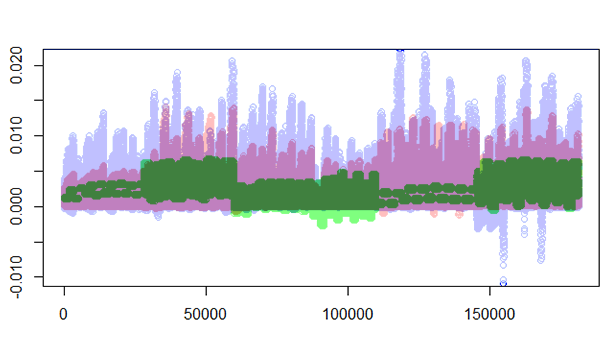
\includegraphics[width = 0.8\textwidth]{mlp}
\caption[Comparison between real data displacements and RF and MLP predictions of the same displacements]{Comparison between real data displacements and RF and MLP predictions of the same displacements. The y axis represents the displacement of the point in the z axis of the Cartesian coordinate system where the breasts are centred, the x axis represents all the points of the dataset, considering all the 288 patients. The real data displacements are displayed as blue and the displacements predicted by RF and MLP algorithms are respectively displayed as pink and green.}
\label{fig:mlp_res}
\end{figure}

As represented in Figure \ref{fig:mlp_res}, there are 6 distinct blocks regarding the predictions of the displacement in z corresponding to the 6 initial patients to generate the dataset. This leads to the conclusion that MLP mostly relies on the breasts shape in not some much in all the other additional features. Another attempt that could be done in order to improve the results generated by MLP, is to assign weights to each input feature, forcing the model to overlook the shape of the model and give more importance to the other features.

Given the unsatisfactory results of MLP, the following experiments will be using a more promising algorithm such as Multi-output regression (MOR) algorithms. This type of algorithms usually lead to better results than RF and allow to predict several target variables in the same model, unlike what was being done so far that for each axis, a different RF model was used. MOR requires the correlation between the target variable that the models tries to predict. Figure \ref{fig:labels_corr} describes the the real values of the target variables that the model may try to predict for all the patients on the dataset.

\begin{figure}[!htb]
\centering
\scalebox{1.0}{%
\begin{tabular}{cc}
\subfloat[Displacement on x axis]{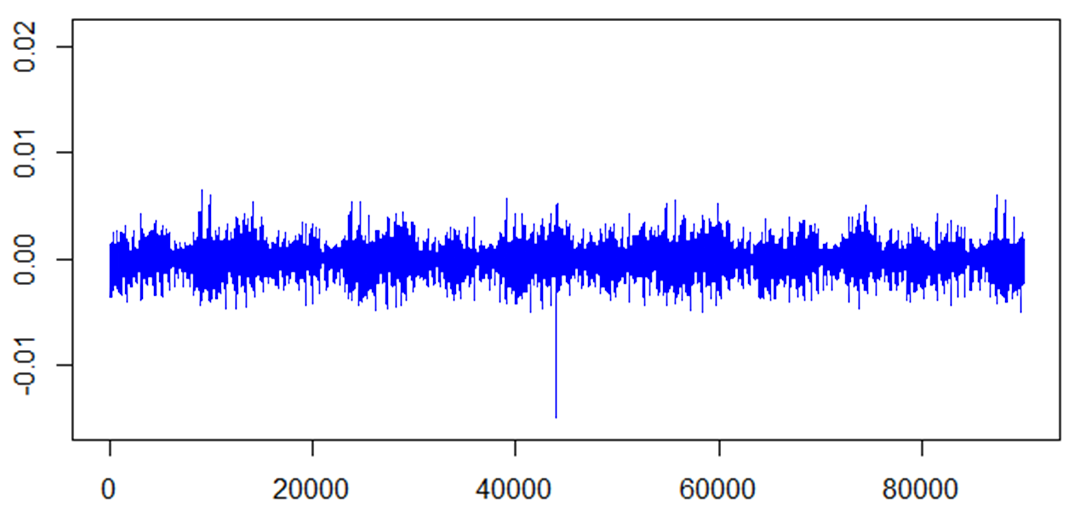
\includegraphics[width = 3.2in]{disp_x}\label{fig:prone}} &
\subfloat[Displacement on y axis]{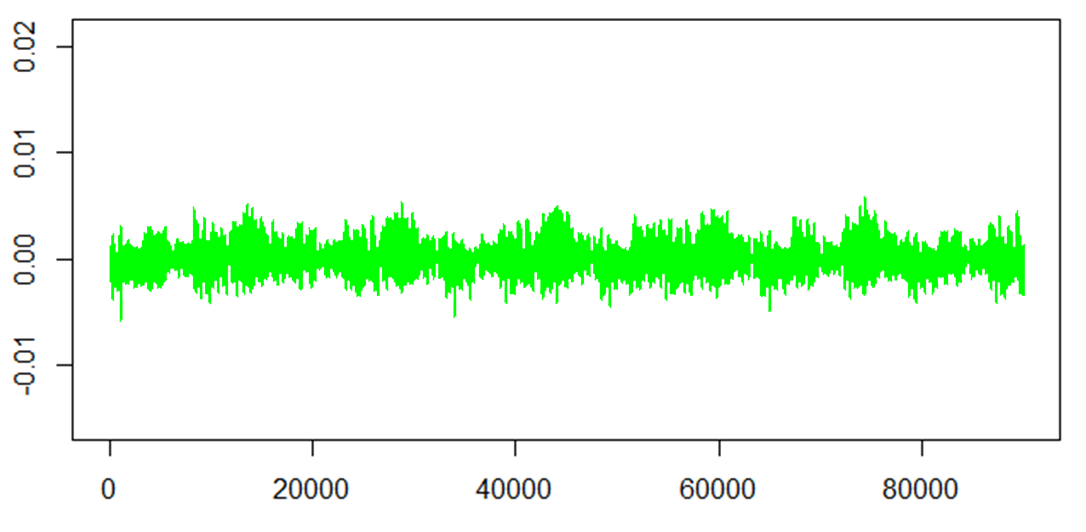
\includegraphics[width = 3.2in]{disp_y}\label{fig:prone_l}}\\
\subfloat[Displacement on z axis]{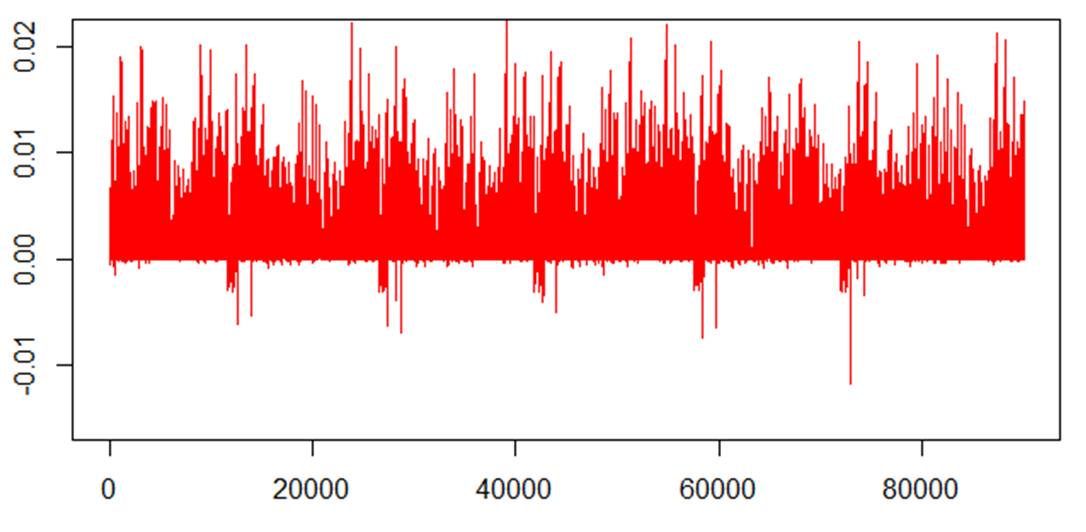
\includegraphics[width = 3.2in]{disp_z}\label{fig:supine}} &
\subfloat[Comparison between the displacements on the three axis]{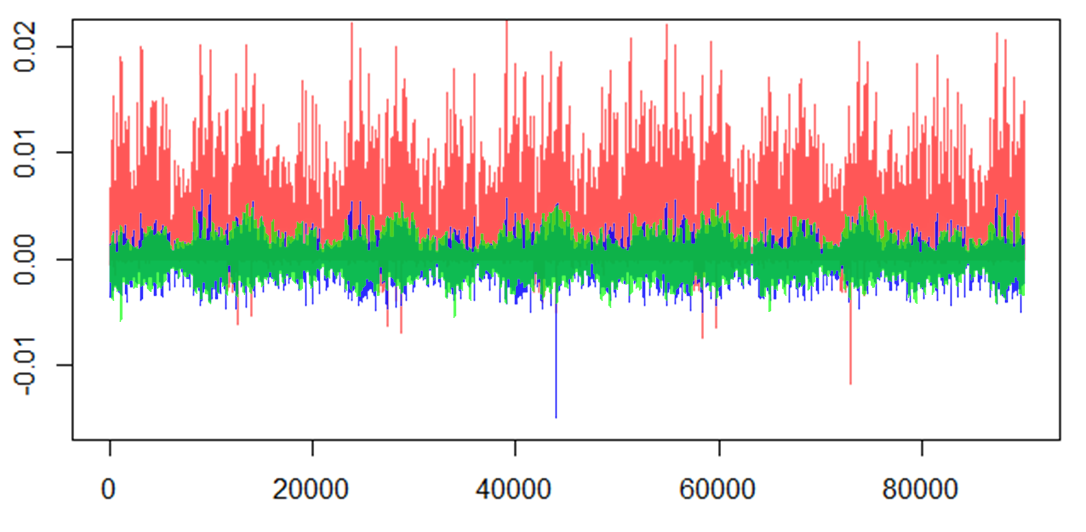
\includegraphics[width = 3.2in]{all_disp_opac}\label{fig:supine_l}}
\end{tabular}
}
\caption[Displacement between the pos and pre-surgical 3D models for all the points of the patients in the dataset]{Displacement between the pos and pre-surgical 3D models for all the points of the patients in the dataset. The y values represent the displacement in meters of each point of each patient, represented in x. Being equally order we can assume that the same value on x in any image represents the same point on the dataset.}
\label{fig:labels_corr}
\end{figure}

By analysing the Figure \ref{fig:labels_corr} and the values of the displacements on the different axis, and knowing that the same value of x on any figure, represents the same point of the dataset and consequently the same patient with the same properties, the displacement on x and y axis seems widely correlated. The correlation between the z displacement and the other two labels, may be correlated but with a lower degree of correlation.

In order to obtain the prediction results for MOR models, two more scenarios were created using the same features as in scenarios 8 and 12. Scenario 13 consists on using the features to predict the displacement on x, y and z axis. Scenario 14 is based on predicting the displacement on x and y axis using MOR and the displacement of z axis using RF. Both the global and local evaluation metrics for these scenarios may be found in Tables \ref{tab:scen13_g}, \ref{tab:scen13_l}, \ref{tab:scen14_g} and \ref{tab:scen14_l}.

\begin{table}[!htb]
\centering
\begin{tabular}{lll|l|l|l|l|l|l|}
\cline{4-9}
                                          &                                                                                                    &                                                              & \begin{tabular}[c]{@{}l@{}}predicted\\  to POS\end{tabular} & \begin{tabular}[c]{@{}l@{}}POS to \\ predicted\end{tabular} & pre to pos & pos to pre & \begin{tabular}[c]{@{}l@{}}predicted\\  to pre\end{tabular} & \begin{tabular}[c]{@{}l@{}}pre to \\ predicted\end{tabular} \\ \hline
\multicolumn{1}{|l|}{\multirow{3}{*}{3D}} & \multicolumn{1}{l|}{\multirow{2}{*}{\begin{tabular}[c]{@{}l@{}}Euclidean\\ Distance\end{tabular}}} & Mean                                                         & 1,227                                                       & 1,225                                                       & 1,758      & 1,731      & 1,934                                                       & 1,950                                                       \\ \cline{3-9} 
\multicolumn{1}{|l|}{}                    & \multicolumn{1}{l|}{}                                                                              & \begin{tabular}[c]{@{}l@{}}Standard\\ Deviation\end{tabular} & 0,863                                                       & 0,857                                                       & 1,333      & 1,277      & 1,194                                                       & 1,226                                                       \\ \cline{2-9} 
\multicolumn{1}{|l|}{}                    & \multicolumn{1}{l|}{\begin{tabular}[c]{@{}l@{}}Hausdorff\\ Distance\end{tabular}}                  &                                                              & 4,336                                                       & 5,280                                                       & 6,513      & 6,317      & 5,382                                                       & 5,555                                                       \\ \hline
\multicolumn{1}{|l|}{\multirow{3}{*}{1D}} & \multicolumn{1}{l|}{\multirow{2}{*}{\begin{tabular}[c]{@{}l@{}}Euclidean\\ Distance\end{tabular}}} & Mean                                                         & 0,114                                                       & 0,114                                                       & 0,160      & 0,110      & 0,127                                                       & 0,173                                                       \\ \cline{3-9} 
\multicolumn{1}{|l|}{}                    & \multicolumn{1}{l|}{}                                                                              & \begin{tabular}[c]{@{}l@{}}Standard\\ Deviation\end{tabular} & 0,121                                                       & 0,128                                                       & 0,346      & 0,110      & 0,121                                                       & 0,355                                                       \\ \cline{2-9} 
\multicolumn{1}{|l|}{}                    & \multicolumn{1}{l|}{\begin{tabular}[c]{@{}l@{}}Hausdorff\\ Distance\end{tabular}}                  &                                                              & 0,939                                                       & 1,096                                                       & 3,168      & 0,704      & 0,747                                                       & 3,403                                                       \\ \hline
\end{tabular}
\caption{Global Evaluation Metrics for Scenario 13}
\label{tab:scen13_g}
\end{table} 

\begin{table}[!htb]
\centering
\begin{tabular}{lll|l|l|l|}
\cline{4-6}
                                          &                                                                                                    &                                                              & \begin{tabular}[c]{@{}l@{}}predicted\\  to POS\end{tabular} & pre to pos & \begin{tabular}[c]{@{}l@{}}predicted\\  to pre\end{tabular} \\ \hline
\multicolumn{1}{|l|}{\multirow{3}{*}{3D}} & \multicolumn{1}{l|}{\multirow{2}{*}{\begin{tabular}[c]{@{}l@{}}Euclidean\\ Distance\end{tabular}}} & Mean                                                         & 1,298                                                       & 2,206      & 2,224                                                       \\ \cline{3-6} 
\multicolumn{1}{|l|}{}                    & \multicolumn{1}{l|}{}                                                                              & \begin{tabular}[c]{@{}l@{}}Standard\\ Deviation\end{tabular} & 0,983                                                       & 1,920      & 1,523                                                       \\ \cline{2-6} 
\multicolumn{1}{|l|}{}                    & \multicolumn{1}{l|}{\begin{tabular}[c]{@{}l@{}}Hausdorff\\ Distance\end{tabular}}                  &                                                              & 4,857                                                       & 8,410      & 6,115                                                       \\ \hline
\multicolumn{1}{|l|}{\multirow{3}{*}{1D}} & \multicolumn{1}{l|}{\multirow{2}{*}{\begin{tabular}[c]{@{}l@{}}Euclidean\\ Distance\end{tabular}}} & Mean                                                         & 1,000                                                       & 1,904      & 2,062                                                       \\ \cline{3-6} 
\multicolumn{1}{|l|}{}                    & \multicolumn{1}{l|}{}                                                                              & \begin{tabular}[c]{@{}l@{}}Standard\\ Deviation\end{tabular} & 0,968                                                       & 1,929      & 1,563                                                       \\ \cline{2-6} 
\multicolumn{1}{|l|}{}                    & \multicolumn{1}{l|}{\begin{tabular}[c]{@{}l@{}}Hausdorff\\ Distance\end{tabular}}                  &                                                              & 4,498                                                       & 8,092      & 5,999                                                       \\ \hline
\end{tabular}
\caption{Local Evaluation Metrics for Scenario 13}
\label{tab:scen13_l}
\end{table}

\begin{table}[!htb]
\centering
\begin{tabular}{lll|l|l|l|l|l|l|}
\cline{4-9}
                                          &                                                                                                    &                                                              & \begin{tabular}[c]{@{}l@{}}predicted\\  to POS\end{tabular} & \begin{tabular}[c]{@{}l@{}}POS to \\ predicted\end{tabular} & pre to pos & pos to pre & \begin{tabular}[c]{@{}l@{}}predicted\\  to pre\end{tabular} & \begin{tabular}[c]{@{}l@{}}pre to \\ predicted\end{tabular} \\ \hline
\multicolumn{1}{|l|}{\multirow{3}{*}{3D}} & \multicolumn{1}{l|}{\multirow{2}{*}{\begin{tabular}[c]{@{}l@{}}Euclidean\\ Distance\end{tabular}}} & Mean                                                         & 1,175                                                       & 1,173                                                       & 1,758      & 1,731      & 1,883                                                       & 1,897                                                       \\ \cline{3-9} 
\multicolumn{1}{|l|}{}                    & \multicolumn{1}{l|}{}                                                                              & \begin{tabular}[c]{@{}l@{}}Standard\\ Deviation\end{tabular} & 0,851                                                       & 0,844                                                       & 1,333      & 1,277      & 1,181                                                       & 1,208                                                       \\ \cline{2-9} 
\multicolumn{1}{|l|}{}                    & \multicolumn{1}{l|}{\begin{tabular}[c]{@{}l@{}}Hausdorff\\ Distance\end{tabular}}                  &                                                              & 4,277                                                       & 4,214                                                       & 6,513      & 6,317      & 5,246                                                       & 5,418                                                       \\ \hline
\multicolumn{1}{|l|}{\multirow{3}{*}{1D}} & \multicolumn{1}{l|}{\multirow{2}{*}{\begin{tabular}[c]{@{}l@{}}Euclidean\\ Distance\end{tabular}}} & Mean                                                         & 0,106                                                       & 0,105                                                       & 0,160      & 0,110      & 0,120                                                       & 0,162                                                       \\ \cline{3-9} 
\multicolumn{1}{|l|}{}                    & \multicolumn{1}{l|}{}                                                                              & \begin{tabular}[c]{@{}l@{}}Standard\\ Deviation\end{tabular} & 0,117                                                       & 0,118                                                       & 0,346      & 0,110      & 0,116                                                       & 0,330                                                       \\ \cline{2-9} 
\multicolumn{1}{|l|}{}                    & \multicolumn{1}{l|}{\begin{tabular}[c]{@{}l@{}}Hausdorff\\ Distance\end{tabular}}                  &                                                              & 0,953                                                       & 0,964                                                       & 3,168      & 0,704      & 0,711                                                       & 3,166                                                       \\ \hline
\end{tabular}
\caption{Global Evaluation Metrics for Scenario 14}
\label{tab:scen14_g}
\end{table}

\begin{table}[!htb]
\centering
\begin{tabular}{lll|l|l|l|}
\cline{4-6}
                                          &                                                                                                    &                                                              & \begin{tabular}[c]{@{}l@{}}predicted\\  to POS\end{tabular} & pre to pos & \begin{tabular}[c]{@{}l@{}}predicted\\  to pre\end{tabular} \\ \hline
\multicolumn{1}{|l|}{\multirow{3}{*}{3D}} & \multicolumn{1}{l|}{\multirow{2}{*}{\begin{tabular}[c]{@{}l@{}}Euclidean\\ Distance\end{tabular}}} & Mean                                                         & 1,241                                                       & 2,206      & 2,186                                                       \\ \cline{3-6} 
\multicolumn{1}{|l|}{}                    & \multicolumn{1}{l|}{}                                                                              & \begin{tabular}[c]{@{}l@{}}Standard\\ Deviation\end{tabular} & 0,966                                                       & 1,920      & 1,518                                                       \\ \cline{2-6} 
\multicolumn{1}{|l|}{}                    & \multicolumn{1}{l|}{\begin{tabular}[c]{@{}l@{}}Hausdorff\\ Distance\end{tabular}}                  &                                                              & 4,767                                                       & 8,410      & 5,938                                                       \\ \hline
\multicolumn{1}{|l|}{\multirow{3}{*}{1D}} & \multicolumn{1}{l|}{\multirow{2}{*}{\begin{tabular}[c]{@{}l@{}}Euclidean\\ Distance\end{tabular}}} & Mean                                                         & 0,924                                                       & 1,904      & 1,981                                                       \\ \cline{3-6} 
\multicolumn{1}{|l|}{}                    & \multicolumn{1}{l|}{}                                                                              & \begin{tabular}[c]{@{}l@{}}Standard\\ Deviation\end{tabular} & 0,942                                                       & 1,929      & 1,565                                                       \\ \cline{2-6} 
\multicolumn{1}{|l|}{}                    & \multicolumn{1}{l|}{\begin{tabular}[c]{@{}l@{}}Hausdorff\\ Distance\end{tabular}}                  &                                                              & 4,369                                                       & 8,092      & 5,830                                                       \\ \hline
\end{tabular}
\caption{Local Evaluation Metrics for Scenario 14}
\label{tab:scen14_l}
\end{table}


From the results described in Tables \ref{tab:scen13_g}, \ref{tab:scen13_l}, \ref{tab:scen14_g} and \ref{tab:scen14_l}, the fact of scenario 14 outperforms scenario 13 proves the lack of correlation between the z displacement and both the x displacement and y displacement. By comparing scenario 14, and despite of the good results, with the RF implementations on scenarios 8 and 12, a slight decrease of the evaluation metrics result is visible. Some parametrization tuning of MOR should be analysed in more detail.

The scenarios presented so far only counted with 3D models of the surface of patients' breasts. Using additional points such as internal points of the breasts' 3D models, may aid the prediction of deformation. In order to study this possibility, a few more scenarios were analysed. In spite of the use of internal points, those were only used in order to train the model. As soon as it was trained, it was applied to the same test set as in all of the other scenarios. The test set only contains points regrading the breast's surface.

\begin{table}[!htb]
\centering
\begin{tabular}{lll|l|l|l|l|l|l|}
\cline{4-9}
                                          &                                                                                                    &                                                              & \begin{tabular}[c]{@{}l@{}}predicted\\  to POS\end{tabular} & \begin{tabular}[c]{@{}l@{}}POS to \\ predicted\end{tabular} & pre to pos & pos to pre & \begin{tabular}[c]{@{}l@{}}predicted\\  to pre\end{tabular} & \begin{tabular}[c]{@{}l@{}}pre to \\ predicted\end{tabular} \\ \hline
\multicolumn{1}{|l|}{\multirow{3}{*}{3D}} & \multicolumn{1}{l|}{\multirow{2}{*}{\begin{tabular}[c]{@{}l@{}}Euclidean\\ Distance\end{tabular}}} & Mean                                                         & 1.044                                                       & 1.043                                                       & 1.555      & 1.529      & 1.652                                                       & 1.670                                                       \\ \cline{3-9} 
\multicolumn{1}{|l|}{}                    & \multicolumn{1}{l|}{}                                                                              & \begin{tabular}[c]{@{}l@{}}Standard\\ Deviation\end{tabular} & 0.840                                                       & 0.837                                                       & 1.382      & 1.319      & 1.257                                                       & 1.296                                                       \\ \cline{2-9} 
\multicolumn{1}{|l|}{}                    & \multicolumn{1}{l|}{\begin{tabular}[c]{@{}l@{}}Hausdorff\\ Distance\end{tabular}}                  &                                                              & 4.875                                                       & 4.817                                                       & 7.107      & 6.406      & 5.533                                                       & 5.923                                                       \\ \hline
\multicolumn{1}{|l|}{\multirow{3}{*}{1D}} & \multicolumn{1}{l|}{\multirow{2}{*}{\begin{tabular}[c]{@{}l@{}}Euclidean\\ Distance\end{tabular}}} & Mean                                                         & 0.055                                                       & 0.055                                                       & 0.080      & 0.055      & 0.060                                                       & 0.083                                                       \\ \cline{3-9} 
\multicolumn{1}{|l|}{}                    & \multicolumn{1}{l|}{}                                                                              & \begin{tabular}[c]{@{}l@{}}Standard\\ Deviation\end{tabular} & 0.063                                                       & 0.068                                                       & 0.236      & 0.060      & 0.062                                                       & 0.238                                                       \\ \cline{2-9} 
\multicolumn{1}{|l|}{}                    & \multicolumn{1}{l|}{\begin{tabular}[c]{@{}l@{}}Hausdorff\\ Distance\end{tabular}}                  &                                                              & 0.659                                                       & 0.789                                                       & 3.154      & 0.477      & 0.465                                                       & 3.287                                                       \\ \hline
\end{tabular}
\caption{Global Evaluation Metrics for Scenario 15}
\label{tab:scen15_g}
\end{table}

\begin{table}[!htb]
\centering
\begin{tabular}{lll|l|l|l|}
\cline{4-6}
                                          &                                                                                                    &                                                              & \begin{tabular}[c]{@{}l@{}}predicted\\  to POS\end{tabular} & pre to pos & \begin{tabular}[c]{@{}l@{}}predicted\\  to pre\end{tabular} \\ \hline
\multicolumn{1}{|l|}{\multirow{3}{*}{3D}} & \multicolumn{1}{l|}{\multirow{2}{*}{\begin{tabular}[c]{@{}l@{}}Euclidean\\ Distance\end{tabular}}} & Mean                                                         & 1.077                                                       & 1.919      & 1.912                                                       \\ \cline{3-6} 
\multicolumn{1}{|l|}{}                    & \multicolumn{1}{l|}{}                                                                              & \begin{tabular}[c]{@{}l@{}}Standard\\ Deviation\end{tabular} & 0.911                                                       & 1.940      & 1.611                                                       \\ \cline{2-6} 
\multicolumn{1}{|l|}{}                    & \multicolumn{1}{l|}{\begin{tabular}[c]{@{}l@{}}Hausdorff\\ Distance\end{tabular}}                  &                                                              & 5.352                                                       & 9.510      & 6.620                                                       \\ \hline
\multicolumn{1}{|l|}{\multirow{3}{*}{1D}} & \multicolumn{1}{l|}{\multirow{2}{*}{\begin{tabular}[c]{@{}l@{}}Euclidean\\ Distance\end{tabular}}} & Mean                                                         & 0.817                                                       & 1.693      & 1.759                                                       \\ \cline{3-6} 
\multicolumn{1}{|l|}{}                    & \multicolumn{1}{l|}{}                                                                              & \begin{tabular}[c]{@{}l@{}}Standard\\ Deviation\end{tabular} & 0.889                                                       & 1.908      & 1.620                                                       \\ \cline{2-6} 
\multicolumn{1}{|l|}{}                    & \multicolumn{1}{l|}{\begin{tabular}[c]{@{}l@{}}Hausdorff\\ Distance\end{tabular}}                  &                                                              & 5.003                                                       & 9.147      & 6.475                                                       \\ \hline
\end{tabular}
\caption{Local Evaluation Metrics for Scenario 15}
\label{tab:scen15_l}
\end{table}

\begin{table}[!htb]
\centering
\begin{tabular}{lll|l|l|l|l|l|l|}
\cline{4-9}
                                          &                                                                                                    &                                                              & \begin{tabular}[c]{@{}l@{}}predicted\\  to POS\end{tabular} & \begin{tabular}[c]{@{}l@{}}POS to \\ predicted\end{tabular} & pre to pos & pos to pre & \begin{tabular}[c]{@{}l@{}}predicted\\  to pre\end{tabular} & \begin{tabular}[c]{@{}l@{}}pre to \\ predicted\end{tabular} \\ \hline
\multicolumn{1}{|l|}{\multirow{3}{*}{3D}} & \multicolumn{1}{l|}{\multirow{2}{*}{\begin{tabular}[c]{@{}l@{}}Euclidean\\ Distance\end{tabular}}} & Mean                                                         & 1.143                                                       & 1.142                                                       & 1.555      & 1.529      & 1.779                                                       & 1.798                                                       \\ \cline{3-9} 
\multicolumn{1}{|l|}{}                    & \multicolumn{1}{l|}{}                                                                              & \begin{tabular}[c]{@{}l@{}}Standard\\ Deviation\end{tabular} & 0.874                                                       & 0.870                                                       & 1.382      & 1.319      & 1.286                                                       & 1.327                                                       \\ \cline{2-9} 
\multicolumn{1}{|l|}{}                    & \multicolumn{1}{l|}{\begin{tabular}[c]{@{}l@{}}Hausdorff\\ Distance\end{tabular}}                  &                                                              & 4.997                                                       & 4.924                                                       & 7.107      & 6.406      & 5.706                                                       & 4.924                                                       \\ \hline
\multicolumn{1}{|l|}{\multirow{3}{*}{1D}} & \multicolumn{1}{l|}{\multirow{2}{*}{\begin{tabular}[c]{@{}l@{}}Euclidean\\ Distance\end{tabular}}} & Mean                                                         & 0.0599                                                      & 0.0609                                                      & 0.080      & 0.0553     & 0.0639                                                      & 0.0917                                                      \\ \cline{3-9} 
\multicolumn{1}{|l|}{}                    & \multicolumn{1}{l|}{}                                                                              & \begin{tabular}[c]{@{}l@{}}Standard\\ Deviation\end{tabular} & 0.0667                                                      & 0.0806                                                      & 0.236      & 0.0604     & 0.0668                                                      & 0.2744                                                      \\ \cline{2-9} 
\multicolumn{1}{|l|}{}                    & \multicolumn{1}{l|}{\begin{tabular}[c]{@{}l@{}}Hausdorff\\ Distance\end{tabular}}                  &                                                              & 0.626                                                       & 1.0595                                                      & 3.155      & 0.4767     & 0.4941                                                      & 3.7512                                                      \\ \hline
\end{tabular}
\caption{Global Evaluation Metrics for Scenario 16}
\label{tab:scen16_g}
\end{table}

\begin{table}[!htb]
\centering
\begin{tabular}{lll|l|l|l|}
\cline{4-6}
                                          &                                                                                                    &                                                              & \begin{tabular}[c]{@{}l@{}}predicted\\  to POS\end{tabular} & pre to pos & \begin{tabular}[c]{@{}l@{}}predicted\\  to pre\end{tabular} \\ \hline
\multicolumn{1}{|l|}{\multirow{3}{*}{3D}} & \multicolumn{1}{l|}{\multirow{2}{*}{\begin{tabular}[c]{@{}l@{}}Euclidean\\ Distance\end{tabular}}} & Mean                                                         & 1.182                                                       & 1.919      & 2.029                                                       \\ \cline{3-6} 
\multicolumn{1}{|l|}{}                    & \multicolumn{1}{l|}{}                                                                              & \begin{tabular}[c]{@{}l@{}}Standard\\ Deviation\end{tabular} & 0.953                                                       & 1.940      & 1.624                                                       \\ \cline{2-6} 
\multicolumn{1}{|l|}{}                    & \multicolumn{1}{l|}{\begin{tabular}[c]{@{}l@{}}Hausdorff\\ Distance\end{tabular}}                  &                                                              & 5.492                                                       & 9.510      & 6.694                                                       \\ \hline
\multicolumn{1}{|l|}{\multirow{3}{*}{1D}} & \multicolumn{1}{l|}{\multirow{2}{*}{\begin{tabular}[c]{@{}l@{}}Euclidean\\ Distance\end{tabular}}} & Mean                                                         & 0.933                                                       & 1.693      & 1.905                                                       \\ \cline{3-6} 
\multicolumn{1}{|l|}{}                    & \multicolumn{1}{l|}{}                                                                              & \begin{tabular}[c]{@{}l@{}}Standard\\ Deviation\end{tabular} & 0.930                                                       & 1.908      & 1.629                                                       \\ \cline{2-6} 
\multicolumn{1}{|l|}{}                    & \multicolumn{1}{l|}{\begin{tabular}[c]{@{}l@{}}Hausdorff\\ Distance\end{tabular}}                  &                                                              & 5.134                                                       & 9.147      & 6.544                                                       \\ \hline
\end{tabular}
\caption{Local Evaluation Metrics for Scenario 16}
\label{tab:scen16_l}
\end{table}

\begin{table}[!htb]
\centering
\begin{tabular}{lll|l|l|l|l|l|l|}
\cline{4-9}
                                          &                                                                                                    &                                                              & \begin{tabular}[c]{@{}l@{}}predicted\\  to POS\end{tabular} & \begin{tabular}[c]{@{}l@{}}POS to \\ predicted\end{tabular} & pre to pos & pos to pre & \begin{tabular}[c]{@{}l@{}}predicted\\  to pre\end{tabular} & \begin{tabular}[c]{@{}l@{}}pre to \\ predicted\end{tabular} \\ \hline
\multicolumn{1}{|l|}{\multirow{3}{*}{3D}} & \multicolumn{1}{l|}{\multirow{2}{*}{\begin{tabular}[c]{@{}l@{}}Euclidean\\ Distance\end{tabular}}} & Mean                                                         & 1.071                                                       & 1.069                                                       & 1.555      & 1.529      & 1.689                                                       & 1.705                                                       \\ \cline{3-9} 
\multicolumn{1}{|l|}{}                    & \multicolumn{1}{l|}{}                                                                              & \begin{tabular}[c]{@{}l@{}}Standard\\ Deviation\end{tabular} & 0.846                                                       & 0.841                                                       & 1.382      & 1.319      & 1.251                                                       & 1.287                                                       \\ \cline{2-9} 
\multicolumn{1}{|l|}{}                    & \multicolumn{1}{l|}{\begin{tabular}[c]{@{}l@{}}Hausdorff\\ Distance\end{tabular}}                  &                                                              & 4.941                                                       & 4.846                                                       & 7.107      & 6.406      & 5.465                                                       & 5.835                                                       \\ \hline
\multicolumn{1}{|l|}{\multirow{3}{*}{1D}} & \multicolumn{1}{l|}{\multirow{2}{*}{\begin{tabular}[c]{@{}l@{}}Euclidean\\ Distance\end{tabular}}} & Mean                                                         & 0.055                                                       & 0.056                                                       & 0.080      & 0.055      & 0.060                                                       & 0.083                                                       \\ \cline{3-9} 
\multicolumn{1}{|l|}{}                    & \multicolumn{1}{l|}{}                                                                              & \begin{tabular}[c]{@{}l@{}}Standard\\ Deviation\end{tabular} & 0.063                                                       & 0.068                                                       & 0.236      & 0.060      & 0.062                                                       & 0.239                                                       \\ \cline{2-9} 
\multicolumn{1}{|l|}{}                    & \multicolumn{1}{l|}{\begin{tabular}[c]{@{}l@{}}Hausdorff\\ Distance\end{tabular}}                  &                                                              & 0.646                                                       & 0.794                                                       & 3.155      & 0.477      & 0.468                                                       & 3.330                                                       \\ \hline
\end{tabular}
\caption{Global Evaluation Metrics for Scenario 17}
\label{tab:scen17_g}
\end{table}

\begin{table}[!htb]
\centering
\begin{tabular}{lll|l|l|l|}
\cline{4-6}
                                          &                                                                                                    &                                                              & \begin{tabular}[c]{@{}l@{}}predicted\\  to POS\end{tabular} & pre to pos & \begin{tabular}[c]{@{}l@{}}predicted\\  to pre\end{tabular} \\ \hline
\multicolumn{1}{|l|}{\multirow{3}{*}{3D}} & \multicolumn{1}{l|}{\multirow{2}{*}{\begin{tabular}[c]{@{}l@{}}Euclidean\\ Distance\end{tabular}}} & Mean                                                         & 1.105                                                       & 1.919      & 1.936                                                       \\ \cline{3-6} 
\multicolumn{1}{|l|}{}                    & \multicolumn{1}{l|}{}                                                                              & \begin{tabular}[c]{@{}l@{}}Standard\\ Deviation\end{tabular} & 0.920                                                       & 1.940      & 1.584                                                       \\ \cline{2-6} 
\multicolumn{1}{|l|}{}                    & \multicolumn{1}{l|}{\begin{tabular}[c]{@{}l@{}}Hausdorff\\ Distance\end{tabular}}                  &                                                              & 5.439                                                       & 9.510      & 6.441                                                       \\ \hline
\multicolumn{1}{|l|}{\multirow{3}{*}{1D}} & \multicolumn{1}{l|}{\multirow{2}{*}{\begin{tabular}[c]{@{}l@{}}Euclidean\\ Distance\end{tabular}}} & Mean                                                         & 0.828                                                       & 1.693      & 1.763                                                       \\ \cline{3-6} 
\multicolumn{1}{|l|}{}                    & \multicolumn{1}{l|}{}                                                                              & \begin{tabular}[c]{@{}l@{}}Standard\\ Deviation\end{tabular} & 0.898                                                       & 1.908      & 1.598                                                       \\ \cline{2-6} 
\multicolumn{1}{|l|}{}                    & \multicolumn{1}{l|}{\begin{tabular}[c]{@{}l@{}}Hausdorff\\ Distance\end{tabular}}                  &                                                              & 5.076                                                       & 9.147      & 6.284                                                       \\ \hline
\end{tabular}
\caption{Local Evaluation Metrics for Scenario 17}
\label{tab:scen17_l}
\end{table}

The same effect that occurred in scenarios 13 and 14, also occurred as expected on scenarios 16 and 17 as seen in Tables \ref{tab:scen16_g}, \ref{tab:scen16_l}, \ref{tab:scen17_g} and \ref{tab:scen17_l}. As shown in Tables \ref{tab:scen15_g} and \ref{tab:scen15_l}, Scenario 15 leads to the best prediction results.

As previously stated, all the presented scenarios were computed using a LOO strategy. A different train/test split was done as described in section \ref{subsec:labels} were the cases in the dataset were randomly split into train and test sets. Since all the cases in the dataset were generated from 6 initial patients, there is a great probability of a case in the test set having a very similar cases on the training set. This split was done and further tested in order to represent an ideal situation of the breast's deformation prediction. Tables \ref{tab:scen15_g_of}, \ref{tab:scen15_l_of}, \ref{tab:scen17_g_of} and \ref{tab:scen17_l_of} represent global and local evaluation metrics for scenarios 15 and 17 using a random train/test split instead of the LOO strategy.

\begin{table}[!htb]
\centering
\begin{tabular}{lll|l|l|l|l|l|l|}
\cline{4-9}
                                          &                                                                                                    &                                                              & \begin{tabular}[c]{@{}l@{}}predicted\\  to POS\end{tabular} & \begin{tabular}[c]{@{}l@{}}POS to \\ predicted\end{tabular} & pre to pos & pos to pre & \begin{tabular}[c]{@{}l@{}}predicted\\  to pre\end{tabular} & \begin{tabular}[c]{@{}l@{}}pre to \\ predicted\end{tabular} \\ \hline
\multicolumn{1}{|l|}{\multirow{3}{*}{3D}} & \multicolumn{1}{l|}{\multirow{2}{*}{\begin{tabular}[c]{@{}l@{}}Euclidean\\ Distance\end{tabular}}} & Mean                                                         & 0.639                                                       & 0.638                                                       & 1.592      & 1.562      & 1.653                                                       & 1.679                                                       \\ \cline{3-9} 
\multicolumn{1}{|l|}{}                    & \multicolumn{1}{l|}{}                                                                              & \begin{tabular}[c]{@{}l@{}}Standard\\ Deviation\end{tabular} & 0.614                                                       & 0.610                                                       & 1.391      & 1.318      & 1.336                                                       & 1.394                                                       \\ \cline{2-9} 
\multicolumn{1}{|l|}{}                    & \multicolumn{1}{l|}{\begin{tabular}[c]{@{}l@{}}Hausdorff\\ Distance\end{tabular}}                  &                                                              & 3.979                                                       & 3.932                                                       & 7.054      & 6.252      & 5.957                                                       & 6.452                                                       \\ \hline
\multicolumn{1}{|l|}{\multirow{3}{*}{1D}} & \multicolumn{1}{l|}{\multirow{2}{*}{\begin{tabular}[c]{@{}l@{}}Euclidean\\ Distance\end{tabular}}} & Mean                                                         & 0.050                                                       & 0.049                                                       & 0.088      & 0.056      & 0.058                                                       & 0.083                                                       \\ \cline{3-9} 
\multicolumn{1}{|l|}{}                    & \multicolumn{1}{l|}{}                                                                              & \begin{tabular}[c]{@{}l@{}}Standard\\ Deviation\end{tabular} & 0.062                                                       & 0.053                                                       & 0.284      & 0.060      & 0.062                                                       & 0.243                                                       \\ \cline{2-9} 
\multicolumn{1}{|l|}{}                    & \multicolumn{1}{l|}{\begin{tabular}[c]{@{}l@{}}Hausdorff\\ Distance\end{tabular}}                  &                                                              & 0.773                                                       & 0.480                                                       & 3.695      & 0.461      & 0.471                                                       & 3.325                                                       \\ \hline
\end{tabular}
\caption{Global Evaluation Metrics for Scenario 15 using random train/test split}
\label{tab:scen15_g_of}
\end{table}

\begin{table}[!htb]
\centering
\begin{tabular}{lll|l|l|l|}
\cline{4-6}
                                          &                                                                                                    &                                                              & \begin{tabular}[c]{@{}l@{}}predicted\\  to POS\end{tabular} & pre to pos & \begin{tabular}[c]{@{}l@{}}predicted\\  to pre\end{tabular} \\ \hline
\multicolumn{1}{|l|}{\multirow{3}{*}{3D}} & \multicolumn{1}{l|}{\multirow{2}{*}{\begin{tabular}[c]{@{}l@{}}Euclidean\\ Distance\end{tabular}}} & Mean                                                         & 0.644                                                       & 2.019      & 2.001                                                       \\ \cline{3-6} 
\multicolumn{1}{|l|}{}                    & \multicolumn{1}{l|}{}                                                                              & \begin{tabular}[c]{@{}l@{}}Standard\\ Deviation\end{tabular} & 0.630                                                       & 2.046      & 1.826                                                       \\ \cline{2-6} 
\multicolumn{1}{|l|}{}                    & \multicolumn{1}{l|}{\begin{tabular}[c]{@{}l@{}}Hausdorff\\ Distance\end{tabular}}                  &                                                              & 4.090                                                       & 9.927      & 7.420                                                       \\ \hline
\multicolumn{1}{|l|}{\multirow{3}{*}{1D}} & \multicolumn{1}{l|}{\multirow{2}{*}{\begin{tabular}[c]{@{}l@{}}Euclidean\\ Distance\end{tabular}}} & Mean                                                         & 0.501                                                       & 1.732      & 1.631                                                       \\ \cline{3-6} 
\multicolumn{1}{|l|}{}                    & \multicolumn{1}{l|}{}                                                                              & \begin{tabular}[c]{@{}l@{}}Standard\\ Deviation\end{tabular} & 0.624                                                       & 1.941      & 1.648                                                       \\ \cline{2-6} 
\multicolumn{1}{|l|}{}                    & \multicolumn{1}{l|}{\begin{tabular}[c]{@{}l@{}}Hausdorff\\ Distance\end{tabular}}                  &                                                              & 3.870                                                       & 9.190      & 6.710                                                       \\ \hline
\end{tabular}
\caption{Local Evaluation Metrics for Scenario 15 using random train/test split}
\label{tab:scen15_l_of}
\end{table}

\begin{table}[!htb]
\centering
\begin{tabular}{lll|l|l|l|l|l|l|}
\cline{4-9}
                                          &                                                                                                    &                                                              & \begin{tabular}[c]{@{}l@{}}predicted\\  to POS\end{tabular} & \begin{tabular}[c]{@{}l@{}}POS to \\ predicted\end{tabular} & pre to pos & pos to pre & \begin{tabular}[c]{@{}l@{}}predicted\\  to pre\end{tabular} & \begin{tabular}[c]{@{}l@{}}pre to \\ predicted\end{tabular} \\ \hline
\multicolumn{1}{|l|}{\multirow{3}{*}{3D}} & \multicolumn{1}{l|}{\multirow{2}{*}{\begin{tabular}[c]{@{}l@{}}Euclidean\\ Distance\end{tabular}}} & Mean                                                         & 0.6224                                                      & 0.6222                                                      & 1.6423     & 1.6213     & 1.6692                                                      & 1.689                                                       \\ \cline{3-9} 
\multicolumn{1}{|l|}{}                    & \multicolumn{1}{l|}{}                                                                              & \begin{tabular}[c]{@{}l@{}}Standard\\ Deviation\end{tabular} & 0.609                                                       & 0.6082                                                      & 1.4732     & 1.4207     & 1.3839                                                      & 1.4307                                                      \\ \cline{2-9} 
\multicolumn{1}{|l|}{}                    & \multicolumn{1}{l|}{\begin{tabular}[c]{@{}l@{}}Hausdorff\\ Distance\end{tabular}}                  &                                                              & 3.8942                                                      & 3.9134                                                      & 7.4057     & 6.7742     & 6.0621                                                      & 6.5342                                                      \\ \hline
\multicolumn{1}{|l|}{\multirow{3}{*}{1D}} & \multicolumn{1}{l|}{\multirow{2}{*}{\begin{tabular}[c]{@{}l@{}}Euclidean\\ Distance\end{tabular}}} & Mean                                                         & 0.0492                                                      & 0.0491                                                      & 0.082      & 0.057      & 0.0586                                                      & 0.0864                                                      \\ \cline{3-9} 
\multicolumn{1}{|l|}{}                    & \multicolumn{1}{l|}{}                                                                              & \begin{tabular}[c]{@{}l@{}}Standard\\ Deviation\end{tabular} & 0.0545                                                      & 0.0589                                                      & 0.2439     & 0.0614     & 0.0621                                                      & 0.2659                                                      \\ \cline{2-9} 
\multicolumn{1}{|l|}{}                    & \multicolumn{1}{l|}{\begin{tabular}[c]{@{}l@{}}Hausdorff\\ Distance\end{tabular}}                  &                                                              & 0.5079                                                      & 0.6503                                                      & 3.3466     & 0.4656     & 0.4686                                                      & 3.5979                                                      \\ \hline
\end{tabular}
\caption{Global Evaluation Metrics for Scenario 17 using random train/test split}
\label{tab:scen17_g_of}
\end{table}

\begin{table}[!htb]
\centering
\begin{tabular}{lll|l|l|l|}
\cline{4-6}
                                          &                                                                                                    &                                                              & \begin{tabular}[c]{@{}l@{}}predicted\\  to POS\end{tabular} & pre to pos & \begin{tabular}[c]{@{}l@{}}predicted\\  to pre\end{tabular} \\ \hline
\multicolumn{1}{|l|}{\multirow{3}{*}{3D}} & \multicolumn{1}{l|}{\multirow{2}{*}{\begin{tabular}[c]{@{}l@{}}Euclidean\\ Distance\end{tabular}}} & Mean                                                         & 0.6256                                                      & 2.0275     & 1.9845                                                      \\ \cline{3-6} 
\multicolumn{1}{|l|}{}                    & \multicolumn{1}{l|}{}                                                                              & \begin{tabular}[c]{@{}l@{}}Standard\\ Deviation\end{tabular} & 0.6183                                                      & 2.0857     & 1.8396                                                      \\ \cline{2-6} 
\multicolumn{1}{|l|}{}                    & \multicolumn{1}{l|}{\begin{tabular}[c]{@{}l@{}}Hausdorff\\ Distance\end{tabular}}                  &                                                              & 4.0684                                                      & 10.1156    & 7.4468                                                      \\ \hline
\multicolumn{1}{|l|}{\multirow{3}{*}{1D}} & \multicolumn{1}{l|}{\multirow{2}{*}{\begin{tabular}[c]{@{}l@{}}Euclidean\\ Distance\end{tabular}}} & Mean                                                         & 0.4829                                                      & 1.801      & 1.824                                                       \\ \cline{3-6} 
\multicolumn{1}{|l|}{}                    & \multicolumn{1}{l|}{}                                                                              & \begin{tabular}[c]{@{}l@{}}Standard\\ Deviation\end{tabular} & 0.5822                                                      & 2.0485     & 1.8251                                                      \\ \cline{2-6} 
\multicolumn{1}{|l|}{}                    & \multicolumn{1}{l|}{\begin{tabular}[c]{@{}l@{}}Hausdorff\\ Distance\end{tabular}}                  &                                                              & 3.8564                                                      & 9.7239     & 7.2277                                                      \\ \hline
\end{tabular}
\caption{Local Evaluation Metrics for Scenario 17 using random train/test split}
\label{tab:scen17_l_of}
\end{table}

Figure \ref{fig:rf_visual} shows a few visual examples of the prediction results obtained in scenario 12.

\begin{figure}[!htb]
\centering
\scalebox{0.6}{%
\begin{tabular}{cc}
\subfloat[]{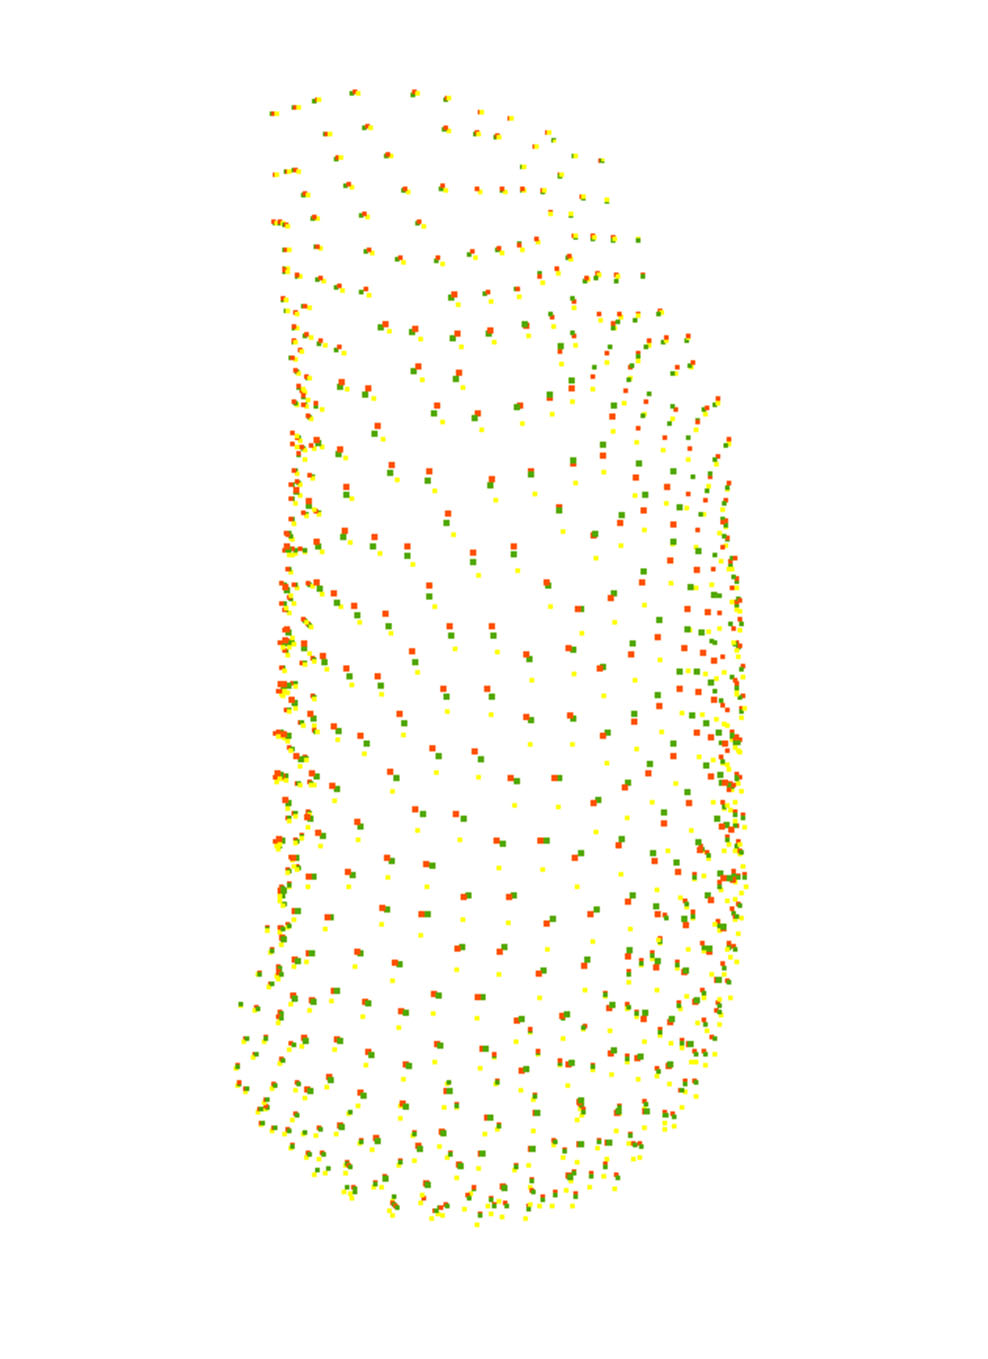
\includegraphics[width = 3in]{visual_pat1}} &
\subfloat[]{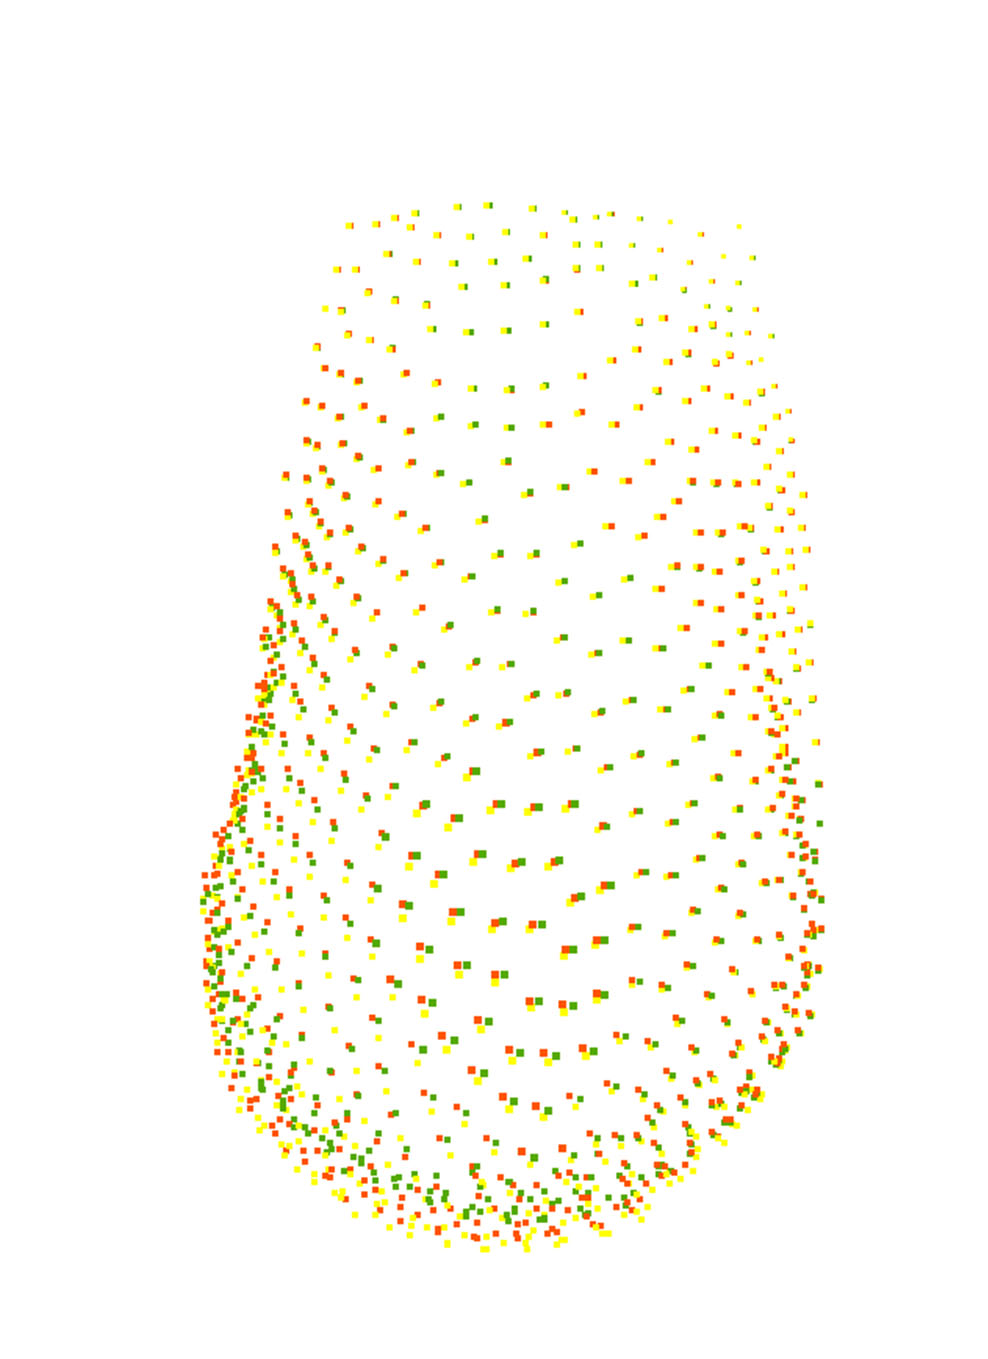
\includegraphics[width = 3in]{visual_pat2}}\\
\subfloat[]{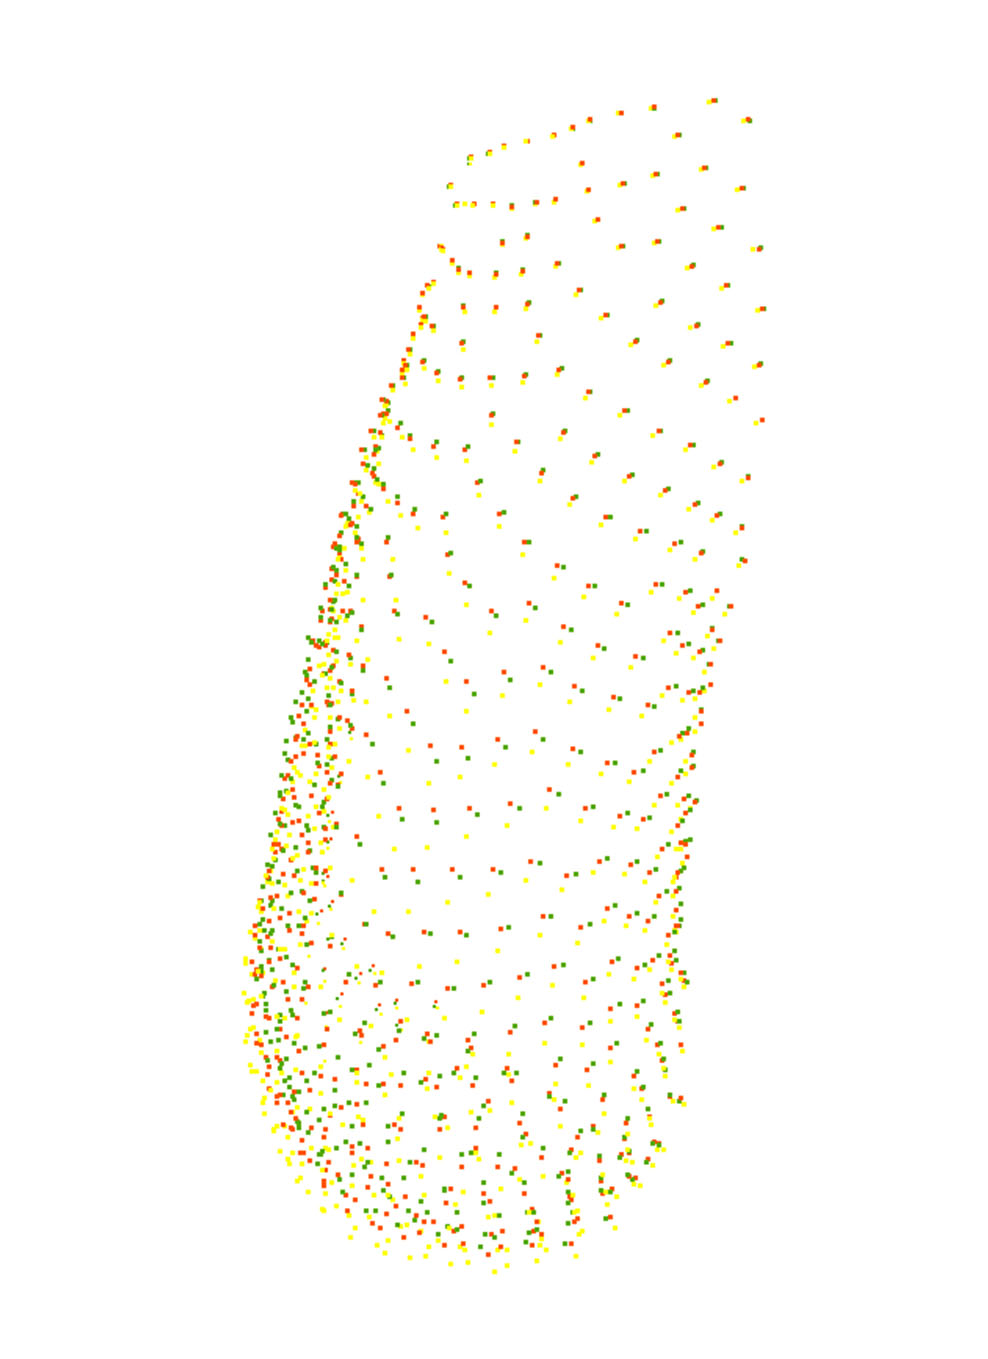
\includegraphics[width = 3in]{visual_pat3}} &
\subfloat[]{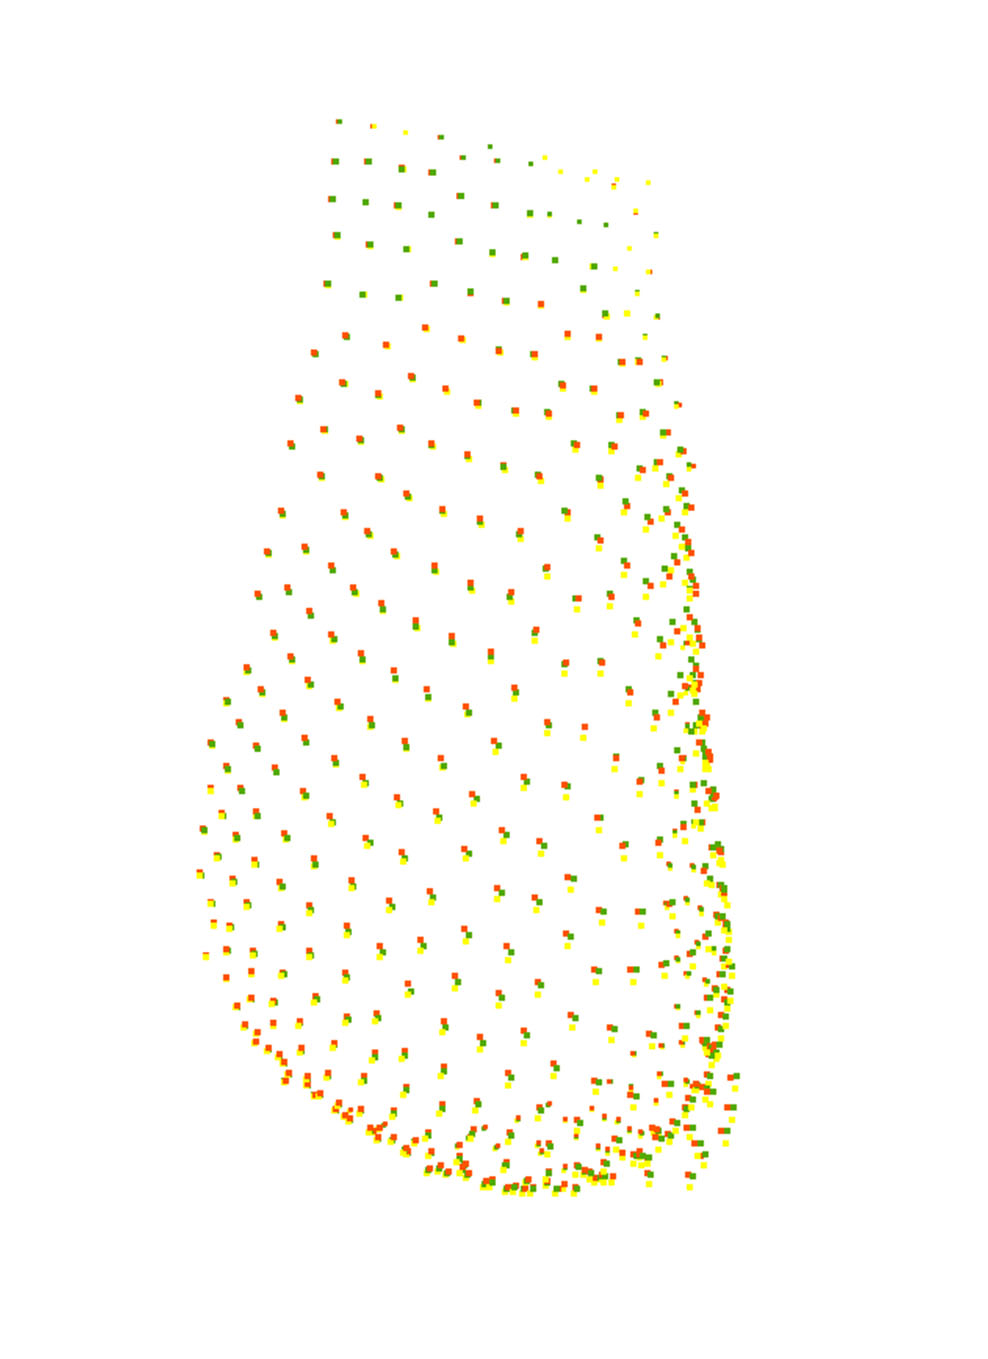
\includegraphics[width = 3in]{visual_pat4}}\\
\subfloat[]{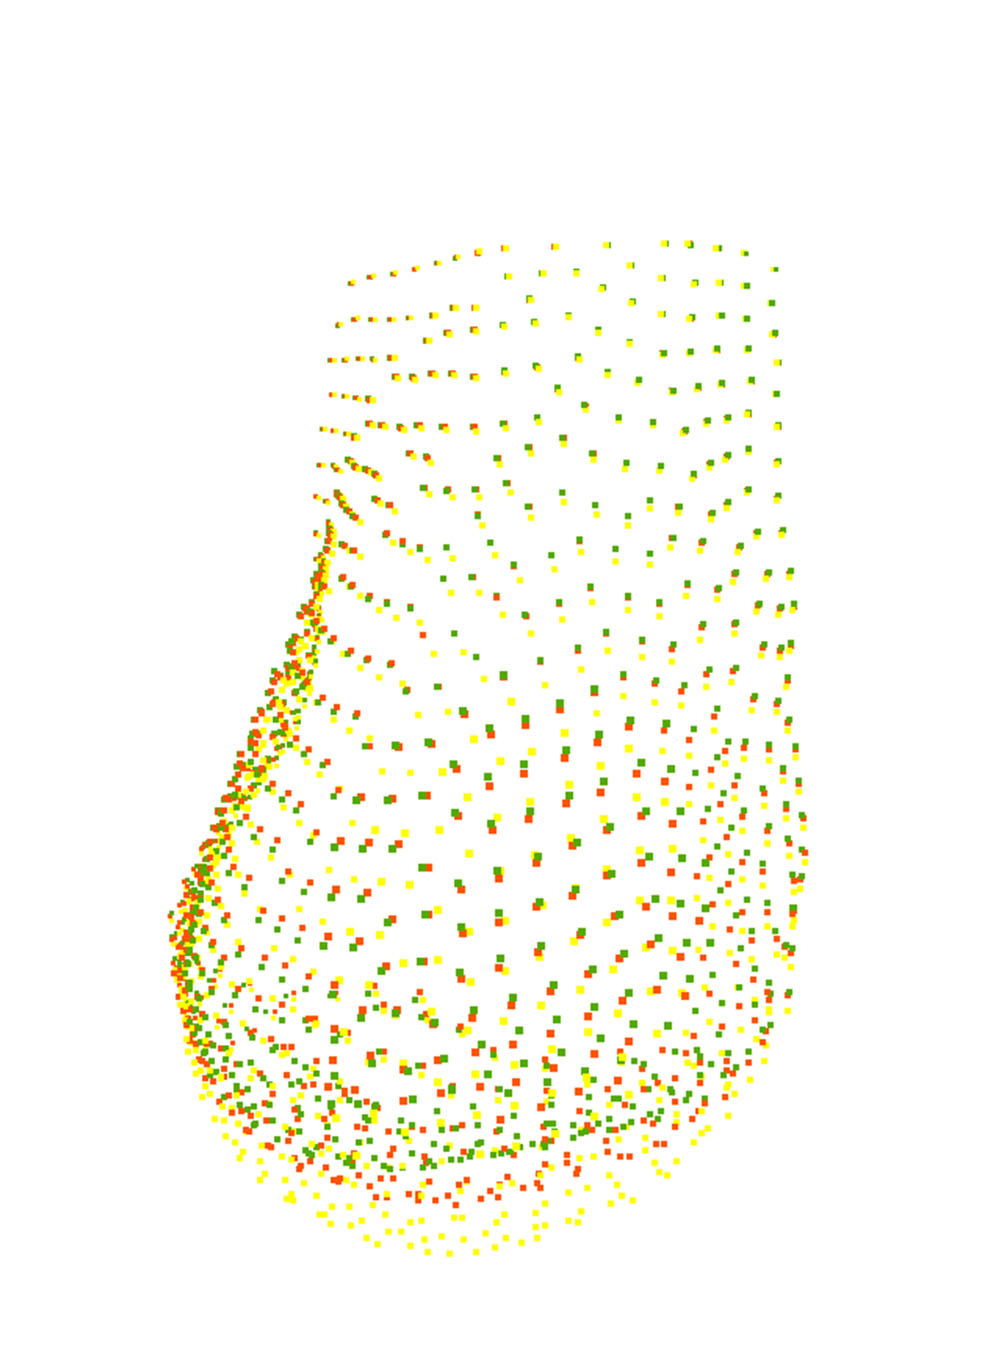
\includegraphics[width = 3in]{visual_pat5}} &
\subfloat[]{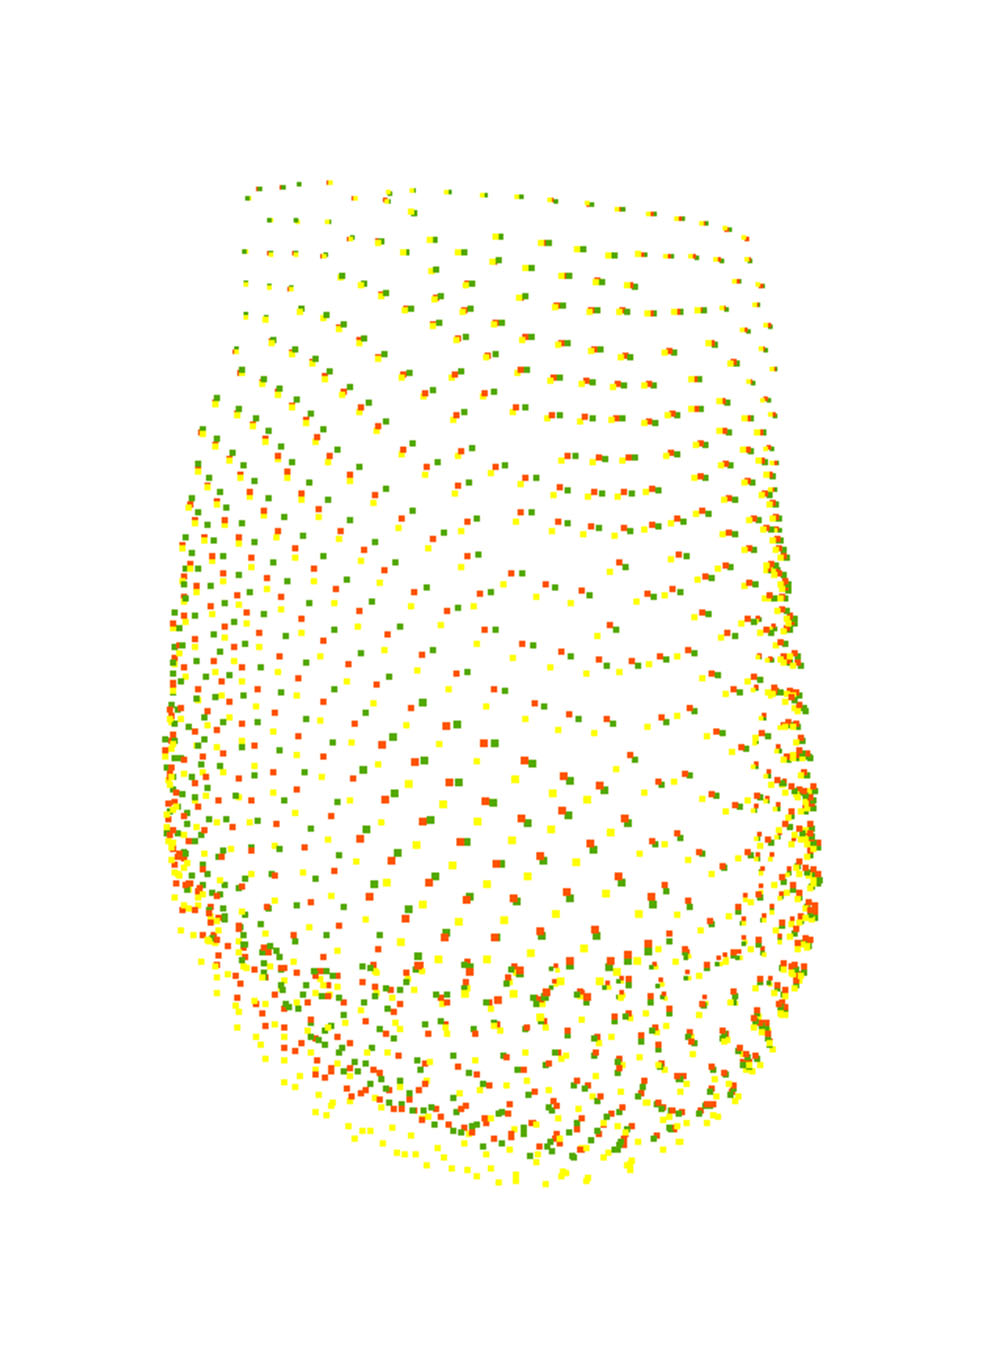
\includegraphics[width = 3in]{visual_pat6}}
\end{tabular}
}
\caption[visual examples of the prediction results obtained in scenario 12]{visual examples of the prediction results obtained in scenario 12}
\label{fig:rf_visual}
\end{figure}

\fi

\section{Predictive errors heatmap} \label{sec:heatmap}

In spite of the good results regarding the mean euclidean distance between the points, the still significant value of the Hausdorff distance points out that some of the points are not moving as much as they should. Analysing the points of the breast were this generally happens would make us understand what parts of the breast's shape are more unreliable. This predictive errors are calculated based on the distance between the predicted point and the correspondent point on the pos-surgical model of the breast. As they can be seen in Figure \ref{fig:heatmap}, the predictive errors are displayed as a heatmap representation in a shape of a breast. The representation of the point in a colour near to red indicates a more inaccurate prediction of the point's displacement.

\begin{figure}[!htb]
\centering
\scalebox{0.6}{%
\begin{tabular}{cc}
\subfloat[]{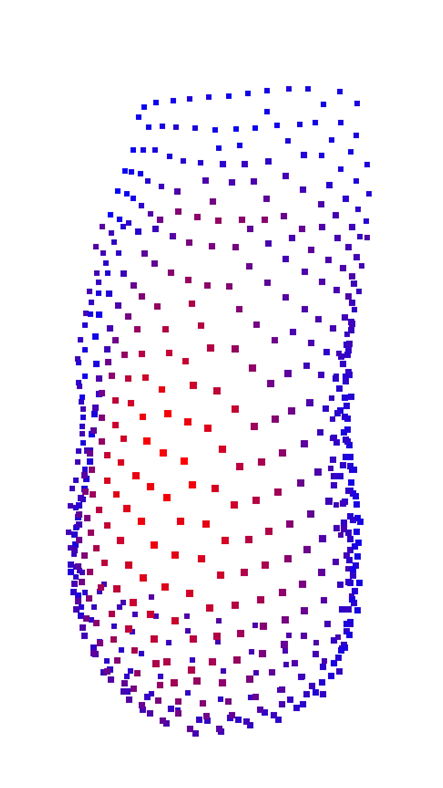
\includegraphics[width = 3.5in]{heatmap_1}} &
\subfloat[]{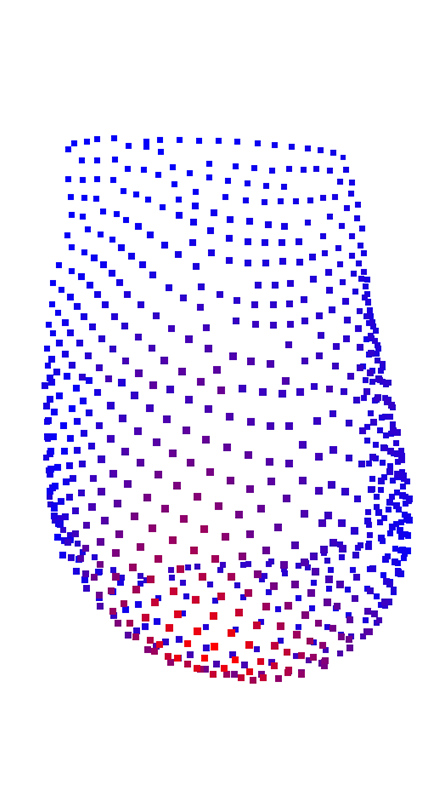
\includegraphics[width = 3.5in]{heatmap_2}}
\end{tabular}
}
\caption[Prediction errors heatmap]{Prediction errors heatmap}
\label{fig:heatmap}
\end{figure}

As expected, the parts of the breast where a greater number of predictive errors exist are coincident with the regions of the breast near to the tumor's location. This regions are more likely to present larger errors, since they are the most affected ones by the deformations caused by the BCS. The points of the breast that are closer to what would be the pectoral muscle, do not present errors.

\section{Summary}

This chapter presented the result of the evaluation metrics defined in chapter \ref{chap:method} for the different methods though to be able to predict the deformations of the breast caused by BCS. From the analysis of the same results, conclusions were able to be drawn and are stated during this chapter.

Regarding the overall results, it is possible to conclude that machine learning techniques led to significantly better results than the methods based on common sense and the feature analysis findings. Despite of the prediction error and the need to minimize them, the results show that the prediction of the breast shape on the proposed environment can be done using machine learning techniques and replace the need to use highly time and computational power consuming alternatives like FEM.  
